\documentclass[twoside]{book}

% Packages required by doxygen
\usepackage{calc}
\usepackage{doxygen}
\usepackage{graphicx}
\usepackage[utf8]{inputenc}
\usepackage{makeidx}
\usepackage{multicol}
\usepackage{multirow}
\usepackage{textcomp}
\usepackage[table]{xcolor}

% Font selection
\usepackage[T1]{fontenc}
\usepackage{mathptmx}
\usepackage[scaled=.90]{helvet}
\usepackage{courier}
\usepackage{amssymb}
\usepackage{sectsty}
\renewcommand{\familydefault}{\sfdefault}
\allsectionsfont{%
  \fontseries{bc}\selectfont%
  \color{darkgray}%
}
\renewcommand{\DoxyLabelFont}{%
  \fontseries{bc}\selectfont%
  \color{darkgray}%
}

% Page & text layout
\usepackage{geometry}
\geometry{%
  a4paper,%
  top=2.5cm,%
  bottom=2.5cm,%
  left=2.5cm,%
  right=2.5cm%
}
\tolerance=750
\hfuzz=15pt
\hbadness=750
\setlength{\emergencystretch}{15pt}
\setlength{\parindent}{0cm}
\setlength{\parskip}{0.2cm}
\makeatletter
\renewcommand{\paragraph}{%
  \@startsection{paragraph}{4}{0ex}{-1.0ex}{1.0ex}{%
    \normalfont\normalsize\bfseries\SS@parafont%
  }%
}
\renewcommand{\subparagraph}{%
  \@startsection{subparagraph}{5}{0ex}{-1.0ex}{1.0ex}{%
    \normalfont\normalsize\bfseries\SS@subparafont%
  }%
}
\makeatother

% Headers & footers
\usepackage{fancyhdr}
\pagestyle{fancyplain}
\fancyhead[LE]{\fancyplain{}{\bfseries\thepage}}
\fancyhead[CE]{\fancyplain{}{}}
\fancyhead[RE]{\fancyplain{}{\bfseries\leftmark}}
\fancyhead[LO]{\fancyplain{}{\bfseries\rightmark}}
\fancyhead[CO]{\fancyplain{}{}}
\fancyhead[RO]{\fancyplain{}{\bfseries\thepage}}
\fancyfoot[LE]{\fancyplain{}{}}
\fancyfoot[CE]{\fancyplain{}{}}
\fancyfoot[RE]{\fancyplain{}{\bfseries\scriptsize Generated on Fri Apr 7 2017 15\-:24\-:37 for R\-O\-S Adhoc Communication Node by Doxygen }}
\fancyfoot[LO]{\fancyplain{}{\bfseries\scriptsize Generated on Fri Apr 7 2017 15\-:24\-:37 for R\-O\-S Adhoc Communication Node by Doxygen }}
\fancyfoot[CO]{\fancyplain{}{}}
\fancyfoot[RO]{\fancyplain{}{}}
\renewcommand{\footrulewidth}{0.4pt}
\renewcommand{\chaptermark}[1]{%
  \markboth{#1}{}%
}
\renewcommand{\sectionmark}[1]{%
  \markright{\thesection\ #1}%
}

% Indices & bibliography
\usepackage{natbib}
\usepackage[titles]{tocloft}
\setcounter{tocdepth}{3}
\setcounter{secnumdepth}{5}
\makeindex

% Hyperlinks (required, but should be loaded last)
\usepackage{ifpdf}
\ifpdf
  \usepackage[pdftex,pagebackref=true]{hyperref}
\else
  \usepackage[ps2pdf,pagebackref=true]{hyperref}
\fi
\hypersetup{%
  colorlinks=true,%
  linkcolor=blue,%
  citecolor=blue,%
  unicode%
}

% Custom commands
\newcommand{\clearemptydoublepage}{%
  \newpage{\pagestyle{empty}\cleardoublepage}%
}


%===== C O N T E N T S =====

\begin{document}

% Titlepage & ToC
\hypersetup{pageanchor=false}
\pagenumbering{roman}
\begin{titlepage}
\vspace*{7cm}
\begin{center}%
{\Large R\-O\-S Adhoc Communication Node }\\
\vspace*{1cm}
{\large Generated by Doxygen 1.8.6}\\
\vspace*{0.5cm}
{\small Fri Apr 7 2017 15:24:37}\\
\end{center}
\end{titlepage}
\clearemptydoublepage
\tableofcontents
\clearemptydoublepage
\pagenumbering{arabic}
\hypersetup{pageanchor=true}

%--- Begin generated contents ---
\chapter{Todo List}
\label{todo}
\hypertarget{todo}{}

\begin{DoxyRefList}
\item[\label{todo__todo000001}%
\hypertarget{todo__todo000001}{}%
Global \hyperlink{classMcRouteActivationFrame_a2a6ad3848eb8318aa6eb332552cc4f9a}{Mc\-Route\-Activation\-Frame\-:\-:Mc\-Route\-Activation\-Frame} (unsigned char $\ast$next\-\_\-hop, std\-::string mc\-\_\-g, uint32\-\_\-t route\-\_\-id, std\-::string source)]Eventually not final const. 
\begin{DoxyParams}{Parameters}
{\em disconnect} & \\
\hline
\end{DoxyParams}
Eventually not final konnst 
\begin{DoxyParams}{Parameters}
{\em disconnect} & \\
\hline
\end{DoxyParams}
Eventually not final konnst  
\item[\label{todo__todo000003}%
\hypertarget{todo__todo000003}{}%
Global \hyperlink{classPacket_a6eee220fed8f687022dde8c2a162080e}{Packet\-:\-:data\-\_\-type\-\_\-} ]What is this?  
\item[\label{todo__todo000004}%
\hypertarget{todo__todo000004}{}%
Global \hyperlink{classPacket_af17876338c2f107655106432b5a6c2fd}{Packet\-:\-:frames\-\_\-l\-\_\-} ]What is this?  
\item[\label{todo__todo000002}%
\hypertarget{todo__todo000002}{}%
Global \hyperlink{classPacket_aeff54aea0863db044a2948d38895e8aa}{Packet\-:\-:get\-Payload} ()]what?, false otherwise. 
\end{DoxyRefList}
\chapter{Hierarchical Index}
\section{Class Hierarchy}
This inheritance list is sorted roughly, but not completely, alphabetically\-:\begin{DoxyCompactList}
\item \contentsline{section}{ack\-\_\-cr\-\_\-info}{\pageref{structack__cr__info}}{}
\item \contentsline{section}{ack\-\_\-lf\-\_\-header}{\pageref{structack__lf__header}}{}
\item \contentsline{section}{ack\-\_\-rf\-\_\-header}{\pageref{structack__rf__header}}{}
\item \contentsline{section}{bcasts}{\pageref{structbcasts}}{}
\item \contentsline{section}{Beacon}{\pageref{classBeacon}}{}
\item \contentsline{section}{cr\-\_\-detec\-\_\-header}{\pageref{structcr__detec__header}}{}
\item \contentsline{section}{cr\-\_\-entry}{\pageref{structcr__entry}}{}
\item \contentsline{section}{cr\-\_\-route}{\pageref{structcr__route}}{}
\item \contentsline{section}{cr\-\_\-selection\-\_\-header}{\pageref{structcr__selection__header}}{}
\item \contentsline{section}{eh\-\_\-header}{\pageref{structeh__header}}{}
\item \contentsline{section}{Ethernet\-Frame}{\pageref{classEthernetFrame}}{}
\begin{DoxyCompactList}
\item \contentsline{section}{Ack\-Link\-Frame}{\pageref{classAckLinkFrame}}{}
\item \contentsline{section}{Ack\-Routed\-Frame}{\pageref{classAckRoutedFrame}}{}
\item \contentsline{section}{Cr\-Detection\-Frame}{\pageref{classCrDetectionFrame}}{}
\item \contentsline{section}{Cr\-Selection\-Frame}{\pageref{classCrSelectionFrame}}{}
\item \contentsline{section}{Mc\-Ack\-Frame}{\pageref{classMcAckFrame}}{}
\item \contentsline{section}{Mc\-Disconnect\-Frame}{\pageref{classMcDisconnectFrame}}{}
\item \contentsline{section}{Mc\-Nack\-Frame}{\pageref{classMcNackFrame}}{}
\item \contentsline{section}{Mc\-Route\-Activation\-Frame}{\pageref{classMcRouteActivationFrame}}{}
\item \contentsline{section}{Multi\-Hop\-Broadcast\-Frame}{\pageref{classMultiHopBroadcastFrame}}{}
\item \contentsline{section}{Routed\-Frame}{\pageref{classRoutedFrame}}{}
\item \contentsline{section}{Route\-Request}{\pageref{classRouteRequest}}{}
\end{DoxyCompactList}
\item \contentsline{section}{hostname\-\_\-mac}{\pageref{structhostname__mac}}{}
\item \contentsline{section}{Logging}{\pageref{classLogging}}{}
\item \contentsline{section}{mac}{\pageref{structmac}}{}
\item \contentsline{section}{mc\-\_\-ack\-\_\-header}{\pageref{structmc__ack__header}}{}
\item \contentsline{section}{mc\-\_\-act\-\_\-header}{\pageref{structmc__act__header}}{}
\item \contentsline{section}{mc\-\_\-disc\-\_\-header}{\pageref{structmc__disc__header}}{}
\item \contentsline{section}{mc\-\_\-nack\-\_\-header}{\pageref{structmc__nack__header}}{}
\item \contentsline{section}{mc\-\_\-tree}{\pageref{structmc__tree}}{}
\item \contentsline{section}{Mc\-Handler}{\pageref{classMcHandler}}{}
\item \contentsline{section}{Mc\-Pos\-Ack\-Obj}{\pageref{classMcPosAckObj}}{}
\item \contentsline{section}{Mc\-Tree}{\pageref{classMcTree}}{}
\item \contentsline{section}{mh\-\_\-bcast\-\_\-header}{\pageref{structmh__bcast__header}}{}
\item \contentsline{section}{Packet}{\pageref{classPacket}}{}
\item \contentsline{section}{Position\-Subscriber}{\pageref{classPositionSubscriber}}{}
\item \contentsline{section}{relay\-\_\-infos}{\pageref{structrelay__infos}}{}
\item \contentsline{section}{rf\-\_\-header}{\pageref{structrf__header}}{}
\item \contentsline{section}{route\-\_\-request}{\pageref{structroute__request}}{}
\item \contentsline{section}{Route\-Response}{\pageref{classRouteResponse}}{}
\item \contentsline{section}{routing\-\_\-entry}{\pageref{structrouting__entry}}{}
\item \contentsline{section}{rreq\-\_\-header}{\pageref{structrreq__header}}{}
\item \contentsline{section}{stc\-\_\-ack}{\pageref{structstc__ack}}{}
\item \contentsline{section}{stc\-\_\-frame}{\pageref{structstc__frame}}{}
\item \contentsline{section}{stc\-\_\-packet}{\pageref{structstc__packet}}{}
\item \contentsline{section}{stc\-\_\-\-Routed\-Frame}{\pageref{structstc__RoutedFrame}}{}
\end{DoxyCompactList}

\chapter{Data Structure Index}
\section{Data Structures}
Here are the data structures with brief descriptions\-:\begin{DoxyCompactList}
\item\contentsline{section}{\hyperlink{structack__cr__info}{ack\-\_\-cr\-\_\-info} }{\pageref{structack__cr__info}}{}
\item\contentsline{section}{\hyperlink{structack__lf__header}{ack\-\_\-lf\-\_\-header} }{\pageref{structack__lf__header}}{}
\item\contentsline{section}{\hyperlink{structack__rf__header}{ack\-\_\-rf\-\_\-header} }{\pageref{structack__rf__header}}{}
\item\contentsline{section}{\hyperlink{classAckLinkFrame}{Ack\-Link\-Frame} }{\pageref{classAckLinkFrame}}{}
\item\contentsline{section}{\hyperlink{classAckRoutedFrame}{Ack\-Routed\-Frame} }{\pageref{classAckRoutedFrame}}{}
\item\contentsline{section}{\hyperlink{structbcasts}{bcasts} }{\pageref{structbcasts}}{}
\item\contentsline{section}{\hyperlink{classBeacon}{Beacon} \\*Beacons are transmitted periodically to enable robot detection }{\pageref{classBeacon}}{}
\item\contentsline{section}{\hyperlink{structcr__detec__header}{cr\-\_\-detec\-\_\-header} }{\pageref{structcr__detec__header}}{}
\item\contentsline{section}{\hyperlink{structcr__entry}{cr\-\_\-entry} }{\pageref{structcr__entry}}{}
\item\contentsline{section}{\hyperlink{structcr__route}{cr\-\_\-route} }{\pageref{structcr__route}}{}
\item\contentsline{section}{\hyperlink{structcr__selection__header}{cr\-\_\-selection\-\_\-header} }{\pageref{structcr__selection__header}}{}
\item\contentsline{section}{\hyperlink{classCrDetectionFrame}{Cr\-Detection\-Frame} }{\pageref{classCrDetectionFrame}}{}
\item\contentsline{section}{\hyperlink{classCrSelectionFrame}{Cr\-Selection\-Frame} }{\pageref{classCrSelectionFrame}}{}
\item\contentsline{section}{\hyperlink{structeh__header}{eh\-\_\-header} }{\pageref{structeh__header}}{}
\item\contentsline{section}{\hyperlink{classEthernetFrame}{Ethernet\-Frame} }{\pageref{classEthernetFrame}}{}
\item\contentsline{section}{\hyperlink{structhostname__mac}{hostname\-\_\-mac} }{\pageref{structhostname__mac}}{}
\item\contentsline{section}{\hyperlink{classLogging}{Logging} }{\pageref{classLogging}}{}
\item\contentsline{section}{\hyperlink{structmac}{mac} }{\pageref{structmac}}{}
\item\contentsline{section}{\hyperlink{structmc__ack__header}{mc\-\_\-ack\-\_\-header} }{\pageref{structmc__ack__header}}{}
\item\contentsline{section}{\hyperlink{structmc__act__header}{mc\-\_\-act\-\_\-header} }{\pageref{structmc__act__header}}{}
\item\contentsline{section}{\hyperlink{structmc__disc__header}{mc\-\_\-disc\-\_\-header} }{\pageref{structmc__disc__header}}{}
\item\contentsline{section}{\hyperlink{structmc__nack__header}{mc\-\_\-nack\-\_\-header} }{\pageref{structmc__nack__header}}{}
\item\contentsline{section}{\hyperlink{structmc__tree}{mc\-\_\-tree} }{\pageref{structmc__tree}}{}
\item\contentsline{section}{\hyperlink{classMcAckFrame}{Mc\-Ack\-Frame} }{\pageref{classMcAckFrame}}{}
\item\contentsline{section}{\hyperlink{classMcDisconnectFrame}{Mc\-Disconnect\-Frame} }{\pageref{classMcDisconnectFrame}}{}
\item\contentsline{section}{\hyperlink{classMcHandler}{Mc\-Handler} }{\pageref{classMcHandler}}{}
\item\contentsline{section}{\hyperlink{classMcNackFrame}{Mc\-Nack\-Frame} }{\pageref{classMcNackFrame}}{}
\item\contentsline{section}{\hyperlink{classMcPosAckObj}{Mc\-Pos\-Ack\-Obj} }{\pageref{classMcPosAckObj}}{}
\item\contentsline{section}{\hyperlink{classMcRouteActivationFrame}{Mc\-Route\-Activation\-Frame} }{\pageref{classMcRouteActivationFrame}}{}
\item\contentsline{section}{\hyperlink{classMcTree}{Mc\-Tree} }{\pageref{classMcTree}}{}
\item\contentsline{section}{\hyperlink{structmh__bcast__header}{mh\-\_\-bcast\-\_\-header} }{\pageref{structmh__bcast__header}}{}
\item\contentsline{section}{\hyperlink{classMultiHopBroadcastFrame}{Multi\-Hop\-Broadcast\-Frame} }{\pageref{classMultiHopBroadcastFrame}}{}
\item\contentsline{section}{\hyperlink{classPacket}{Packet} \\*The packet class for network layer packets }{\pageref{classPacket}}{}
\item\contentsline{section}{\hyperlink{classPositionSubscriber}{Position\-Subscriber} \\*Subscripes to the position of the stage simulation }{\pageref{classPositionSubscriber}}{}
\item\contentsline{section}{\hyperlink{structrelay__infos}{relay\-\_\-infos} }{\pageref{structrelay__infos}}{}
\item\contentsline{section}{\hyperlink{structrf__header}{rf\-\_\-header} }{\pageref{structrf__header}}{}
\item\contentsline{section}{\hyperlink{structroute__request}{route\-\_\-request} }{\pageref{structroute__request}}{}
\item\contentsline{section}{\hyperlink{classRoutedFrame}{Routed\-Frame} \\*The class of a routed frame }{\pageref{classRoutedFrame}}{}
\item\contentsline{section}{\hyperlink{classRouteRequest}{Route\-Request} }{\pageref{classRouteRequest}}{}
\item\contentsline{section}{\hyperlink{classRouteResponse}{Route\-Response} }{\pageref{classRouteResponse}}{}
\item\contentsline{section}{\hyperlink{structrouting__entry}{routing\-\_\-entry} }{\pageref{structrouting__entry}}{}
\item\contentsline{section}{\hyperlink{structrreq__header}{rreq\-\_\-header} }{\pageref{structrreq__header}}{}
\item\contentsline{section}{\hyperlink{structstc__ack}{stc\-\_\-ack} }{\pageref{structstc__ack}}{}
\item\contentsline{section}{\hyperlink{structstc__frame}{stc\-\_\-frame} }{\pageref{structstc__frame}}{}
\item\contentsline{section}{\hyperlink{structstc__packet}{stc\-\_\-packet} }{\pageref{structstc__packet}}{}
\item\contentsline{section}{\hyperlink{structstc__RoutedFrame}{stc\-\_\-\-Routed\-Frame} }{\pageref{structstc__RoutedFrame}}{}
\end{DoxyCompactList}

\chapter{File Index}
\section{File List}
Here is a list of all documented files with brief descriptions\-:\begin{DoxyCompactList}
\item\contentsline{section}{src/{\bfseries Ack\-Link\-Frame.\-h} }{\pageref{AckLinkFrame_8h}}{}
\item\contentsline{section}{src/{\bfseries Ack\-Routed\-Frame.\-h} }{\pageref{AckRoutedFrame_8h}}{}
\item\contentsline{section}{src/{\bfseries Beacon.\-h} }{\pageref{Beacon_8h}}{}
\item\contentsline{section}{src/{\bfseries Cr\-Detection\-Frame.\-h} }{\pageref{CrDetectionFrame_8h}}{}
\item\contentsline{section}{src/{\bfseries Cr\-Selection\-Frame.\-h} }{\pageref{CrSelectionFrame_8h}}{}
\item\contentsline{section}{src/{\bfseries Debug\-Functions.\-h} }{\pageref{DebugFunctions_8h}}{}
\item\contentsline{section}{src/{\bfseries defines.\-h} }{\pageref{defines_8h}}{}
\item\contentsline{section}{src/{\bfseries Ethernet\-Frame.\-h} }{\pageref{EthernetFrame_8h}}{}
\item\contentsline{section}{src/{\bfseries functions.\-h} }{\pageref{functions_8h}}{}
\item\contentsline{section}{src/{\bfseries header.\-h} }{\pageref{header_8h}}{}
\item\contentsline{section}{src/{\bfseries Logging.\-h} }{\pageref{Logging_8h}}{}
\item\contentsline{section}{src/{\bfseries Mc\-Ack\-Frame.\-h} }{\pageref{McAckFrame_8h}}{}
\item\contentsline{section}{src/{\bfseries Mc\-Disconnect\-Frame.\-h} }{\pageref{McDisconnectFrame_8h}}{}
\item\contentsline{section}{src/{\bfseries Mc\-Handler.\-h} }{\pageref{McHandler_8h}}{}
\item\contentsline{section}{src/{\bfseries Mc\-Nack\-Frame.\-h} }{\pageref{McNackFrame_8h}}{}
\item\contentsline{section}{src/{\bfseries Mc\-Pos\-Ack\-Obj.\-h} }{\pageref{McPosAckObj_8h}}{}
\item\contentsline{section}{src/{\bfseries Mc\-Route\-Activation\-Frame.\-h} }{\pageref{McRouteActivationFrame_8h}}{}
\item\contentsline{section}{src/{\bfseries Mc\-Tree.\-h} }{\pageref{McTree_8h}}{}
\item\contentsline{section}{src/{\bfseries Multi\-Hop\-Broadcast\-Frame.\-h} }{\pageref{MultiHopBroadcastFrame_8h}}{}
\item\contentsline{section}{src/\hyperlink{Packet_8h}{Packet.\-h} \\*Network layer packet definition }{\pageref{Packet_8h}}{}
\item\contentsline{section}{src/\hyperlink{PositionSubscriber_8h}{Position\-Subscriber.\-h} }{\pageref{PositionSubscriber_8h}}{}
\item\contentsline{section}{src/\hyperlink{RoutedFrame_8cpp}{Routed\-Frame.\-cpp} \\*Network layer packet definition }{\pageref{RoutedFrame_8cpp}}{}
\item\contentsline{section}{src/{\bfseries Routed\-Frame.\-h} }{\pageref{RoutedFrame_8h}}{}
\item\contentsline{section}{src/{\bfseries Route\-Request.\-h} }{\pageref{RouteRequest_8h}}{}
\item\contentsline{section}{src/{\bfseries Route\-Response.\-h} }{\pageref{RouteResponse_8h}}{}
\item\contentsline{section}{src/{\bfseries structs.\-h} }{\pageref{structs_8h}}{}
\end{DoxyCompactList}

\chapter{Data Structure Documentation}
\hypertarget{structack__cr__info}{\section{ack\-\_\-cr\-\_\-info Struct Reference}
\label{structack__cr__info}\index{ack\-\_\-cr\-\_\-info@{ack\-\_\-cr\-\_\-info}}
}
\subsection*{Public Member Functions}
\begin{DoxyCompactItemize}
\item 
\hypertarget{structack__cr__info_a26bf03e8d05773efdd0b6b011cf5b85b}{bool {\bfseries operator==} (const \hyperlink{structack__cr__info}{ack\-\_\-cr\-\_\-info} \&p)}\label{structack__cr__info_a26bf03e8d05773efdd0b6b011cf5b85b}

\end{DoxyCompactItemize}
\subsection*{Data Fields}
\begin{DoxyCompactItemize}
\item 
\hypertarget{structack__cr__info_ae1adc5a36bc0b0cec0d13e44a2378519}{unsigned char {\bfseries frame\-\_\-src\-\_\-mac} \mbox{[}6\mbox{]}}\label{structack__cr__info_ae1adc5a36bc0b0cec0d13e44a2378519}

\item 
\hypertarget{structack__cr__info_ab1dc8d3ff8da2011155ebc36f155cfec}{unsigned char {\bfseries frame\-\_\-dst\-\_\-mac} \mbox{[}6\mbox{]}}\label{structack__cr__info_ab1dc8d3ff8da2011155ebc36f155cfec}

\item 
\hypertarget{structack__cr__info_ac377b17e56bdbec3ebe5069aa94e2508}{uint32\-\_\-t {\bfseries id}}\label{structack__cr__info_ac377b17e56bdbec3ebe5069aa94e2508}

\item 
\hypertarget{structack__cr__info_ace8975310c3aa06cb660e1f9eeec5a94}{uint32\-\_\-t {\bfseries seq}}\label{structack__cr__info_ace8975310c3aa06cb660e1f9eeec5a94}

\item 
\hypertarget{structack__cr__info_ae305fb09165abd104507c90b74d51b94}{unsigned long {\bfseries ts}}\label{structack__cr__info_ae305fb09165abd104507c90b74d51b94}

\item 
\hypertarget{structack__cr__info_a9775625a36d38934b63cc4312b089c58}{std\-::string {\bfseries source\-\_\-host}}\label{structack__cr__info_a9775625a36d38934b63cc4312b089c58}

\item 
\hypertarget{structack__cr__info_ab585640607fc3311d981fa9c8c0e1e5b}{std\-::string {\bfseries mc\-\_\-group}}\label{structack__cr__info_ab585640607fc3311d981fa9c8c0e1e5b}

\item 
\hypertarget{structack__cr__info_a2c8e0d4be3c0fe42212b21de47e0cbb3}{bool {\bfseries retransmitted}}\label{structack__cr__info_a2c8e0d4be3c0fe42212b21de47e0cbb3}

\item 
\hypertarget{structack__cr__info_a7a664545d7cb43b60528cdd98d920e16}{std\-::string {\bfseries network\-\_\-string}}\label{structack__cr__info_a7a664545d7cb43b60528cdd98d920e16}

\item 
\hypertarget{structack__cr__info_a8369e5f06e6f45c06d74ffc584e025e7}{uint8\-\_\-t {\bfseries frame\-\_\-type}}\label{structack__cr__info_a8369e5f06e6f45c06d74ffc584e025e7}

\end{DoxyCompactItemize}


The documentation for this struct was generated from the following file\-:\begin{DoxyCompactItemize}
\item 
src/structs.\-h\end{DoxyCompactItemize}

\hypertarget{structack__lf__header}{\section{ack\-\_\-lf\-\_\-header Struct Reference}
\label{structack__lf__header}\index{ack\-\_\-lf\-\_\-header@{ack\-\_\-lf\-\_\-header}}
}
\subsection*{Data Fields}
\begin{DoxyCompactItemize}
\item 
\hypertarget{structack__lf__header_aa1bc16939bb29911d15536eda49fb5b1}{uint8\-\_\-t {\bfseries frame\-\_\-type}}\label{structack__lf__header_aa1bc16939bb29911d15536eda49fb5b1}

\item 
\hypertarget{structack__lf__header_ac7d7fdba59d6a4e7c61ca8ea76b7a8f9}{unsigned char {\bfseries mac\-\_\-destination\-\_\-} \mbox{[}6\mbox{]}}\label{structack__lf__header_ac7d7fdba59d6a4e7c61ca8ea76b7a8f9}

\item 
\hypertarget{structack__lf__header_a1dd6d818e8e2c88fcc31d7fc32ea9266}{unsigned char {\bfseries mac\-\_\-confirmer} \mbox{[}6\mbox{]}}\label{structack__lf__header_a1dd6d818e8e2c88fcc31d7fc32ea9266}

\item 
\hypertarget{structack__lf__header_a7838a12d17fddd85d399971d27a85c49}{uint8\-\_\-t {\bfseries ack\-\_\-frame\-\_\-type}}\label{structack__lf__header_a7838a12d17fddd85d399971d27a85c49}

\item 
\hypertarget{structack__lf__header_a71b653ceb8590c8aebd418c10d1a66d1}{uint32\-\_\-t {\bfseries frame\-\_\-id}}\label{structack__lf__header_a71b653ceb8590c8aebd418c10d1a66d1}

\item 
\hypertarget{structack__lf__header_a1a60357ddbb969cadef3efdf53da53a1}{uint8\-\_\-t {\bfseries flag\-\_\-field}}\label{structack__lf__header_a1a60357ddbb969cadef3efdf53da53a1}

\item 
\hypertarget{structack__lf__header_a9360b94aa6d12bb333c3b4b1201d958a}{uint32\-\_\-t {\bfseries hostname\-\_\-source\-\_\-len}}\label{structack__lf__header_a9360b94aa6d12bb333c3b4b1201d958a}

\end{DoxyCompactItemize}


The documentation for this struct was generated from the following file\-:\begin{DoxyCompactItemize}
\item 
src/Ack\-Link\-Frame.\-h\end{DoxyCompactItemize}

\hypertarget{structack__rf__header}{\section{ack\-\_\-rf\-\_\-header Struct Reference}
\label{structack__rf__header}\index{ack\-\_\-rf\-\_\-header@{ack\-\_\-rf\-\_\-header}}
}
\subsection*{Data Fields}
\begin{DoxyCompactItemize}
\item 
\hypertarget{structack__rf__header_a8922f626b1cc2c00818173b6f0ca10e9}{uint8\-\_\-t {\bfseries frame\-\_\-type}}\label{structack__rf__header_a8922f626b1cc2c00818173b6f0ca10e9}

\item 
\hypertarget{structack__rf__header_a4eaa4aaac4f84d10792c817efd5c96f8}{unsigned char {\bfseries mac\-\_\-destination\-\_\-} \mbox{[}6\mbox{]}}\label{structack__rf__header_a4eaa4aaac4f84d10792c817efd5c96f8}

\item 
\hypertarget{structack__rf__header_aee851335668e469b0d9223e3f500f861}{uint32\-\_\-t {\bfseries frame\-\_\-id}}\label{structack__rf__header_aee851335668e469b0d9223e3f500f861}

\item 
\hypertarget{structack__rf__header_a7a8a56154e7656aba02f98170c3195bc}{uint32\-\_\-t {\bfseries route\-\_\-id}}\label{structack__rf__header_a7a8a56154e7656aba02f98170c3195bc}

\item 
\hypertarget{structack__rf__header_ae387a253f9ec8cfc41efae375eee415c}{uint8\-\_\-t {\bfseries flag\-\_\-field}}\label{structack__rf__header_ae387a253f9ec8cfc41efae375eee415c}

\item 
\hypertarget{structack__rf__header_a98d61dbb8d9be735fbc46fc8a90880d2}{uint32\-\_\-t {\bfseries hostname\-\_\-source\-\_\-len}}\label{structack__rf__header_a98d61dbb8d9be735fbc46fc8a90880d2}

\item 
\hypertarget{structack__rf__header_a678665b28262b3fa620e8b6f10d377e3}{uint32\-\_\-t {\bfseries mc\-\_\-group\-\_\-len}}\label{structack__rf__header_a678665b28262b3fa620e8b6f10d377e3}

\end{DoxyCompactItemize}


The documentation for this struct was generated from the following file\-:\begin{DoxyCompactItemize}
\item 
src/Ack\-Routed\-Frame.\-h\end{DoxyCompactItemize}

\hypertarget{classAckLinkFrame}{\section{Ack\-Link\-Frame Class Reference}
\label{classAckLinkFrame}\index{Ack\-Link\-Frame@{Ack\-Link\-Frame}}
}
Inheritance diagram for Ack\-Link\-Frame\-:\begin{figure}[H]
\begin{center}
\leavevmode
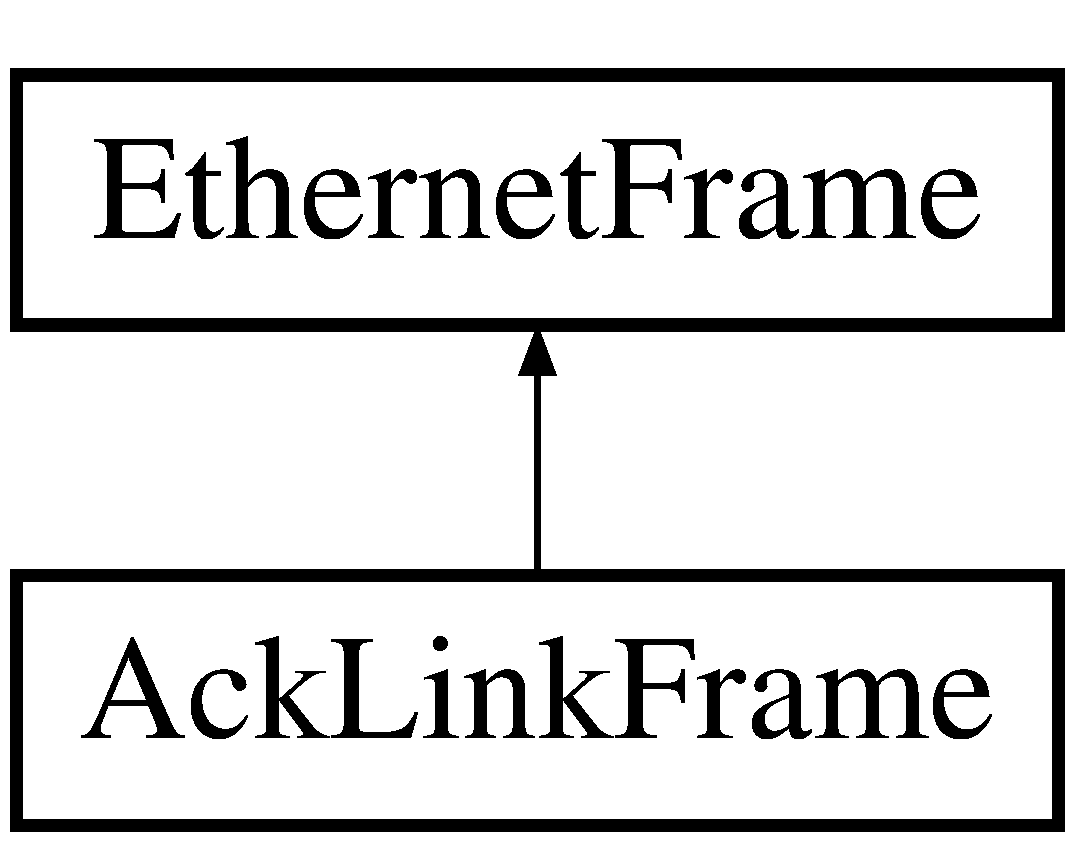
\includegraphics[height=2.000000cm]{classAckLinkFrame}
\end{center}
\end{figure}
\subsection*{Public Member Functions}
\begin{DoxyCompactItemize}
\item 
\hypertarget{classAckLinkFrame_afb4084034a4d610bb3775fafcdb566c6}{{\bfseries Ack\-Link\-Frame} (unsigned char $\ast$source, unsigned char $\ast$confirmer\-\_\-mac, unsigned char $\ast$dest, uint32\-\_\-t frame\-\_\-id, std\-::string hostname, uint8\-\_\-t type)}\label{classAckLinkFrame_afb4084034a4d610bb3775fafcdb566c6}

\item 
\hypertarget{classAckLinkFrame_a83f34f1e35f7bf1ea279055998b504b9}{{\bfseries Ack\-Link\-Frame} (unsigned char $\ast$buffer)}\label{classAckLinkFrame_a83f34f1e35f7bf1ea279055998b504b9}

\item 
\hypertarget{classAckLinkFrame_a42d1b042178c29c366eb9c3787025bd7}{std\-::string {\bfseries get\-Frame\-As\-Network\-String} ()}\label{classAckLinkFrame_a42d1b042178c29c366eb9c3787025bd7}

\item 
\hypertarget{classAckLinkFrame_aa3e501d1e93dcf5c61a3db1480d4afb2}{void {\bfseries print\-\_\-frame} ()}\label{classAckLinkFrame_aa3e501d1e93dcf5c61a3db1480d4afb2}

\end{DoxyCompactItemize}
\subsection*{Data Fields}
\begin{DoxyCompactItemize}
\item 
\hypertarget{classAckLinkFrame_ac860e1f06ef53be350ae1e65ceabe151}{struct \hyperlink{structack__lf__header}{ack\-\_\-lf\-\_\-header} {\bfseries header\-\_\-}}\label{classAckLinkFrame_ac860e1f06ef53be350ae1e65ceabe151}

\item 
\hypertarget{classAckLinkFrame_a88088f732bdeec470a86a4170debcd69}{std\-::string {\bfseries hostname\-\_\-source\-\_\-}}\label{classAckLinkFrame_a88088f732bdeec470a86a4170debcd69}

\item 
\hypertarget{classAckLinkFrame_af572f7dd3f8c75aa32ac5e4a0859d990}{bool {\bfseries pos\-\_\-ack\-\_\-flag\-\_\-}}\label{classAckLinkFrame_af572f7dd3f8c75aa32ac5e4a0859d990}

\item 
\hypertarget{classAckLinkFrame_a65e7d3de4d6eb35d760f70e1a877980b}{bool {\bfseries cr\-\_\-flag\-\_\-}}\label{classAckLinkFrame_a65e7d3de4d6eb35d760f70e1a877980b}

\item 
\hypertarget{classAckLinkFrame_a93e07e53838187874578ed6355d3a795}{uint16\-\_\-t {\bfseries buffer\-\_\-str\-\_\-len\-\_\-}}\label{classAckLinkFrame_a93e07e53838187874578ed6355d3a795}

\end{DoxyCompactItemize}
\subsection*{Static Public Attributes}
\begin{DoxyCompactItemize}
\item 
\hypertarget{classAckLinkFrame_a635114e77539990c03eae1a2cf630c22}{static uint32\-\_\-t {\bfseries H\-E\-A\-D\-E\-R\-\_\-\-F\-I\-X\-E\-D\-\_\-\-L\-E\-N} = sizeof(\hyperlink{structeh__header}{eh\-\_\-header}) + sizeof(\hyperlink{structack__lf__header}{ack\-\_\-lf\-\_\-header})}\label{classAckLinkFrame_a635114e77539990c03eae1a2cf630c22}

\end{DoxyCompactItemize}


The documentation for this class was generated from the following files\-:\begin{DoxyCompactItemize}
\item 
src/Ack\-Link\-Frame.\-h\item 
src/Ack\-Link\-Frame.\-cpp\end{DoxyCompactItemize}

\hypertarget{classAckRoutedFrame}{\section{Ack\-Routed\-Frame Class Reference}
\label{classAckRoutedFrame}\index{Ack\-Routed\-Frame@{Ack\-Routed\-Frame}}
}
Inheritance diagram for Ack\-Routed\-Frame\-:\begin{figure}[H]
\begin{center}
\leavevmode
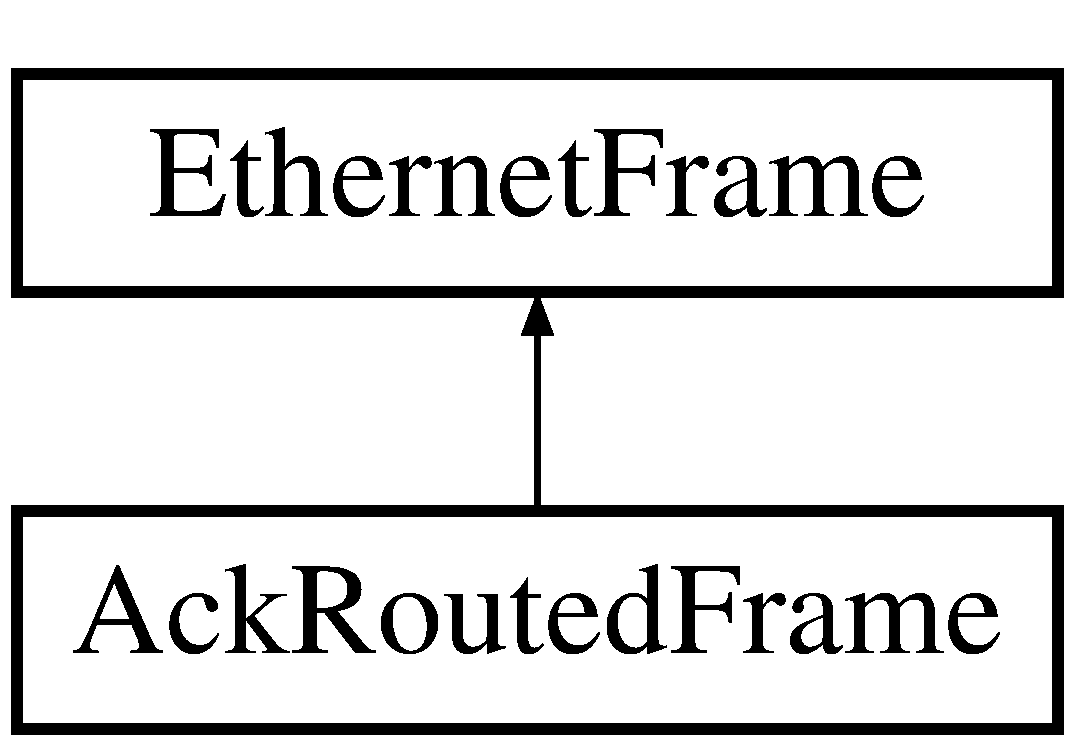
\includegraphics[height=2.000000cm]{classAckRoutedFrame}
\end{center}
\end{figure}
\subsection*{Public Member Functions}
\begin{DoxyCompactItemize}
\item 
\hypertarget{classAckRoutedFrame_ae1a29aa32b72d22f118148dd7bd519a8}{{\bfseries Ack\-Routed\-Frame} (\hyperlink{classRoutedFrame}{Routed\-Frame} rf)}\label{classAckRoutedFrame_ae1a29aa32b72d22f118148dd7bd519a8}

\item 
\hypertarget{classAckRoutedFrame_a4bd70e8a50d8332a8a6e0444950556a0}{{\bfseries Ack\-Routed\-Frame} (unsigned char $\ast$buffer)}\label{classAckRoutedFrame_a4bd70e8a50d8332a8a6e0444950556a0}

\item 
\hypertarget{classAckRoutedFrame_a900e8f5878a7e433e1fcff23408ca156}{\hyperlink{structstc__frame}{stc\-\_\-frame} {\bfseries get\-Frame\-Struct} ()}\label{classAckRoutedFrame_a900e8f5878a7e433e1fcff23408ca156}

\item 
\hypertarget{classAckRoutedFrame_a23f197ccf7ca36f02f0b662d357b8202}{std\-::string {\bfseries get\-Frame\-As\-Network\-String} (uint32\-\_\-t route\-\_\-id, unsigned char next\-\_\-hop\mbox{[}6\mbox{]}, string source\-\_\-host, unsigned char source\mbox{[}6\mbox{]})}\label{classAckRoutedFrame_a23f197ccf7ca36f02f0b662d357b8202}

\item 
\hypertarget{classAckRoutedFrame_a4d22b4cff6ab2697bceca35335a4e4d5}{std\-::string {\bfseries get\-Frame\-As\-Network\-String} (\hyperlink{structrouting__entry}{routing\-\_\-entry} r, unsigned char src\mbox{[}6\mbox{]})}\label{classAckRoutedFrame_a4d22b4cff6ab2697bceca35335a4e4d5}

\end{DoxyCompactItemize}
\subsection*{Data Fields}
\begin{DoxyCompactItemize}
\item 
\hypertarget{classAckRoutedFrame_a8ed6f1c431816752761ca4449c639745}{struct \hyperlink{structack__rf__header}{ack\-\_\-rf\-\_\-header} {\bfseries header\-\_\-}}\label{classAckRoutedFrame_a8ed6f1c431816752761ca4449c639745}

\item 
\hypertarget{classAckRoutedFrame_ac358556a646d660a4e8a8861c368ee3a}{std\-::string {\bfseries hostname\-\_\-source\-\_\-}}\label{classAckRoutedFrame_ac358556a646d660a4e8a8861c368ee3a}

\item 
\hypertarget{classAckRoutedFrame_a58fa10cc3b9c106ab85e0652295ae4e0}{std\-::string {\bfseries mc\-\_\-group\-\_\-}}\label{classAckRoutedFrame_a58fa10cc3b9c106ab85e0652295ae4e0}

\item 
\hypertarget{classAckRoutedFrame_a76ab978d90be8f4594c982fabab5e9c3}{uint32\-\_\-t {\bfseries buffer\-\_\-str\-\_\-len\-\_\-}}\label{classAckRoutedFrame_a76ab978d90be8f4594c982fabab5e9c3}

\item 
\hypertarget{classAckRoutedFrame_a70643e91f2c5d16b1eee0ceef62846fd}{bool {\bfseries cr\-\_\-flag}}\label{classAckRoutedFrame_a70643e91f2c5d16b1eee0ceef62846fd}

\item 
\hypertarget{classAckRoutedFrame_a065ec75f6db7c7d03bb746fbab51bd24}{bool {\bfseries mc\-\_\-flag}}\label{classAckRoutedFrame_a065ec75f6db7c7d03bb746fbab51bd24}

\end{DoxyCompactItemize}
\subsection*{Static Public Attributes}
\begin{DoxyCompactItemize}
\item 
\hypertarget{classAckRoutedFrame_ad00f23365e9f2f0ad8e573e155946f4d}{static uint32\-\_\-t {\bfseries H\-E\-A\-D\-E\-R\-\_\-\-F\-I\-X\-E\-D\-\_\-\-L\-E\-N} = sizeof (\hyperlink{structeh__header}{eh\-\_\-header}) + sizeof (\hyperlink{structack__rf__header}{ack\-\_\-rf\-\_\-header})}\label{classAckRoutedFrame_ad00f23365e9f2f0ad8e573e155946f4d}

\end{DoxyCompactItemize}


The documentation for this class was generated from the following files\-:\begin{DoxyCompactItemize}
\item 
src/Ack\-Routed\-Frame.\-h\item 
src/Ack\-Routed\-Frame.\-cpp\end{DoxyCompactItemize}

\hypertarget{structbcasts}{\section{bcasts Struct Reference}
\label{structbcasts}\index{bcasts@{bcasts}}
}
\subsection*{Public Member Functions}
\begin{DoxyCompactItemize}
\item 
\hypertarget{structbcasts_aef827206ae76754a35d2d373a25ca6be}{{\bfseries bcasts} (uint32\-\_\-t id\-\_\-, std\-::string src\-\_\-)}\label{structbcasts_aef827206ae76754a35d2d373a25ca6be}

\item 
\hypertarget{structbcasts_a94063dfe921d2dee1a9a8f5e63058a57}{bool {\bfseries operator==} (const \hyperlink{structbcasts}{bcasts} \&st)}\label{structbcasts_a94063dfe921d2dee1a9a8f5e63058a57}

\end{DoxyCompactItemize}
\subsection*{Data Fields}
\begin{DoxyCompactItemize}
\item 
\hypertarget{structbcasts_adcc0cb59c6231cf2b56b9d3c33e618e2}{uint32\-\_\-t {\bfseries id}}\label{structbcasts_adcc0cb59c6231cf2b56b9d3c33e618e2}

\item 
\hypertarget{structbcasts_a398832cace36378e74fe269ba7064413}{std\-::string {\bfseries src}}\label{structbcasts_a398832cace36378e74fe269ba7064413}

\end{DoxyCompactItemize}


The documentation for this struct was generated from the following file\-:\begin{DoxyCompactItemize}
\item 
src/structs.\-h\end{DoxyCompactItemize}

\hypertarget{classBeacon}{\section{Beacon Class Reference}
\label{classBeacon}\index{Beacon@{Beacon}}
}


Beacons are transmitted periodically to enable robot detection.  




{\ttfamily \#include $<$Beacon.\-h$>$}

\subsection*{Public Member Functions}
\begin{DoxyCompactItemize}
\item 
\hyperlink{classBeacon_aaffc4541f12325619271033678112f9f}{Beacon} (unsigned char $\ast$source, std\-::string hostname)
\begin{DoxyCompactList}\small\item\em Constructs the \hyperlink{classBeacon}{Beacon} on the sender side. \end{DoxyCompactList}\item 
\hyperlink{classBeacon_a2c2bd4621a255efdf2f60076b00cd683}{Beacon} (unsigned char $\ast$buffer)
\begin{DoxyCompactList}\small\item\em Constructs the \hyperlink{classBeacon}{Beacon} on the receiver side. \end{DoxyCompactList}\item 
std\-::string \hyperlink{classBeacon_acc9536d578591492b2a09064667d09d2}{get\-Frame\-As\-Network\-String} ()
\begin{DoxyCompactList}\small\item\em Returns a \hyperlink{classBeacon}{Beacon} as a C++ string. \end{DoxyCompactList}\item 
int \hyperlink{classBeacon_a85a0dbb4be299c38792b5b6c12f40e8b}{Get\-Crc32} (const std\-::string \&my\-\_\-string)
\begin{DoxyCompactList}\small\item\em Calculates the Crc32 of a \hyperlink{classBeacon}{Beacon} Is needed to detect corrupt beacons caused by transmission errors. \end{DoxyCompactList}\end{DoxyCompactItemize}
\subsection*{Data Fields}
\begin{DoxyCompactItemize}
\item 
\hypertarget{classBeacon_abab167ece2947c117638cde893c425f8}{bool \hyperlink{classBeacon_abab167ece2947c117638cde893c425f8}{correct\-\_\-crc\-\_\-}}\label{classBeacon_abab167ece2947c117638cde893c425f8}

\begin{DoxyCompactList}\small\item\em Indicates whether C\-R\-C of received beacon is correct. \end{DoxyCompactList}\item 
\hypertarget{classBeacon_a72c5f38f3e5b28af976f6d7281969fe9}{unsigned char \hyperlink{classBeacon_a72c5f38f3e5b28af976f6d7281969fe9}{mac\-\_\-source\-\_\-} \mbox{[}6\mbox{]}}\label{classBeacon_a72c5f38f3e5b28af976f6d7281969fe9}

\begin{DoxyCompactList}\small\item\em The mac address of the source robot that emits the \hyperlink{classBeacon}{Beacon}. \end{DoxyCompactList}\item 
\hypertarget{classBeacon_a4655e5fdc179bb569c8b3bf33feca048}{struct ethhdr $\ast$ \hyperlink{classBeacon_a4655e5fdc179bb569c8b3bf33feca048}{eh\-\_\-}}\label{classBeacon_a4655e5fdc179bb569c8b3bf33feca048}

\begin{DoxyCompactList}\small\item\em Defines layer 2 Ethernet header. \end{DoxyCompactList}\item 
\hypertarget{classBeacon_a8cac0cdb11df430d406e1ab55e1dde58}{std\-::string \hyperlink{classBeacon_a8cac0cdb11df430d406e1ab55e1dde58}{hostname\-\_\-}}\label{classBeacon_a8cac0cdb11df430d406e1ab55e1dde58}

\begin{DoxyCompactList}\small\item\em Stores host name of the beacon sender. \end{DoxyCompactList}\end{DoxyCompactItemize}
\subsection*{Static Public Attributes}
\begin{DoxyCompactItemize}
\item 
\hypertarget{classBeacon_ad65dea59cbc7803632b693e41709f409}{static uint32\-\_\-t \hyperlink{classBeacon_ad65dea59cbc7803632b693e41709f409}{H\-E\-A\-D\-E\-R\-\_\-\-F\-I\-X\-E\-D\-\_\-\-L\-E\-N} = 23}\label{classBeacon_ad65dea59cbc7803632b693e41709f409}

\begin{DoxyCompactList}\small\item\em The lenght of the beacon header (23 bytes) \end{DoxyCompactList}\end{DoxyCompactItemize}


\subsection{Detailed Description}
Beacons are transmitted periodically to enable robot detection. 

They allow to
\begin{DoxyItemize}
\item detect new robots and
\item track connectivity between robots. 
\end{DoxyItemize}

\subsection{Constructor \& Destructor Documentation}
\hypertarget{classBeacon_aaffc4541f12325619271033678112f9f}{\index{Beacon@{Beacon}!Beacon@{Beacon}}
\index{Beacon@{Beacon}!Beacon@{Beacon}}
\subsubsection[{Beacon}]{\setlength{\rightskip}{0pt plus 5cm}Beacon\-::\-Beacon (
\begin{DoxyParamCaption}
\item[{unsigned char $\ast$}]{source, }
\item[{std\-::string}]{hostname}
\end{DoxyParamCaption}
)}}\label{classBeacon_aaffc4541f12325619271033678112f9f}


Constructs the \hyperlink{classBeacon}{Beacon} on the sender side. 


\begin{DoxyParams}{Parameters}
{\em source} & The mac address of the source robot that emits the \hyperlink{classBeacon}{Beacon} \\
\hline
{\em hostname} & The hostname of the source robot that emits the \hyperlink{classBeacon}{Beacon} \\
\hline
\end{DoxyParams}
\hypertarget{classBeacon_a2c2bd4621a255efdf2f60076b00cd683}{\index{Beacon@{Beacon}!Beacon@{Beacon}}
\index{Beacon@{Beacon}!Beacon@{Beacon}}
\subsubsection[{Beacon}]{\setlength{\rightskip}{0pt plus 5cm}Beacon\-::\-Beacon (
\begin{DoxyParamCaption}
\item[{unsigned char $\ast$}]{buffer}
\end{DoxyParamCaption}
)}}\label{classBeacon_a2c2bd4621a255efdf2f60076b00cd683}


Constructs the \hyperlink{classBeacon}{Beacon} on the receiver side. 


\begin{DoxyParams}{Parameters}
{\em buffer} & The received network buffer \\
\hline
\end{DoxyParams}


\subsection{Member Function Documentation}
\hypertarget{classBeacon_a85a0dbb4be299c38792b5b6c12f40e8b}{\index{Beacon@{Beacon}!Get\-Crc32@{Get\-Crc32}}
\index{Get\-Crc32@{Get\-Crc32}!Beacon@{Beacon}}
\subsubsection[{Get\-Crc32}]{\setlength{\rightskip}{0pt plus 5cm}int Beacon\-::\-Get\-Crc32 (
\begin{DoxyParamCaption}
\item[{const std\-::string \&}]{my\-\_\-string}
\end{DoxyParamCaption}
)}}\label{classBeacon_a85a0dbb4be299c38792b5b6c12f40e8b}


Calculates the Crc32 of a \hyperlink{classBeacon}{Beacon} Is needed to detect corrupt beacons caused by transmission errors. 

\begin{DoxyReturn}{Returns}
the Crc32 checksum of a \hyperlink{classBeacon}{Beacon}. 
\end{DoxyReturn}
\hypertarget{classBeacon_acc9536d578591492b2a09064667d09d2}{\index{Beacon@{Beacon}!get\-Frame\-As\-Network\-String@{get\-Frame\-As\-Network\-String}}
\index{get\-Frame\-As\-Network\-String@{get\-Frame\-As\-Network\-String}!Beacon@{Beacon}}
\subsubsection[{get\-Frame\-As\-Network\-String}]{\setlength{\rightskip}{0pt plus 5cm}std\-::string Beacon\-::get\-Frame\-As\-Network\-String (
\begin{DoxyParamCaption}
{}
\end{DoxyParamCaption}
)}}\label{classBeacon_acc9536d578591492b2a09064667d09d2}


Returns a \hyperlink{classBeacon}{Beacon} as a C++ string. 

Converts the beacon into a C++ string to be written to the socket. \begin{DoxyReturn}{Returns}
Bacon as C++ string. 
\end{DoxyReturn}


The documentation for this class was generated from the following files\-:\begin{DoxyCompactItemize}
\item 
src/Beacon.\-h\item 
src/Beacon.\-cpp\end{DoxyCompactItemize}

\hypertarget{structcr__detec__header}{\section{cr\-\_\-detec\-\_\-header Struct Reference}
\label{structcr__detec__header}\index{cr\-\_\-detec\-\_\-header@{cr\-\_\-detec\-\_\-header}}
}
\subsection*{Data Fields}
\begin{DoxyCompactItemize}
\item 
\hypertarget{structcr__detec__header_af61fd84e93789bf12d80f2732f187d5e}{uint8\-\_\-t {\bfseries frame\-\_\-type}}\label{structcr__detec__header_af61fd84e93789bf12d80f2732f187d5e}

\item 
\hypertarget{structcr__detec__header_af549d044df1a6a40b5b63ee70b02f8df}{unsigned char {\bfseries mac1} \mbox{[}6\mbox{]}}\label{structcr__detec__header_af549d044df1a6a40b5b63ee70b02f8df}

\item 
\hypertarget{structcr__detec__header_ac8ebecef9205b865066990a037276eff}{unsigned char {\bfseries mac2} \mbox{[}6\mbox{]}}\label{structcr__detec__header_ac8ebecef9205b865066990a037276eff}

\end{DoxyCompactItemize}


The documentation for this struct was generated from the following file\-:\begin{DoxyCompactItemize}
\item 
src/Cr\-Detection\-Frame.\-h\end{DoxyCompactItemize}

\hypertarget{structcr__entry}{\section{cr\-\_\-entry Struct Reference}
\label{structcr__entry}\index{cr\-\_\-entry@{cr\-\_\-entry}}
}
\subsection*{Public Member Functions}
\begin{DoxyCompactItemize}
\item 
\hypertarget{structcr__entry_ab16dc758a9f460c3ce97a3388b8e9e26}{{\bfseries cr\-\_\-entry} (unsigned char $\ast$first\-\_\-m, unsigned char $\ast$second\-\_\-m)}\label{structcr__entry_ab16dc758a9f460c3ce97a3388b8e9e26}

\item 
\hypertarget{structcr__entry_aea8e3782816931c7d4c030bab0116ae8}{void {\bfseries init} ()}\label{structcr__entry_aea8e3782816931c7d4c030bab0116ae8}

\item 
\hypertarget{structcr__entry_a56dce4149a80a30e551b7f3485e3a983}{void {\bfseries print} ()}\label{structcr__entry_a56dce4149a80a30e551b7f3485e3a983}

\item 
\hypertarget{structcr__entry_a440f370c3f8f6e3157de33cf80a56cbf}{uint8\-\_\-t {\bfseries is\-Relay} (unsigned char $\ast$src, unsigned char $\ast$dest)}\label{structcr__entry_a440f370c3f8f6e3157de33cf80a56cbf}

\item 
\hypertarget{structcr__entry_ab749925735267c3b1d3767d10d3d0ca9}{\hyperlink{structcr__route}{cr\-\_\-route} {\bfseries is\-Mc\-Relay} (unsigned char $\ast$src, std\-::string group)}\label{structcr__entry_ab749925735267c3b1d3767d10d3d0ca9}

\item 
\hypertarget{structcr__entry_afb69e7b268b74c6d0a53d8783344a02b}{bool {\bfseries add\-Mc\-Relay\-Connection} (unsigned char $\ast$src, unsigned char $\ast$dest, std\-::string group)}\label{structcr__entry_afb69e7b268b74c6d0a53d8783344a02b}

\item 
\hypertarget{structcr__entry_a5ab654355cbe24fce3e592fcd81a1db9}{bool {\bfseries deactivate} (unsigned char $\ast$\hyperlink{structmac}{mac})}\label{structcr__entry_a5ab654355cbe24fce3e592fcd81a1db9}

\item 
\hypertarget{structcr__entry_ad792c519087718383d17a68bd9bdfe9f}{void {\bfseries activate} (unsigned char $\ast$\hyperlink{structmac}{mac}, uint8\-\_\-t relay\-\_\-index)}\label{structcr__entry_ad792c519087718383d17a68bd9bdfe9f}

\item 
\hypertarget{structcr__entry_a1007ed9a5e41202d25e99fe857075f5c}{bool {\bfseries operator==} (const \hyperlink{structcr__entry}{cr\-\_\-entry} \&p)}\label{structcr__entry_a1007ed9a5e41202d25e99fe857075f5c}

\end{DoxyCompactItemize}
\subsection*{Data Fields}
\begin{DoxyCompactItemize}
\item 
\hypertarget{structcr__entry_a8a5bb126342d63abf27eb962ae3d2cee}{unsigned char {\bfseries first\-\_\-mac} \mbox{[}6\mbox{]}}\label{structcr__entry_a8a5bb126342d63abf27eb962ae3d2cee}

\item 
\hypertarget{structcr__entry_a57e423df02542addb22a741b5deca298}{unsigned char {\bfseries second\-\_\-mac} \mbox{[}6\mbox{]}}\label{structcr__entry_a57e423df02542addb22a741b5deca298}

\item 
\hypertarget{structcr__entry_a038e4b52d4a909a1058668417ef1e8b1}{bool {\bfseries relay\-\_\-4\-\_\-fist\-\_\-mac}}\label{structcr__entry_a038e4b52d4a909a1058668417ef1e8b1}

\item 
\hypertarget{structcr__entry_ab1fe080bfdd486e3ba16b8034f849e6e}{bool {\bfseries relay\-\_\-4\-\_\-second\-\_\-mac}}\label{structcr__entry_ab1fe080bfdd486e3ba16b8034f849e6e}

\item 
\hypertarget{structcr__entry_a7fa35e8f1594178e0a3ff6d52a8c5f26}{bool {\bfseries hop\-\_\-by\-\_\-hop}}\label{structcr__entry_a7fa35e8f1594178e0a3ff6d52a8c5f26}

\item 
\hypertarget{structcr__entry_a8219b274eee48d23ff3cc7d7cea1d8ca}{std\-::vector$<$ std\-::string $>$ {\bfseries group\-\_\-connections\-\_\-first\-\_\-mac}}\label{structcr__entry_a8219b274eee48d23ff3cc7d7cea1d8ca}

\item 
\hypertarget{structcr__entry_a8d6a2a6bb3b0e8bbfe068fbb35fcec3a}{std\-::vector$<$ std\-::string $>$ {\bfseries group\-\_\-connections\-\_\-second\-\_\-mac}}\label{structcr__entry_a8d6a2a6bb3b0e8bbfe068fbb35fcec3a}

\item 
\hypertarget{structcr__entry_a92f4f3e9788073f796c6ddcadf32abae}{uint8\-\_\-t {\bfseries index\-\_\-fist\-\_\-mac}}\label{structcr__entry_a92f4f3e9788073f796c6ddcadf32abae}

\item 
\hypertarget{structcr__entry_a3ed45b5055f761686764255c79fbb174}{uint8\-\_\-t {\bfseries index\-\_\-second\-\_\-mac}}\label{structcr__entry_a3ed45b5055f761686764255c79fbb174}

\item 
\hypertarget{structcr__entry_a6e5025b111b254aa0e6eee4df15f7c40}{list$<$ uint32\-\_\-t $>$ {\bfseries route\-\_\-ids}}\label{structcr__entry_a6e5025b111b254aa0e6eee4df15f7c40}

\end{DoxyCompactItemize}


The documentation for this struct was generated from the following file\-:\begin{DoxyCompactItemize}
\item 
src/structs.\-h\end{DoxyCompactItemize}

\hypertarget{structcr__route}{\section{cr\-\_\-route Struct Reference}
\label{structcr__route}\index{cr\-\_\-route@{cr\-\_\-route}}
}
\subsection*{Data Fields}
\begin{DoxyCompactItemize}
\item 
\hypertarget{structcr__route_a8c107a911b07dc61ddbc161b65f52a6b}{unsigned char {\bfseries src} \mbox{[}6\mbox{]}}\label{structcr__route_a8c107a911b07dc61ddbc161b65f52a6b}

\item 
\hypertarget{structcr__route_a8c561ee495f594e703b7ba593cef90cc}{unsigned char {\bfseries dst} \mbox{[}6\mbox{]}}\label{structcr__route_a8c561ee495f594e703b7ba593cef90cc}

\item 
\hypertarget{structcr__route_a1f4957acaa629d6064af8a2e424aaed6}{uint8\-\_\-t {\bfseries relay\-\_\-index}}\label{structcr__route_a1f4957acaa629d6064af8a2e424aaed6}

\end{DoxyCompactItemize}


The documentation for this struct was generated from the following file\-:\begin{DoxyCompactItemize}
\item 
src/structs.\-h\end{DoxyCompactItemize}

\hypertarget{structcr__selection__header}{\section{cr\-\_\-selection\-\_\-header Struct Reference}
\label{structcr__selection__header}\index{cr\-\_\-selection\-\_\-header@{cr\-\_\-selection\-\_\-header}}
}
\subsection*{Data Fields}
\begin{DoxyCompactItemize}
\item 
\hypertarget{structcr__selection__header_accf13e0ce4578dee3e4fc0e3fd18c4b3}{uint8\-\_\-t {\bfseries frame\-\_\-type}}\label{structcr__selection__header_accf13e0ce4578dee3e4fc0e3fd18c4b3}

\item 
\hypertarget{structcr__selection__header_a2915f582743e48f0fbdbe4e08b404c2e}{uint32\-\_\-t {\bfseries id}}\label{structcr__selection__header_a2915f582743e48f0fbdbe4e08b404c2e}

\item 
\hypertarget{structcr__selection__header_a2ae092e9130f7a35b48a2a32872cc217}{unsigned char {\bfseries relay\-\_\-connection} \mbox{[}6\mbox{]}}\label{structcr__selection__header_a2ae092e9130f7a35b48a2a32872cc217}

\item 
\hypertarget{structcr__selection__header_a314446313c5b64c3b329c725758fe557}{uint8\-\_\-t {\bfseries relay\-\_\-index}}\label{structcr__selection__header_a314446313c5b64c3b329c725758fe557}

\end{DoxyCompactItemize}


The documentation for this struct was generated from the following file\-:\begin{DoxyCompactItemize}
\item 
src/Cr\-Selection\-Frame.\-h\end{DoxyCompactItemize}

\hypertarget{classCrDetectionFrame}{\section{Cr\-Detection\-Frame Class Reference}
\label{classCrDetectionFrame}\index{Cr\-Detection\-Frame@{Cr\-Detection\-Frame}}
}
Inheritance diagram for Cr\-Detection\-Frame\-:\begin{figure}[H]
\begin{center}
\leavevmode
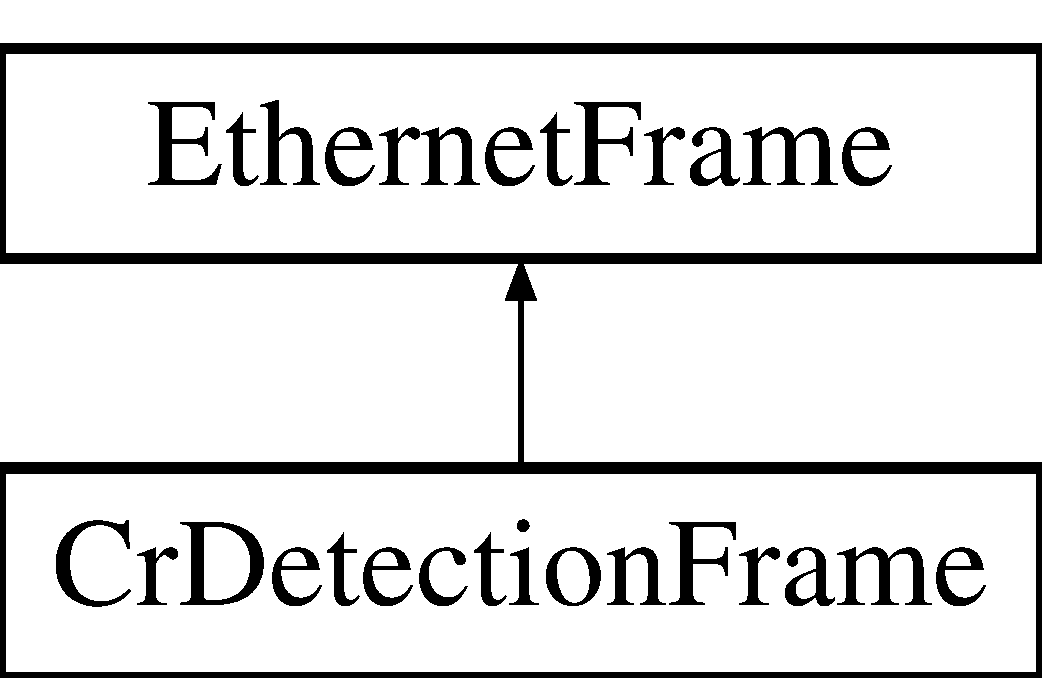
\includegraphics[height=2.000000cm]{classCrDetectionFrame}
\end{center}
\end{figure}
\subsection*{Public Member Functions}
\begin{DoxyCompactItemize}
\item 
\hypertarget{classCrDetectionFrame_ae18f2eb2a6342d0760790cc3bb236cf8}{{\bfseries Cr\-Detection\-Frame} (unsigned char $\ast$first\-\_\-mac, unsigned char $\ast$second\-\_\-mac)}\label{classCrDetectionFrame_ae18f2eb2a6342d0760790cc3bb236cf8}

\item 
\hypertarget{classCrDetectionFrame_a770a7b9e5cf99fc4162e1aa557c15374}{{\bfseries Cr\-Detection\-Frame} (unsigned char $\ast$buffer)}\label{classCrDetectionFrame_a770a7b9e5cf99fc4162e1aa557c15374}

\item 
\hypertarget{classCrDetectionFrame_aa402d5ca474162151698e40d51a08c71}{{\bfseries Cr\-Detection\-Frame} (const \hyperlink{classCrDetectionFrame}{Cr\-Detection\-Frame} \&orig)}\label{classCrDetectionFrame_aa402d5ca474162151698e40d51a08c71}

\item 
\hypertarget{classCrDetectionFrame_ab8b90e0e28d53954ee2ef85ee5d9b173}{std\-::string {\bfseries get\-Frame\-As\-Network\-String} (unsigned char $\ast$src)}\label{classCrDetectionFrame_ab8b90e0e28d53954ee2ef85ee5d9b173}

\end{DoxyCompactItemize}
\subsection*{Data Fields}
\begin{DoxyCompactItemize}
\item 
\hypertarget{classCrDetectionFrame_abef93a118f6acc3026a07a26dfebb66e}{struct \hyperlink{structcr__detec__header}{cr\-\_\-detec\-\_\-header} {\bfseries header\-\_\-}}\label{classCrDetectionFrame_abef93a118f6acc3026a07a26dfebb66e}

\item 
\hypertarget{classCrDetectionFrame_ae1f87912445fb16510d975071a561f0e}{uint32\-\_\-t {\bfseries buffer\-\_\-str\-\_\-len\-\_\-}}\label{classCrDetectionFrame_ae1f87912445fb16510d975071a561f0e}

\end{DoxyCompactItemize}
\subsection*{Static Public Attributes}
\begin{DoxyCompactItemize}
\item 
\hypertarget{classCrDetectionFrame_a5293e3726b046b7a076dc86910e26262}{static uint32\-\_\-t {\bfseries H\-E\-A\-D\-E\-R\-\_\-\-F\-I\-X\-E\-D\-\_\-\-L\-E\-N} = sizeof (\hyperlink{structeh__header}{eh\-\_\-header}) + sizeof (\hyperlink{structcr__detec__header}{cr\-\_\-detec\-\_\-header})}\label{classCrDetectionFrame_a5293e3726b046b7a076dc86910e26262}

\end{DoxyCompactItemize}


The documentation for this class was generated from the following files\-:\begin{DoxyCompactItemize}
\item 
src/Cr\-Detection\-Frame.\-h\item 
src/Cr\-Detection\-Frame.\-cpp\end{DoxyCompactItemize}

\hypertarget{classCrSelectionFrame}{\section{Cr\-Selection\-Frame Class Reference}
\label{classCrSelectionFrame}\index{Cr\-Selection\-Frame@{Cr\-Selection\-Frame}}
}
Inheritance diagram for Cr\-Selection\-Frame\-:\begin{figure}[H]
\begin{center}
\leavevmode
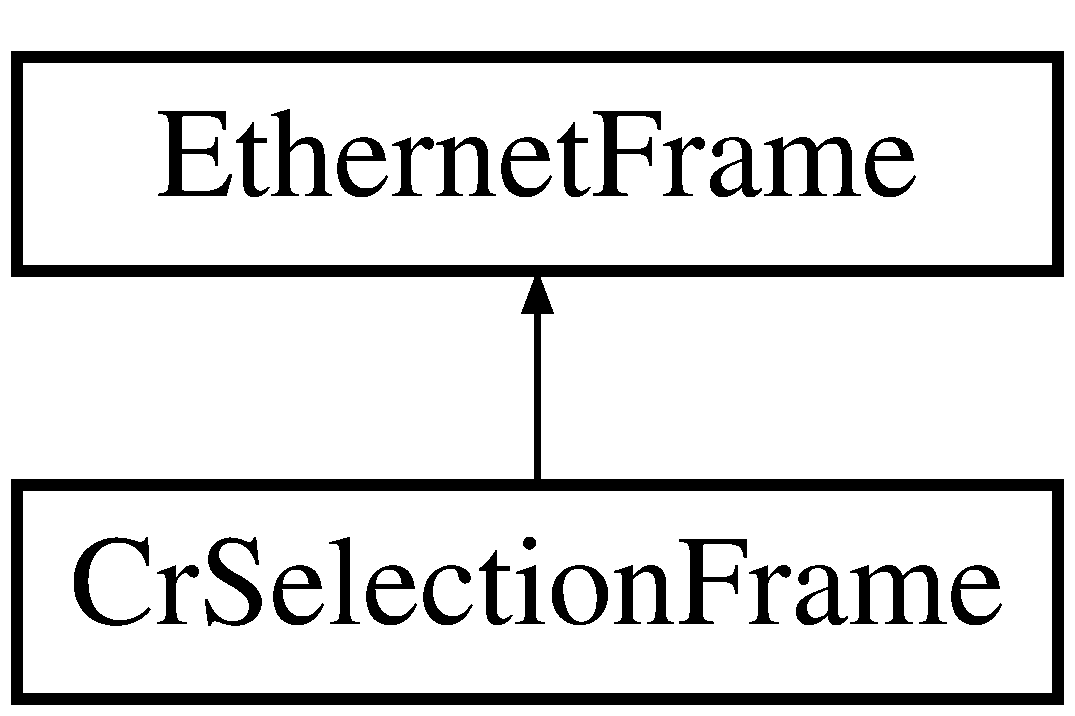
\includegraphics[height=2.000000cm]{classCrSelectionFrame}
\end{center}
\end{figure}
\subsection*{Public Member Functions}
\begin{DoxyCompactItemize}
\item 
\hypertarget{classCrSelectionFrame_a7962f610821bc4dfa979c71f763d4124}{{\bfseries Cr\-Selection\-Frame} (unsigned char $\ast$dst, unsigned char $\ast$relay\-\_\-conn, uint8\-\_\-t relay\-\_\-index)}\label{classCrSelectionFrame_a7962f610821bc4dfa979c71f763d4124}

\item 
\hypertarget{classCrSelectionFrame_a5d4f2f16027449976d8f5ccbc5238fff}{{\bfseries Cr\-Selection\-Frame} (unsigned char $\ast$buffer)}\label{classCrSelectionFrame_a5d4f2f16027449976d8f5ccbc5238fff}

\item 
\hypertarget{classCrSelectionFrame_ad70153db877a687540971e5d793e06fb}{{\bfseries Cr\-Selection\-Frame} (const \hyperlink{classCrSelectionFrame}{Cr\-Selection\-Frame} \&orig)}\label{classCrSelectionFrame_ad70153db877a687540971e5d793e06fb}

\item 
\hypertarget{classCrSelectionFrame_a12ed3b4a1d11e164f90d45586e8da971}{std\-::string {\bfseries get\-Frame\-As\-Network\-String} (unsigned char $\ast$src)}\label{classCrSelectionFrame_a12ed3b4a1d11e164f90d45586e8da971}

\end{DoxyCompactItemize}
\subsection*{Data Fields}
\begin{DoxyCompactItemize}
\item 
\hypertarget{classCrSelectionFrame_aaae48e7f6fe89c5c03e25c3ce8517155}{struct \hyperlink{structcr__selection__header}{cr\-\_\-selection\-\_\-header} {\bfseries header\-\_\-}}\label{classCrSelectionFrame_aaae48e7f6fe89c5c03e25c3ce8517155}

\item 
\hypertarget{classCrSelectionFrame_acc31b7bae9adc7b382e0536f98307a3a}{uint32\-\_\-t {\bfseries buffer\-\_\-str\-\_\-len\-\_\-}}\label{classCrSelectionFrame_acc31b7bae9adc7b382e0536f98307a3a}

\end{DoxyCompactItemize}
\subsection*{Static Public Attributes}
\begin{DoxyCompactItemize}
\item 
\hypertarget{classCrSelectionFrame_a0170c58a2257e86ba0f9a5ca99437ef2}{static uint32\-\_\-t {\bfseries H\-E\-A\-D\-E\-R\-\_\-\-F\-I\-X\-E\-D\-\_\-\-L\-E\-N} = sizeof (\hyperlink{structeh__header}{eh\-\_\-header}) + sizeof (\hyperlink{structcr__selection__header}{cr\-\_\-selection\-\_\-header})}\label{classCrSelectionFrame_a0170c58a2257e86ba0f9a5ca99437ef2}

\item 
\hypertarget{classCrSelectionFrame_a9d6268b45fecf79c51404ae4d367c0f3}{static uint32\-\_\-t {\bfseries frame\-\_\-count\-\_\-stat} = 0}\label{classCrSelectionFrame_a9d6268b45fecf79c51404ae4d367c0f3}

\end{DoxyCompactItemize}


The documentation for this class was generated from the following files\-:\begin{DoxyCompactItemize}
\item 
src/Cr\-Selection\-Frame.\-h\item 
src/Cr\-Selection\-Frame.\-cpp\end{DoxyCompactItemize}

\hypertarget{structeh__header}{\section{eh\-\_\-header Struct Reference}
\label{structeh__header}\index{eh\-\_\-header@{eh\-\_\-header}}
}
\subsection*{Data Fields}
\begin{DoxyCompactItemize}
\item 
\hypertarget{structeh__header_af33cdb71413c6dbe2dbea747f7958e30}{unsigned char {\bfseries eh\-\_\-dest} \mbox{[}6\mbox{]}}\label{structeh__header_af33cdb71413c6dbe2dbea747f7958e30}

\item 
\hypertarget{structeh__header_a38a48a02116d55f38959fc3128eaa999}{unsigned char {\bfseries eh\-\_\-source} \mbox{[}6\mbox{]}}\label{structeh__header_a38a48a02116d55f38959fc3128eaa999}

\item 
\hypertarget{structeh__header_a3056f889bfffa7fdb3ae73afddfdbbf9}{uint16\-\_\-t {\bfseries eh\-\_\-protocol\-\_\-id}}\label{structeh__header_a3056f889bfffa7fdb3ae73afddfdbbf9}

\end{DoxyCompactItemize}


The documentation for this struct was generated from the following file\-:\begin{DoxyCompactItemize}
\item 
src/Ethernet\-Frame.\-h\end{DoxyCompactItemize}

\hypertarget{classEthernetFrame}{\section{Ethernet\-Frame Class Reference}
\label{classEthernetFrame}\index{Ethernet\-Frame@{Ethernet\-Frame}}
}
Inheritance diagram for Ethernet\-Frame\-:\begin{figure}[H]
\begin{center}
\leavevmode
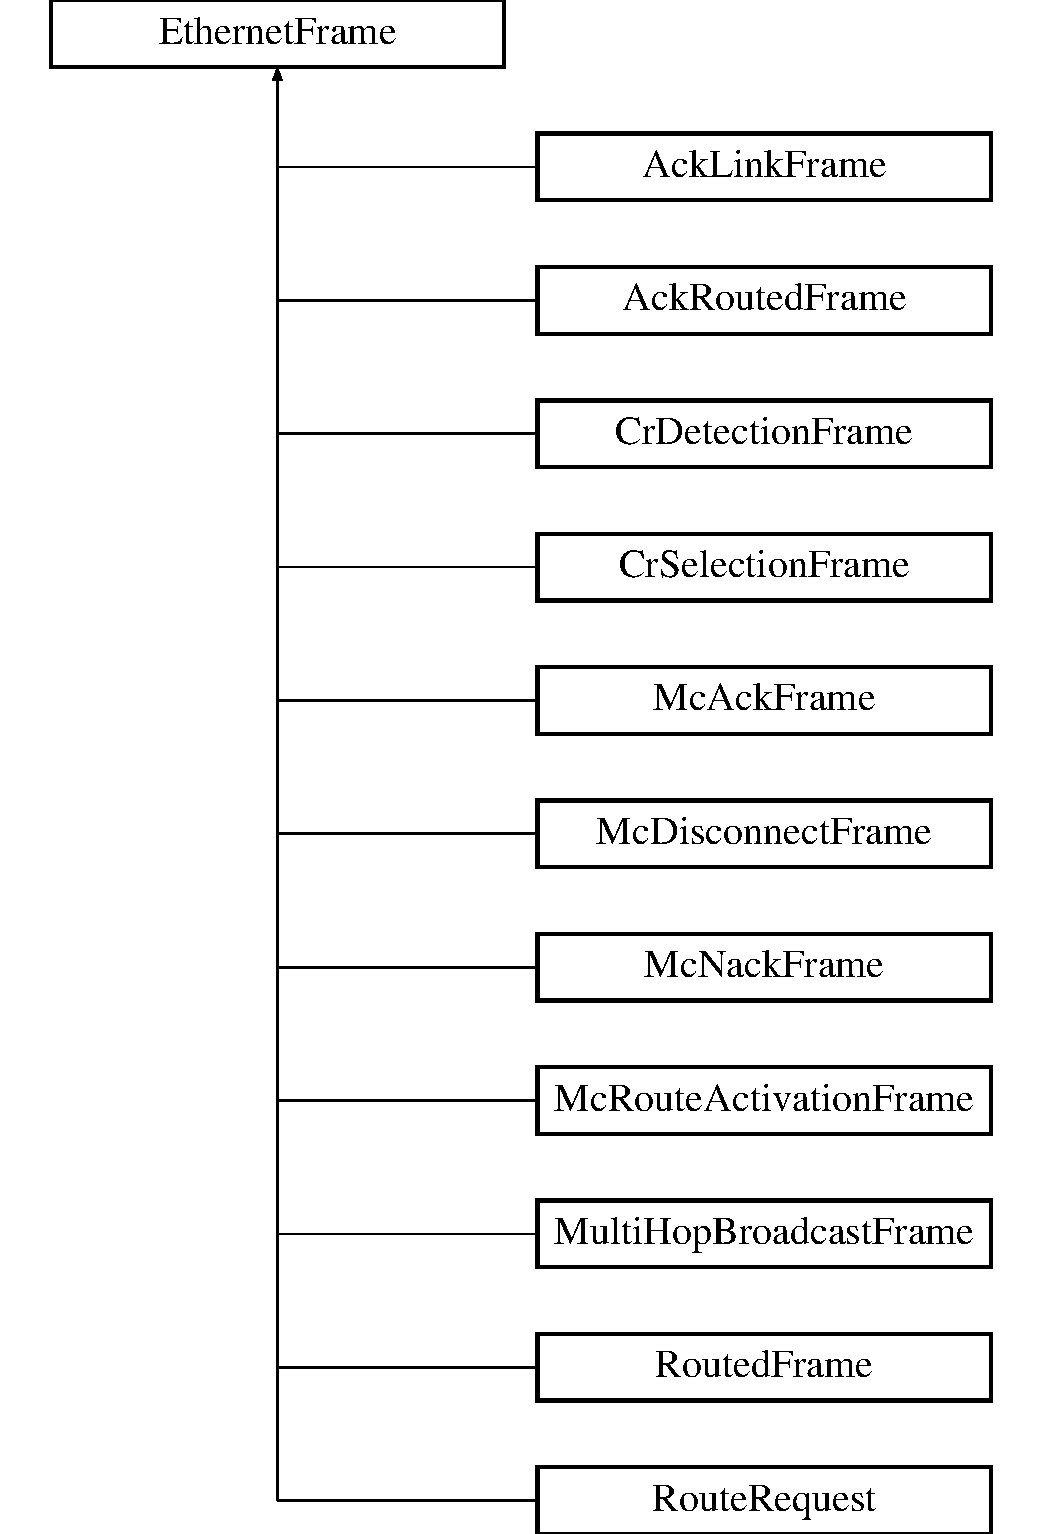
\includegraphics[height=12.000000cm]{classEthernetFrame}
\end{center}
\end{figure}
\subsection*{Public Member Functions}
\begin{DoxyCompactItemize}
\item 
int \hyperlink{classEthernetFrame_a2645ddba8bd1082d6386d77b124da9d3}{Get\-Crc32} (const std\-::string \&string)
\begin{DoxyCompactList}\small\item\em Calculates the Crc32 of the Mc\-Maintenance\-Frame Is needed to detect corrupt frames caused by transmission errors. \end{DoxyCompactList}\end{DoxyCompactItemize}
\subsection*{Data Fields}
\begin{DoxyCompactItemize}
\item 
\hypertarget{classEthernetFrame_a04714f785da3194515926cf43625c0f5}{struct \hyperlink{structeh__header}{eh\-\_\-header} \hyperlink{classEthernetFrame_a04714f785da3194515926cf43625c0f5}{eh\-\_\-h\-\_\-}}\label{classEthernetFrame_a04714f785da3194515926cf43625c0f5}

\begin{DoxyCompactList}\small\item\em Struct of the layer 2 Ethernet header. Includes\-: source mac, destination mac an protocol type. \end{DoxyCompactList}\item 
\hypertarget{classEthernetFrame_a80d45f84327aba98dc33618c5774e345}{bool {\bfseries correct\-\_\-crc\-\_\-}}\label{classEthernetFrame_a80d45f84327aba98dc33618c5774e345}

\end{DoxyCompactItemize}


\subsection{Member Function Documentation}
\hypertarget{classEthernetFrame_a2645ddba8bd1082d6386d77b124da9d3}{\index{Ethernet\-Frame@{Ethernet\-Frame}!Get\-Crc32@{Get\-Crc32}}
\index{Get\-Crc32@{Get\-Crc32}!EthernetFrame@{Ethernet\-Frame}}
\subsubsection[{Get\-Crc32}]{\setlength{\rightskip}{0pt plus 5cm}int Ethernet\-Frame\-::\-Get\-Crc32 (
\begin{DoxyParamCaption}
\item[{const std\-::string \&}]{string}
\end{DoxyParamCaption}
)}}\label{classEthernetFrame_a2645ddba8bd1082d6386d77b124da9d3}


Calculates the Crc32 of the Mc\-Maintenance\-Frame Is needed to detect corrupt frames caused by transmission errors. 

\begin{DoxyReturn}{Returns}
the Crc32 checksum of a Mc\-Maintenance\-Frame. 
\end{DoxyReturn}


The documentation for this class was generated from the following files\-:\begin{DoxyCompactItemize}
\item 
src/Ethernet\-Frame.\-h\item 
src/Ethernet\-Frame.\-cpp\end{DoxyCompactItemize}

\hypertarget{structhostname__mac}{\section{hostname\-\_\-mac Struct Reference}
\label{structhostname__mac}\index{hostname\-\_\-mac@{hostname\-\_\-mac}}
}
\subsection*{Public Member Functions}
\begin{DoxyCompactItemize}
\item 
\hypertarget{structhostname__mac_ac84142944e5ac704e488946ca00cc71c}{{\bfseries hostname\-\_\-mac} (unsigned char $\ast$m)}\label{structhostname__mac_ac84142944e5ac704e488946ca00cc71c}

\item 
\hypertarget{structhostname__mac_a2e519ca449d73a53eb05b8261c4888df}{void {\bfseries stamp} ()}\label{structhostname__mac_a2e519ca449d73a53eb05b8261c4888df}

\item 
\hypertarget{structhostname__mac_a3502a0d7e1a90729f3841e292548c11b}{bool {\bfseries operator==} (const \hyperlink{structhostname__mac}{hostname\-\_\-mac} \&st)}\label{structhostname__mac_a3502a0d7e1a90729f3841e292548c11b}

\end{DoxyCompactItemize}
\subsection*{Data Fields}
\begin{DoxyCompactItemize}
\item 
\hypertarget{structhostname__mac_ac550a99d7eac1467f9e16f8b0e8df6bd}{std\-::string {\bfseries hostname}}\label{structhostname__mac_ac550a99d7eac1467f9e16f8b0e8df6bd}

\item 
\hypertarget{structhostname__mac_a8b5cebe755b3f82251ef197f7805aae3}{unsigned char {\bfseries mac} \mbox{[}6\mbox{]}}\label{structhostname__mac_a8b5cebe755b3f82251ef197f7805aae3}

\item 
\hypertarget{structhostname__mac_a12e6eac4d7e2d23df9f222a68a361915}{bool {\bfseries reachable}}\label{structhostname__mac_a12e6eac4d7e2d23df9f222a68a361915}

\item 
\hypertarget{structhostname__mac_ad0ecf7f66f93ecd39232e47742a82f32}{unsigned long {\bfseries ts}}\label{structhostname__mac_ad0ecf7f66f93ecd39232e47742a82f32}

\end{DoxyCompactItemize}


The documentation for this struct was generated from the following file\-:\begin{DoxyCompactItemize}
\item 
src/structs.\-h\end{DoxyCompactItemize}

\hypertarget{classLogging}{\section{Logging Class Reference}
\label{classLogging}\index{Logging@{Logging}}
}
\subsection*{Public Member Functions}
\begin{DoxyCompactItemize}
\item 
\hypertarget{classLogging_ac6a1c9ea7776cd74f47bde71e38364da}{{\bfseries Logging} (const \hyperlink{classLogging}{Logging} \&orig)}\label{classLogging_ac6a1c9ea7776cd74f47bde71e38364da}

\end{DoxyCompactItemize}
\subsection*{Static Public Member Functions}
\begin{DoxyCompactItemize}
\item 
\hypertarget{classLogging_ac9b0791fcd34355046bf1efcd8933745}{static void {\bfseries init} (ros\-::\-Node\-Handle $\ast$n, std\-::string $\ast$robot\-\_\-name)}\label{classLogging_ac9b0791fcd34355046bf1efcd8933745}

\item 
\hypertarget{classLogging_a6cf79a044b7916c6178d007f0d594fe0}{static void {\bfseries log} ()}\label{classLogging_a6cf79a044b7916c6178d007f0d594fe0}

\item 
\hypertarget{classLogging_a4cd2926447add5daf884531662eb993d}{static bool {\bfseries create\-Log\-Path} ()}\label{classLogging_a4cd2926447add5daf884531662eb993d}

\item 
\hypertarget{classLogging_a982c4a6bc3fc23aa3176658091398005}{static void {\bfseries periodic\-Log} (unsigned long interval\-\_\-ms)}\label{classLogging_a982c4a6bc3fc23aa3176658091398005}

\item 
\hypertarget{classLogging_aa38b526582aadc2bcbaa902ff649fe65}{static void {\bfseries log\-Service\-Calls} (string service\-\_\-name, unsigned long time\-\_\-call, unsigned long time\-\_\-res, unsigned long size, bool ret\-\_\-val)}\label{classLogging_aa38b526582aadc2bcbaa902ff649fe65}

\item 
\hypertarget{classLogging_a5e47b73b1b05a77250cfcd04343d5aa3}{static void {\bfseries log\-Uc\-Packets\-Summary} (unsigned long interval\-\_\-ms)}\label{classLogging_a5e47b73b1b05a77250cfcd04343d5aa3}

\item 
\hypertarget{classLogging_a2280c78af5eed664108d355b7c640a0f}{static void {\bfseries log\-Mc\-Packets\-Summary} (unsigned long interval\-\_\-ms)}\label{classLogging_a2280c78af5eed664108d355b7c640a0f}

\item 
\hypertarget{classLogging_ad9f61b6c59f4b254d57fbdc5224c0637}{static void {\bfseries log\-Memory\-Consumption\-Packets} (unsigned long interval\-\_\-ms, boost\-::mutex $\ast$mtx\-\_\-pack, list$<$ \hyperlink{classPacket}{Packet} $>$ $\ast$packets, boost\-::mutex $\ast$mtx\-\_\-cached\-\_\-mc, list$<$ \hyperlink{classPacket}{Packet} $>$ $\ast$cached\-\_\-mc, boost\-::mutex $\ast$mtx\-\_\-unack\-\_\-link\-\_\-frames, list$<$ \hyperlink{structstc__frame}{stc\-\_\-frame} $>$ $\ast$unack\-\_\-link\-\_\-frames, boost\-::mutex $\ast$mtx\-\_\-unack\-\_\-cr\-\_\-frames, list$<$ \hyperlink{structack__cr__info}{ack\-\_\-cr\-\_\-info} $>$ $\ast$unack\-\_\-cr\-\_\-frames)}\label{classLogging_ad9f61b6c59f4b254d57fbdc5224c0637}

\item 
\hypertarget{classLogging_a2a254e6ee56fdb1fc1f623a566690035}{static void {\bfseries log\-Routing\-Table} (std\-::list$<$ \hyperlink{structrouting__entry}{routing\-\_\-entry} $>$ $\ast$u\-\_\-entries, std\-::list$<$ \hyperlink{classMcTree}{Mc\-Tree} $\ast$ $>$ $\ast$m\-\_\-entries)}\label{classLogging_a2a254e6ee56fdb1fc1f623a566690035}

\item 
\hypertarget{classLogging_a91a975cd0f43e6931c90a48527483ca6}{static void {\bfseries log\-R\-Request\-Initiater} (\hyperlink{structroute__request}{route\-\_\-request} $\ast$req, \hyperlink{structrouting__entry}{routing\-\_\-entry} $\ast$route)}\label{classLogging_a91a975cd0f43e6931c90a48527483ca6}

\item 
\hypertarget{classLogging_a16ccd4cfea65e904d18778a26dae461d}{static void {\bfseries log\-R\-Request\-Intermediate} (\hyperlink{classRouteRequest}{Route\-Request} $\ast$r)}\label{classLogging_a16ccd4cfea65e904d18778a26dae461d}

\item 
\hypertarget{classLogging_ab454eb0a6873f20d9546d965e0581708}{static void {\bfseries log\-Transport\-Frame} (\hyperlink{structstc__RoutedFrame}{stc\-\_\-\-Routed\-Frame} $\ast$f, \hyperlink{structrouting__entry}{routing\-\_\-entry} $\ast$route, unsigned long start\-\_\-time, unsigned long end\-\_\-time, bool success)}\label{classLogging_ab454eb0a6873f20d9546d965e0581708}

\item 
\hypertarget{classLogging_a7eae9741c39ce916e7f9126b2e4bc097}{static void {\bfseries log\-Uc\-Link\-Transmission} (\hyperlink{structstc__frame}{stc\-\_\-frame} f)}\label{classLogging_a7eae9741c39ce916e7f9126b2e4bc097}

\item 
\hypertarget{classLogging_a906bcd09785f88836339d1c00a6544e5}{static void {\bfseries log\-R\-Request\-Receiver} (std\-::string h\-\_\-src, uint32\-\_\-t id, uint16\-\_\-t counter, uint16\-\_\-t hobs, bool selected, std\-::list$<$ \hyperlink{structmac}{mac} $>$ path\-\_\-l)}\label{classLogging_a906bcd09785f88836339d1c00a6544e5}

\item 
\hypertarget{classLogging_afe135237f47a6264a6cb1ec2648e88d5}{static void {\bfseries create\-Log\-File} (std\-::list$<$ std\-::string $>$ $\ast$table, std\-::string $\ast$filename)}\label{classLogging_afe135237f47a6264a6cb1ec2648e88d5}

\item 
\hypertarget{classLogging_a5644203460a5f5098c2b4bb80bb381ee}{static void {\bfseries safe\-Logs} ()}\label{classLogging_a5644203460a5f5098c2b4bb80bb381ee}

\item 
\hypertarget{classLogging_a123636cea9ed17bdc7afa8796c22a12e}{static uint32\-\_\-t {\bfseries get\-Property} (std\-::string prog\-\_\-name)}\label{classLogging_a123636cea9ed17bdc7afa8796c22a12e}

\item 
\hypertarget{classLogging_a42d34adb4b6a22bc96db3504860bde82}{static void {\bfseries increase\-Property} (std\-::string prop\-\_\-name)}\label{classLogging_a42d34adb4b6a22bc96db3504860bde82}

\item 
\hypertarget{classLogging_ae07d9f8a14eed291f5dfbc75b3f01e0d}{static void {\bfseries increase\-Property} (std\-::string prop\-\_\-name, uint32\-\_\-t value)}\label{classLogging_ae07d9f8a14eed291f5dfbc75b3f01e0d}

\item 
\hypertarget{classLogging_a2c225575cf2bd749524562ac8973aba6}{static void {\bfseries decrease\-Property} (std\-::string prop\-\_\-name)}\label{classLogging_a2c225575cf2bd749524562ac8973aba6}

\item 
\hypertarget{classLogging_a40554f45040eebb3c97cd559edee083b}{static void {\bfseries decrease\-Property} (std\-::string prop\-\_\-name, uint32\-\_\-t value)}\label{classLogging_a40554f45040eebb3c97cd559edee083b}

\end{DoxyCompactItemize}
\subsection*{Static Public Attributes}
\begin{DoxyCompactItemize}
\item 
\hypertarget{classLogging_a0bfdf0d48abb9389aa6eae29a83809a5}{static ros\-::\-Node\-Handle $\ast$ {\bfseries n} = N\-U\-L\-L}\label{classLogging_a0bfdf0d48abb9389aa6eae29a83809a5}

\item 
\hypertarget{classLogging_af3628482ac74ada97e157ce34fe2e75a}{static boost\-::mutex {\bfseries mtx\-\_\-logging}}\label{classLogging_af3628482ac74ada97e157ce34fe2e75a}

\item 
\hypertarget{classLogging_a14b5371406a5fbbfe9771b7055c1e38c}{static std\-::map$<$ std\-::string, \\*
uint32\-\_\-t $>$ {\bfseries uint32\-\_\-properties}}\label{classLogging_a14b5371406a5fbbfe9771b7055c1e38c}

\item 
\hypertarget{classLogging_a08c5e75e1e6d41fdaccb26d48b550d87}{static std\-::list$<$ std\-::string $>$ {\bfseries entries\-\_\-r\-\_\-table}}\label{classLogging_a08c5e75e1e6d41fdaccb26d48b550d87}

\item 
\hypertarget{classLogging_aa9bf2ef5f8c6a472a0f43bf7532ea51d}{static std\-::list$<$ std\-::string $>$ {\bfseries entries\-\_\-rreq\-\_\-initi}}\label{classLogging_aa9bf2ef5f8c6a472a0f43bf7532ea51d}

\item 
\hypertarget{classLogging_a97a2b46a48e9962da3da94f125eb3d31}{static std\-::list$<$ std\-::string $>$ {\bfseries entries\-\_\-rreq\-\_\-recv}}\label{classLogging_a97a2b46a48e9962da3da94f125eb3d31}

\item 
\hypertarget{classLogging_abb7414f8928b7e1986d52483c3f524e7}{static std\-::list$<$ std\-::string $>$ {\bfseries entries\-\_\-rreq\-\_\-interm}}\label{classLogging_abb7414f8928b7e1986d52483c3f524e7}

\item 
\hypertarget{classLogging_a3c1cc54cfe7e86ea55d2f037b7222ec7}{static std\-::list$<$ std\-::string $>$ {\bfseries entries\-\_\-mem\-\_\-consumption}}\label{classLogging_a3c1cc54cfe7e86ea55d2f037b7222ec7}

\item 
\hypertarget{classLogging_a6fc3cddf75a735143f8786137e3c1ec0}{static std\-::list$<$ std\-::string $>$ {\bfseries entries\-\_\-uc\-\_\-frames}}\label{classLogging_a6fc3cddf75a735143f8786137e3c1ec0}

\item 
\hypertarget{classLogging_a40b33b75be59b07e8bb9ab5d9684e651}{static std\-::list$<$ std\-::string $>$ {\bfseries entries\-\_\-mc\-\_\-frames}}\label{classLogging_a40b33b75be59b07e8bb9ab5d9684e651}

\item 
\hypertarget{classLogging_a65e150a78c87bdc0622da8f8647cc9ab}{static std\-::list$<$ std\-::string $>$ {\bfseries entries\-\_\-link\-\_\-frames}}\label{classLogging_a65e150a78c87bdc0622da8f8647cc9ab}

\item 
\hypertarget{classLogging_a5e73ca17e77b2468a49ab2743ee075fa}{static std\-::list$<$ std\-::string $>$ {\bfseries entries\-\_\-service\-\_\-calls}}\label{classLogging_a5e73ca17e77b2468a49ab2743ee075fa}

\item 
\hypertarget{classLogging_ad13e4a661cfc7c92273b42a1123e085e}{static std\-::list$<$ std\-::string $>$ {\bfseries entries\-\_\-transport\-\_\-frames}}\label{classLogging_ad13e4a661cfc7c92273b42a1123e085e}

\item 
\hypertarget{classLogging_a95e03e58a66ef793c8adc5a065648ecc}{static std\-::string {\bfseries log\-\_\-path} = \char`\"{}\char`\"{}}\label{classLogging_a95e03e58a66ef793c8adc5a065648ecc}

\item 
\hypertarget{classLogging_a69425aca393177dc880ea61fe6d24462}{static std\-::string {\bfseries routing\-\_\-table\-\_\-file} = \char`\"{}routing\-\_\-table.\-csv\char`\"{}}\label{classLogging_a69425aca393177dc880ea61fe6d24462}

\item 
\hypertarget{classLogging_a51adcb07ad55cafc50765770190f6acf}{static std\-::string {\bfseries route\-\_\-req\-\_\-src\-\_\-file} = \char`\"{}rreq\-\_\-initiater.\-csv\char`\"{}}\label{classLogging_a51adcb07ad55cafc50765770190f6acf}

\item 
\hypertarget{classLogging_a438f2fecc7a2e8433b2c13b7a08f8dd8}{static std\-::string {\bfseries route\-\_\-req\-\_\-dst\-\_\-file} = \char`\"{}rreq\-\_\-receiver.\-csv\char`\"{}}\label{classLogging_a438f2fecc7a2e8433b2c13b7a08f8dd8}

\item 
\hypertarget{classLogging_a5939f060848fa2e67570b9d7591be9df}{static std\-::string {\bfseries route\-\_\-req\-\_\-iterm\-\_\-file} = \char`\"{}rreq\-\_\-intermediate.\-csv\char`\"{}}\label{classLogging_a5939f060848fa2e67570b9d7591be9df}

\item 
\hypertarget{classLogging_a3619464994ccecfd225ecf1c0ff5a9fb}{static std\-::string {\bfseries mem\-\_\-consumption\-\_\-file} = \char`\"{}packet\-\_\-memory\-\_\-consumption.\-csv\char`\"{}}\label{classLogging_a3619464994ccecfd225ecf1c0ff5a9fb}

\item 
\hypertarget{classLogging_acbc1f83a16e0c7d4975f8b2549ede345}{static std\-::string {\bfseries uc\-\_\-frames\-\_\-file} = \char`\"{}unicast\-\_\-datalink\-\_\-transmission\-\_\-summary.\-csv\char`\"{}}\label{classLogging_acbc1f83a16e0c7d4975f8b2549ede345}

\item 
\hypertarget{classLogging_a6cef4ce1d28d43807658dfacfe55d4ca}{static std\-::string {\bfseries mc\-\_\-frames\-\_\-file} = \char`\"{}multicast.\-csv\char`\"{}}\label{classLogging_a6cef4ce1d28d43807658dfacfe55d4ca}

\item 
\hypertarget{classLogging_a4334f9d5202f158c38d83ecf7e0fef65}{static std\-::string {\bfseries link\-\_\-frames\-\_\-file} = \char`\"{}unicast\-\_\-link\-\_\-transmission.\-csv\char`\"{}}\label{classLogging_a4334f9d5202f158c38d83ecf7e0fef65}

\item 
\hypertarget{classLogging_a8c8a57b58cab81a3ed01273a972561c2}{static std\-::string {\bfseries sercice\-\_\-calls\-\_\-file} = \char`\"{}services.\-csv\char`\"{}}\label{classLogging_a8c8a57b58cab81a3ed01273a972561c2}

\item 
\hypertarget{classLogging_aa304f9fb8b6090b74c6af85e57d16a9b}{static std\-::string {\bfseries transport\-\_\-frames\-\_\-file} = \char`\"{}transport\-\_\-frames.\-csv\char`\"{}}\label{classLogging_aa304f9fb8b6090b74c6af85e57d16a9b}

\item 
\hypertarget{classLogging_abb6d88651d3fe9725d8a54a2a8637c2c}{static std\-::string $\ast$ {\bfseries robot\-\_\-name} = N\-U\-L\-L}\label{classLogging_abb6d88651d3fe9725d8a54a2a8637c2c}

\end{DoxyCompactItemize}


The documentation for this class was generated from the following files\-:\begin{DoxyCompactItemize}
\item 
src/Logging.\-h\item 
src/Logging.\-cpp\end{DoxyCompactItemize}

\hypertarget{structmac}{\section{mac Struct Reference}
\label{structmac}\index{mac@{mac}}
}
\subsection*{Public Member Functions}
\begin{DoxyCompactItemize}
\item 
\hypertarget{structmac_ab543436d0c27ddc7d57d1bb20b0fb117}{{\bfseries mac} (unsigned char $\ast$m)}\label{structmac_ab543436d0c27ddc7d57d1bb20b0fb117}

\end{DoxyCompactItemize}
\subsection*{Data Fields}
\begin{DoxyCompactItemize}
\item 
\hypertarget{structmac_a3dee6a8160024aad03e1e57e4538793f}{unsigned char {\bfseries mac\-\_\-adr} \mbox{[}6\mbox{]}}\label{structmac_a3dee6a8160024aad03e1e57e4538793f}

\end{DoxyCompactItemize}


The documentation for this struct was generated from the following file\-:\begin{DoxyCompactItemize}
\item 
src/functions.\-h\end{DoxyCompactItemize}

\hypertarget{structmc__ack__header}{\section{mc\-\_\-ack\-\_\-header Struct Reference}
\label{structmc__ack__header}\index{mc\-\_\-ack\-\_\-header@{mc\-\_\-ack\-\_\-header}}
}
\subsection*{Data Fields}
\begin{DoxyCompactItemize}
\item 
\hypertarget{structmc__ack__header_ac9cb4165753b5440b1712f9282edee25}{uint8\-\_\-t {\bfseries frame\-\_\-type}}\label{structmc__ack__header_ac9cb4165753b5440b1712f9282edee25}

\item 
\hypertarget{structmc__ack__header_a602240a3c7ddbf7d5d9e8b149f5cdd94}{unsigned char {\bfseries mac\-\_\-destination\-\_\-} \mbox{[}6\mbox{]}}\label{structmc__ack__header_a602240a3c7ddbf7d5d9e8b149f5cdd94}

\item 
\hypertarget{structmc__ack__header_a50cdece6a4a8af7874d80c05ac900fbf}{uint32\-\_\-t {\bfseries packet\-\_\-id}}\label{structmc__ack__header_a50cdece6a4a8af7874d80c05ac900fbf}

\item 
\hypertarget{structmc__ack__header_a2770f6a06ebd8a1e0857253d8ceac1a0}{uint32\-\_\-t {\bfseries frame\-\_\-seq\-\_\-num}}\label{structmc__ack__header_a2770f6a06ebd8a1e0857253d8ceac1a0}

\item 
\hypertarget{structmc__ack__header_abb39fe93c37d60de2adbae586ab9a3b0}{uint8\-\_\-t {\bfseries flag\-\_\-field}}\label{structmc__ack__header_abb39fe93c37d60de2adbae586ab9a3b0}

\item 
\hypertarget{structmc__ack__header_a56a55f895a24fe8c4f1d95782fc9cf47}{uint32\-\_\-t {\bfseries hostname\-\_\-source\-\_\-len}}\label{structmc__ack__header_a56a55f895a24fe8c4f1d95782fc9cf47}

\item 
\hypertarget{structmc__ack__header_aa4e25c215cbc5411df2958926d4086a7}{uint32\-\_\-t {\bfseries mc\-\_\-group\-\_\-len}}\label{structmc__ack__header_aa4e25c215cbc5411df2958926d4086a7}

\end{DoxyCompactItemize}


The documentation for this struct was generated from the following file\-:\begin{DoxyCompactItemize}
\item 
src/Mc\-Ack\-Frame.\-h\end{DoxyCompactItemize}

\hypertarget{structmc__act__header}{\section{mc\-\_\-act\-\_\-header Struct Reference}
\label{structmc__act__header}\index{mc\-\_\-act\-\_\-header@{mc\-\_\-act\-\_\-header}}
}
\subsection*{Data Fields}
\begin{DoxyCompactItemize}
\item 
\hypertarget{structmc__act__header_af88db7b3a5158b83f9ad547718dab6c0}{uint8\-\_\-t {\bfseries frame\-\_\-type}}\label{structmc__act__header_af88db7b3a5158b83f9ad547718dab6c0}

\item 
\hypertarget{structmc__act__header_aeef564ece98583af0ed36bd2f74582fd}{uint32\-\_\-t {\bfseries id}}\label{structmc__act__header_aeef564ece98583af0ed36bd2f74582fd}

\item 
\hypertarget{structmc__act__header_a49dcff159fe4cf35585f1ea12dd5d7ab}{uint32\-\_\-t {\bfseries route\-\_\-id}}\label{structmc__act__header_a49dcff159fe4cf35585f1ea12dd5d7ab}

\item 
\hypertarget{structmc__act__header_a88d04f9681b52e76ac7f6dc4e43f27cf}{unsigned char {\bfseries mac\-\_\-destination} \mbox{[}6\mbox{]}}\label{structmc__act__header_a88d04f9681b52e76ac7f6dc4e43f27cf}

\item 
\hypertarget{structmc__act__header_aa8384884b3fd6e4f79530f1bb7c3198f}{uint32\-\_\-t {\bfseries mc\-\_\-group\-\_\-name\-\_\-len}}\label{structmc__act__header_aa8384884b3fd6e4f79530f1bb7c3198f}

\item 
\hypertarget{structmc__act__header_a38439c7a8f0dc8c6f2940bde0bbabd9a}{uint32\-\_\-t {\bfseries hostname\-\_\-source\-\_\-len}}\label{structmc__act__header_a38439c7a8f0dc8c6f2940bde0bbabd9a}

\end{DoxyCompactItemize}


The documentation for this struct was generated from the following file\-:\begin{DoxyCompactItemize}
\item 
src/Mc\-Route\-Activation\-Frame.\-h\end{DoxyCompactItemize}

\hypertarget{structmc__disc__header}{\section{mc\-\_\-disc\-\_\-header Struct Reference}
\label{structmc__disc__header}\index{mc\-\_\-disc\-\_\-header@{mc\-\_\-disc\-\_\-header}}
}
\subsection*{Data Fields}
\begin{DoxyCompactItemize}
\item 
\hypertarget{structmc__disc__header_a0ef358469b62abe2b0224778d692c4a6}{uint8\-\_\-t {\bfseries frame\-\_\-type}}\label{structmc__disc__header_a0ef358469b62abe2b0224778d692c4a6}

\item 
\hypertarget{structmc__disc__header_aebcd55126136a48ea1ad329d1beccc17}{uint32\-\_\-t {\bfseries id}}\label{structmc__disc__header_aebcd55126136a48ea1ad329d1beccc17}

\item 
\hypertarget{structmc__disc__header_a94072ef4f1664f0c6c0dbdc99f6288a4}{unsigned char {\bfseries mac\-\_\-destination} \mbox{[}6\mbox{]}}\label{structmc__disc__header_a94072ef4f1664f0c6c0dbdc99f6288a4}

\item 
\hypertarget{structmc__disc__header_aa9865df12462c89eeb866d8e7642ffbe}{uint8\-\_\-t {\bfseries flag\-\_\-field}}\label{structmc__disc__header_aa9865df12462c89eeb866d8e7642ffbe}

\item 
\hypertarget{structmc__disc__header_aa4edc269c25a3a0fa2a8b0d53fbe5db6}{uint32\-\_\-t {\bfseries mc\-\_\-group\-\_\-name\-\_\-len}}\label{structmc__disc__header_aa4edc269c25a3a0fa2a8b0d53fbe5db6}

\end{DoxyCompactItemize}


The documentation for this struct was generated from the following file\-:\begin{DoxyCompactItemize}
\item 
src/Mc\-Disconnect\-Frame.\-h\end{DoxyCompactItemize}

\hypertarget{structmc__nack__header}{\section{mc\-\_\-nack\-\_\-header Struct Reference}
\label{structmc__nack__header}\index{mc\-\_\-nack\-\_\-header@{mc\-\_\-nack\-\_\-header}}
}
\subsection*{Data Fields}
\begin{DoxyCompactItemize}
\item 
\hypertarget{structmc__nack__header_ad736cea9bec12e7e3f6155aa72d0d410}{uint8\-\_\-t {\bfseries frame\-\_\-type}}\label{structmc__nack__header_ad736cea9bec12e7e3f6155aa72d0d410}

\item 
\hypertarget{structmc__nack__header_afed629fd0a315244f5803976cb78c6d6}{uint32\-\_\-t {\bfseries id}}\label{structmc__nack__header_afed629fd0a315244f5803976cb78c6d6}

\item 
\hypertarget{structmc__nack__header_add97b1d324d455ce9f980e3ffbf6ddbb}{uint32\-\_\-t {\bfseries packet\-\_\-id}}\label{structmc__nack__header_add97b1d324d455ce9f980e3ffbf6ddbb}

\item 
\hypertarget{structmc__nack__header_ab18b33d8b6bc41eb7863f39b7a407ef5}{uint16\-\_\-t {\bfseries frame\-\_\-seq\-\_\-num\-\_\-size}}\label{structmc__nack__header_ab18b33d8b6bc41eb7863f39b7a407ef5}

\item 
\hypertarget{structmc__nack__header_a2e896998f66d2ccc7191625a478e4c38}{uint32\-\_\-t {\bfseries hostname\-\_\-source\-\_\-len}}\label{structmc__nack__header_a2e896998f66d2ccc7191625a478e4c38}

\item 
\hypertarget{structmc__nack__header_a45e48b0def7e75520e8445f4984de79d}{uint32\-\_\-t {\bfseries mc\-\_\-group\-\_\-len}}\label{structmc__nack__header_a45e48b0def7e75520e8445f4984de79d}

\end{DoxyCompactItemize}


The documentation for this struct was generated from the following file\-:\begin{DoxyCompactItemize}
\item 
src/Mc\-Nack\-Frame.\-h\end{DoxyCompactItemize}

\hypertarget{structmc__tree}{\section{mc\-\_\-tree Struct Reference}
\label{structmc__tree}\index{mc\-\_\-tree@{mc\-\_\-tree}}
}
\subsection*{Public Member Functions}
\begin{DoxyCompactItemize}
\item 
\hypertarget{structmc__tree_a770847df89bb178f0c068c42ba9ccb92}{bool {\bfseries operator==} (const \hyperlink{structmc__tree}{mc\-\_\-tree} \&st)}\label{structmc__tree_a770847df89bb178f0c068c42ba9ccb92}

\end{DoxyCompactItemize}
\subsection*{Data Fields}
\begin{DoxyCompactItemize}
\item 
\hypertarget{structmc__tree_af8f1850c28b6de2912e78a96d4028a3f}{std\-::string {\bfseries group\-\_\-name}}\label{structmc__tree_af8f1850c28b6de2912e78a96d4028a3f}

\item 
\hypertarget{structmc__tree_a7492c75e3dcbf5fc3966770d681c79d8}{\hyperlink{structrouting__entry}{routing\-\_\-entry} {\bfseries route\-\_\-uplink}}\label{structmc__tree_a7492c75e3dcbf5fc3966770d681c79d8}

\item 
\hypertarget{structmc__tree_a84ebf022ad007b068e44cefe60954cbd}{std\-::list$<$ \hyperlink{structmac}{mac} $>$ {\bfseries mc\-\_\-downlinks}}\label{structmc__tree_a84ebf022ad007b068e44cefe60954cbd}

\item 
\hypertarget{structmc__tree_a749cfd1c4a02ae6c821e00e9d6f0d05f}{bool {\bfseries member}}\label{structmc__tree_a749cfd1c4a02ae6c821e00e9d6f0d05f}

\item 
\hypertarget{structmc__tree_a3755bba9d747bd106e687a17a2d9be62}{bool {\bfseries active}}\label{structmc__tree_a3755bba9d747bd106e687a17a2d9be62}

\item 
\hypertarget{structmc__tree_a9e19bc882182642a28a4c6c3a57d4726}{bool {\bfseries connected}}\label{structmc__tree_a9e19bc882182642a28a4c6c3a57d4726}

\item 
\hypertarget{structmc__tree_a605297a30634288a5944e4e11db9639c}{bool {\bfseries root}}\label{structmc__tree_a605297a30634288a5944e4e11db9639c}

\item 
\hypertarget{structmc__tree_ae373ff88ceba71b480fe58cdb4b2fbf2}{uint8\-\_\-t {\bfseries root\-\_\-distance}}\label{structmc__tree_ae373ff88ceba71b480fe58cdb4b2fbf2}

\end{DoxyCompactItemize}


The documentation for this struct was generated from the following file\-:\begin{DoxyCompactItemize}
\item 
src/structs.\-h\end{DoxyCompactItemize}

\hypertarget{classMcAckFrame}{\section{Mc\-Ack\-Frame Class Reference}
\label{classMcAckFrame}\index{Mc\-Ack\-Frame@{Mc\-Ack\-Frame}}
}
Inheritance diagram for Mc\-Ack\-Frame\-:\begin{figure}[H]
\begin{center}
\leavevmode
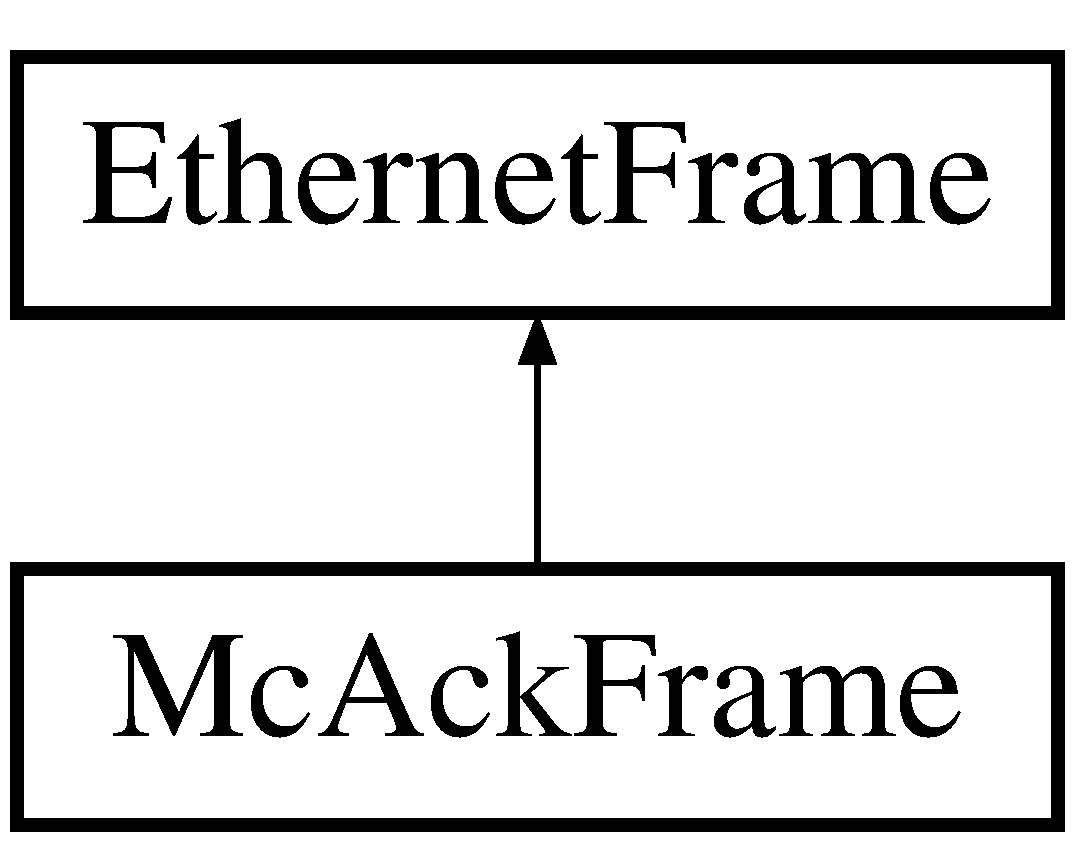
\includegraphics[height=2.000000cm]{classMcAckFrame}
\end{center}
\end{figure}
\subsection*{Public Member Functions}
\begin{DoxyCompactItemize}
\item 
\hypertarget{classMcAckFrame_a6e70d4033528f132e5fa7c08b7b49135}{{\bfseries Mc\-Ack\-Frame} (unsigned char $\ast$source, unsigned char $\ast$dest, std\-::string hostname\-\_\-src, std\-::string group\-\_\-n, uint32\-\_\-t p\-\_\-id, uint32\-\_\-t seq\-\_\-n)}\label{classMcAckFrame_a6e70d4033528f132e5fa7c08b7b49135}

\item 
\hypertarget{classMcAckFrame_abff33c23c0d5856bce2a58ddb00adfec}{{\bfseries Mc\-Ack\-Frame} (unsigned char $\ast$buffer)}\label{classMcAckFrame_abff33c23c0d5856bce2a58ddb00adfec}

\item 
\hypertarget{classMcAckFrame_afb5e987edd755ee472f719b92b71f3e1}{std\-::string {\bfseries get\-Frame\-As\-Network\-String} ()}\label{classMcAckFrame_afb5e987edd755ee472f719b92b71f3e1}

\item 
\hypertarget{classMcAckFrame_a4fc78bb69f8e45e06da316915c74cf76}{void {\bfseries print\-\_\-frame} ()}\label{classMcAckFrame_a4fc78bb69f8e45e06da316915c74cf76}

\end{DoxyCompactItemize}
\subsection*{Data Fields}
\begin{DoxyCompactItemize}
\item 
\hypertarget{classMcAckFrame_a387a487258edc82e4107e4ffa9081029}{struct \hyperlink{structmc__ack__header}{mc\-\_\-ack\-\_\-header} {\bfseries header\-\_\-}}\label{classMcAckFrame_a387a487258edc82e4107e4ffa9081029}

\item 
\hypertarget{classMcAckFrame_ac243aece3e45e022c3c3d2dd2978a7fb}{std\-::string {\bfseries hostname\-\_\-source\-\_\-}}\label{classMcAckFrame_ac243aece3e45e022c3c3d2dd2978a7fb}

\item 
\hypertarget{classMcAckFrame_a008d351c128ff700d8bfab5abaef8020}{std\-::string {\bfseries mc\-\_\-group\-\_\-}}\label{classMcAckFrame_a008d351c128ff700d8bfab5abaef8020}

\item 
\hypertarget{classMcAckFrame_aa7de0709e7c4c89b156bc6def18d9f41}{bool {\bfseries cr\-\_\-flag\-\_\-}}\label{classMcAckFrame_aa7de0709e7c4c89b156bc6def18d9f41}

\item 
\hypertarget{classMcAckFrame_aaa7104cc9db2135e984d8320079e53a2}{uint16\-\_\-t {\bfseries buffer\-\_\-str\-\_\-len\-\_\-}}\label{classMcAckFrame_aaa7104cc9db2135e984d8320079e53a2}

\end{DoxyCompactItemize}
\subsection*{Static Public Attributes}
\begin{DoxyCompactItemize}
\item 
\hypertarget{classMcAckFrame_a060c62e4e65dd045187cac7324f6fb58}{static uint32\-\_\-t {\bfseries H\-E\-A\-D\-E\-R\-\_\-\-F\-I\-X\-E\-D\-\_\-\-L\-E\-N} = sizeof (\hyperlink{structeh__header}{eh\-\_\-header}) + sizeof (\hyperlink{structmc__ack__header}{mc\-\_\-ack\-\_\-header})}\label{classMcAckFrame_a060c62e4e65dd045187cac7324f6fb58}

\end{DoxyCompactItemize}


The documentation for this class was generated from the following files\-:\begin{DoxyCompactItemize}
\item 
src/Mc\-Ack\-Frame.\-h\item 
src/Mc\-Ack\-Frame.\-cpp\end{DoxyCompactItemize}

\hypertarget{classMcDisconnectFrame}{\section{Mc\-Disconnect\-Frame Class Reference}
\label{classMcDisconnectFrame}\index{Mc\-Disconnect\-Frame@{Mc\-Disconnect\-Frame}}
}
Inheritance diagram for Mc\-Disconnect\-Frame\-:\begin{figure}[H]
\begin{center}
\leavevmode
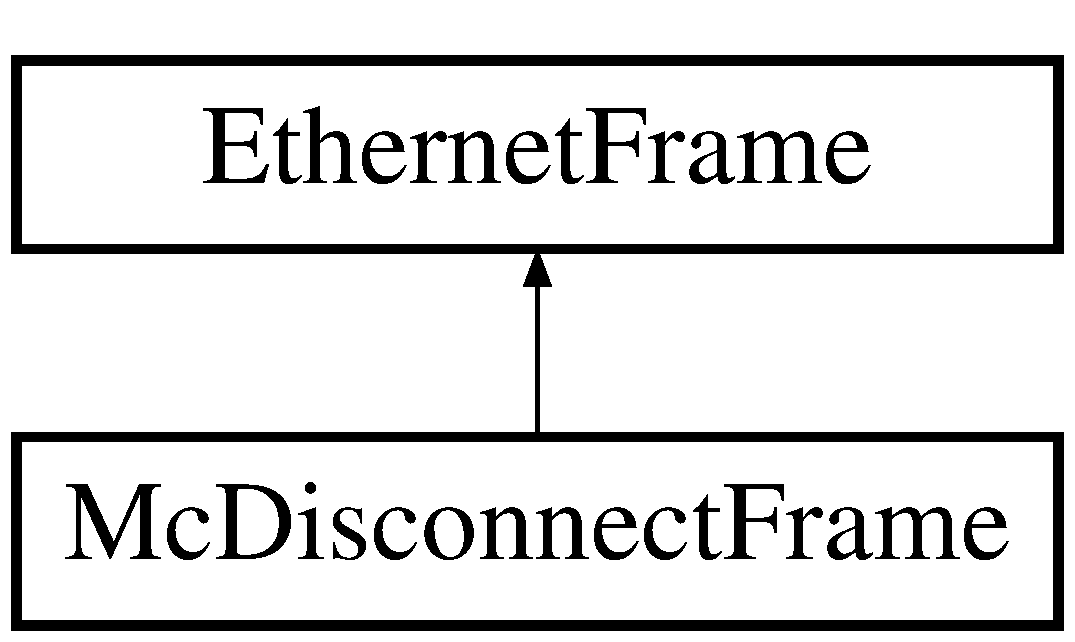
\includegraphics[height=2.000000cm]{classMcDisconnectFrame}
\end{center}
\end{figure}
\subsection*{Public Member Functions}
\begin{DoxyCompactItemize}
\item 
\hypertarget{classMcDisconnectFrame_a129496a0049d05790f8e9a3969424419}{{\bfseries Mc\-Disconnect\-Frame} (unsigned char $\ast$next\-\_\-hop, std\-::string mc\-\_\-g)}\label{classMcDisconnectFrame_a129496a0049d05790f8e9a3969424419}

\item 
\hypertarget{classMcDisconnectFrame_a0c9b7c332969140cc98f3fc6b89dca0a}{{\bfseries Mc\-Disconnect\-Frame} (unsigned char $\ast$buffer)}\label{classMcDisconnectFrame_a0c9b7c332969140cc98f3fc6b89dca0a}

\item 
\hypertarget{classMcDisconnectFrame_a8de8eef3be3247e6c49eba7ee8af774e}{std\-::string {\bfseries get\-Frame\-As\-Network\-String} (unsigned char $\ast$source)}\label{classMcDisconnectFrame_a8de8eef3be3247e6c49eba7ee8af774e}

\end{DoxyCompactItemize}
\subsection*{Data Fields}
\begin{DoxyCompactItemize}
\item 
\hypertarget{classMcDisconnectFrame_a18b0d697ab048db2933e240ccb8a0170}{struct \hyperlink{structmc__disc__header}{mc\-\_\-disc\-\_\-header} \hyperlink{classMcDisconnectFrame_a18b0d697ab048db2933e240ccb8a0170}{header\-\_\-}}\label{classMcDisconnectFrame_a18b0d697ab048db2933e240ccb8a0170}

\begin{DoxyCompactList}\small\item\em Struct which stores all fixed length header information of the Mc\-Maintenance\-Frame. \end{DoxyCompactList}\item 
\hypertarget{classMcDisconnectFrame_a87158666f709b829c6f0caf98c6e93a6}{std\-::string \hyperlink{classMcDisconnectFrame_a87158666f709b829c6f0caf98c6e93a6}{mc\-\_\-group\-\_\-}}\label{classMcDisconnectFrame_a87158666f709b829c6f0caf98c6e93a6}

\begin{DoxyCompactList}\small\item\em Name of the multicast group. \end{DoxyCompactList}\item 
\hypertarget{classMcDisconnectFrame_a1f06fd2c58ef0ed917f15a94427169f5}{bool {\bfseries disconnect\-\_\-uplink}}\label{classMcDisconnectFrame_a1f06fd2c58ef0ed917f15a94427169f5}

\item 
\hypertarget{classMcDisconnectFrame_a0487a23e5bc81fcb6b7ab854878ba828}{bool {\bfseries disconnect\-\_\-downlink}}\label{classMcDisconnectFrame_a0487a23e5bc81fcb6b7ab854878ba828}

\item 
\hypertarget{classMcDisconnectFrame_a3b4b8161f55c6f52fb280eb7c63e0ae8}{uint16\-\_\-t {\bfseries buffer\-\_\-str\-\_\-len\-\_\-}}\label{classMcDisconnectFrame_a3b4b8161f55c6f52fb280eb7c63e0ae8}

\end{DoxyCompactItemize}
\subsection*{Static Public Attributes}
\begin{DoxyCompactItemize}
\item 
\hypertarget{classMcDisconnectFrame_a08982cfea8605de09ff9f90dc62f9f46}{static uint32\-\_\-t \hyperlink{classMcDisconnectFrame_a08982cfea8605de09ff9f90dc62f9f46}{H\-E\-A\-D\-E\-R\-\_\-\-F\-I\-X\-E\-D\-\_\-\-L\-E\-N} = sizeof (\hyperlink{structeh__header}{eh\-\_\-header}) + sizeof (\hyperlink{structmc__disc__header}{mc\-\_\-disc\-\_\-header})}\label{classMcDisconnectFrame_a08982cfea8605de09ff9f90dc62f9f46}

\begin{DoxyCompactList}\small\item\em The length of the beacon header (34 bytes) \end{DoxyCompactList}\item 
\hypertarget{classMcDisconnectFrame_a3a3b299a7161d1f4e232e74c159288ba}{static uint32\-\_\-t {\bfseries stat\-\_\-id\-\_\-count} = 0}\label{classMcDisconnectFrame_a3a3b299a7161d1f4e232e74c159288ba}

\end{DoxyCompactItemize}


The documentation for this class was generated from the following files\-:\begin{DoxyCompactItemize}
\item 
src/Mc\-Disconnect\-Frame.\-h\item 
src/Mc\-Disconnect\-Frame.\-cpp\end{DoxyCompactItemize}

\hypertarget{classMcHandler}{\section{Mc\-Handler Class Reference}
\label{classMcHandler}\index{Mc\-Handler@{Mc\-Handler}}
}
\subsection*{Public Member Functions}
\begin{DoxyCompactItemize}
\item 
\hypertarget{classMcHandler_ac3dbc09dc2c3b152e87c59d9570430d8}{{\bfseries Mc\-Handler} (std\-::list$<$ \hyperlink{classMcTree}{Mc\-Tree} $\ast$ $>$ $\ast$groups)}\label{classMcHandler_ac3dbc09dc2c3b152e87c59d9570430d8}

\item 
\hypertarget{classMcHandler_a1f172f102e50907d784ffa319768ded1}{{\bfseries Mc\-Handler} (const \hyperlink{classMcHandler}{Mc\-Handler} \&orig)}\label{classMcHandler_a1f172f102e50907d784ffa319768ded1}

\item 
\hypertarget{classMcHandler_ae675a3ae1b41393e28c4850f76327212}{\hyperlink{classMcTree}{Mc\-Tree} $\ast$ {\bfseries get\-Mc\-Group} (std\-::string $\ast$group\-\_\-name)}\label{classMcHandler_ae675a3ae1b41393e28c4850f76327212}

\item 
\hypertarget{classMcHandler_aa3b39782c75c70c7eede6aed094d3099}{\hyperlink{classMcTree}{Mc\-Tree} $\ast$ {\bfseries get\-Mc\-Group} (std\-::string $\ast$hostname\-\_\-source, uint32\-\_\-t $\ast$route\-\_\-id)}\label{classMcHandler_aa3b39782c75c70c7eede6aed094d3099}

\item 
\hypertarget{classMcHandler_af2bfeebf2808b3242120efabd69ee41e}{std\-::vector$<$ \hyperlink{classMcTree}{Mc\-Tree} $\ast$ $>$ {\bfseries lost\-Connection\-Downlinks} (unsigned char $\ast$\hyperlink{structmac}{mac})}\label{classMcHandler_af2bfeebf2808b3242120efabd69ee41e}

\item 
\hypertarget{classMcHandler_a0b65a26de0e6f2376081f8f7fcd84778}{std\-::vector$<$ \hyperlink{classMcTree}{Mc\-Tree} $\ast$ $>$ {\bfseries lost\-Connection\-Uplinks} (unsigned char $\ast$\hyperlink{structmac}{mac})}\label{classMcHandler_a0b65a26de0e6f2376081f8f7fcd84778}

\item 
\hypertarget{classMcHandler_aa7ef37cbf0d5cd6eaa1d3ba6ab0e8783}{void {\bfseries create\-Group\-As\-Root} (std\-::string $\ast$group\-\_\-name)}\label{classMcHandler_aa7ef37cbf0d5cd6eaa1d3ba6ab0e8783}

\item 
\hypertarget{classMcHandler_a470f9c8360f7f57f626bad5de40489b5}{void {\bfseries add\-Group} (std\-::string $\ast$group\-\_\-name)}\label{classMcHandler_a470f9c8360f7f57f626bad5de40489b5}

\item 
\hypertarget{classMcHandler_a9d98dba49da2ef70676f1263798ed752}{bool {\bfseries add\-Uplink\-Route} (\hyperlink{structrouting__entry}{routing\-\_\-entry} $\ast$route)}\label{classMcHandler_a9d98dba49da2ef70676f1263798ed752}

\item 
\hypertarget{classMcHandler_aa84f097ecdf2b22011112dd85a1590d4}{bool {\bfseries remove\-Group} (std\-::string $\ast$group\-\_\-name)}\label{classMcHandler_aa84f097ecdf2b22011112dd85a1590d4}

\item 
\hypertarget{classMcHandler_a5b2c6085344056125d2499212b57e46a}{void {\bfseries add\-Downlink\-Route} (\hyperlink{structrouting__entry}{routing\-\_\-entry} $\ast$route)}\label{classMcHandler_a5b2c6085344056125d2499212b57e46a}

\item 
\hypertarget{classMcHandler_a831af2812933e2e5c8c90afdc3980244}{void {\bfseries set\-Membership} (std\-::string $\ast$group\-\_\-name, bool membership)}\label{classMcHandler_a831af2812933e2e5c8c90afdc3980244}

\item 
\hypertarget{classMcHandler_ac0899cc07cf9a0d588135984528659ad}{void {\bfseries print\-Mc\-Groups} ()}\label{classMcHandler_ac0899cc07cf9a0d588135984528659ad}

\end{DoxyCompactItemize}


The documentation for this class was generated from the following files\-:\begin{DoxyCompactItemize}
\item 
src/Mc\-Handler.\-h\item 
src/Mc\-Handler.\-cpp\end{DoxyCompactItemize}

\hypertarget{classMcNackFrame}{\section{Mc\-Nack\-Frame Class Reference}
\label{classMcNackFrame}\index{Mc\-Nack\-Frame@{Mc\-Nack\-Frame}}
}
Inheritance diagram for Mc\-Nack\-Frame\-:\begin{figure}[H]
\begin{center}
\leavevmode
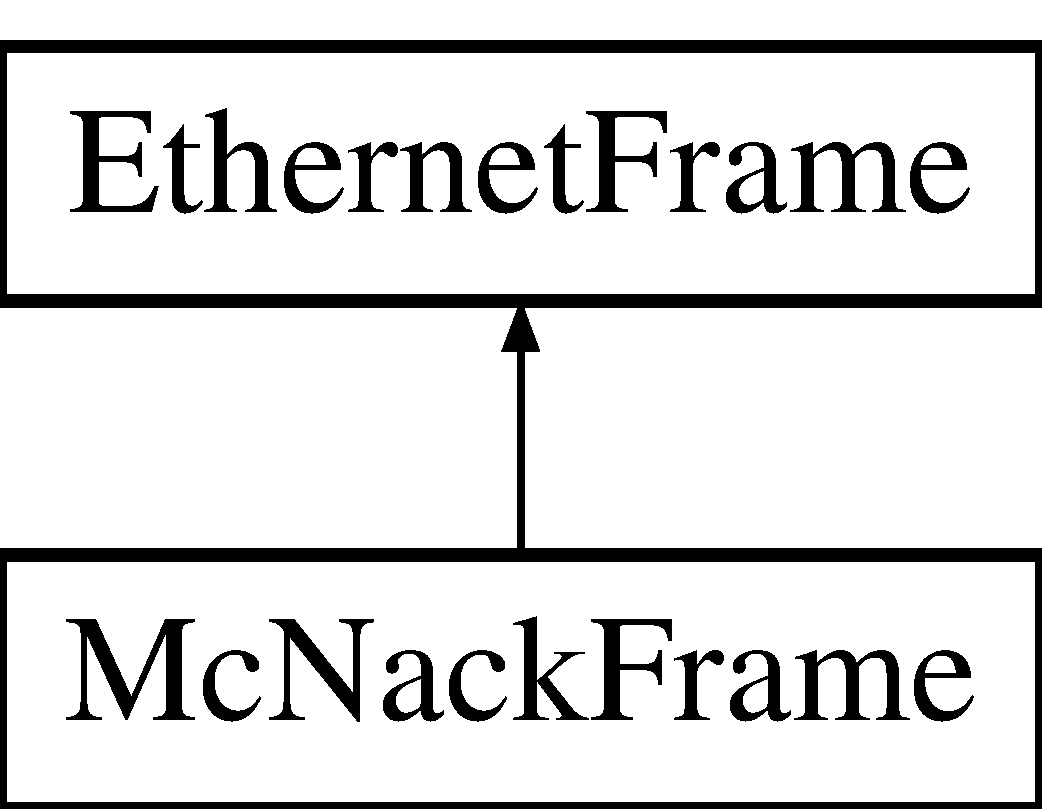
\includegraphics[height=2.000000cm]{classMcNackFrame}
\end{center}
\end{figure}
\subsection*{Public Member Functions}
\begin{DoxyCompactItemize}
\item 
\hypertarget{classMcNackFrame_af4db6b60b3850c8b77afa3370c07900f}{{\bfseries Mc\-Nack\-Frame} (unsigned char $\ast$source, unsigned char $\ast$dest, std\-::string hostname\-\_\-src, std\-::string group\-\_\-n, uint32\-\_\-t p\-\_\-id, std\-::vector$<$ uint32\-\_\-t $>$ seq\-\_\-n)}\label{classMcNackFrame_af4db6b60b3850c8b77afa3370c07900f}

\item 
\hypertarget{classMcNackFrame_a269261e2f28b1027b9f42ded34b2c550}{{\bfseries Mc\-Nack\-Frame} (unsigned char $\ast$buffer)}\label{classMcNackFrame_a269261e2f28b1027b9f42ded34b2c550}

\item 
\hypertarget{classMcNackFrame_aedae4da48bb66e40cfbf118e5843b4d7}{std\-::string {\bfseries get\-Frame\-As\-Network\-String} ()}\label{classMcNackFrame_aedae4da48bb66e40cfbf118e5843b4d7}

\item 
\hypertarget{classMcNackFrame_ad783c281cd160139a35d45764de323e9}{void {\bfseries print\-\_\-frame} ()}\label{classMcNackFrame_ad783c281cd160139a35d45764de323e9}

\end{DoxyCompactItemize}
\subsection*{Data Fields}
\begin{DoxyCompactItemize}
\item 
\hypertarget{classMcNackFrame_ad9240ce205a11535c6662039c079d3f6}{struct \hyperlink{structmc__nack__header}{mc\-\_\-nack\-\_\-header} {\bfseries header\-\_\-}}\label{classMcNackFrame_ad9240ce205a11535c6662039c079d3f6}

\item 
\hypertarget{classMcNackFrame_a01a0eea1fae23d9ea9f55934eeba0e83}{std\-::string {\bfseries hostname\-\_\-source\-\_\-}}\label{classMcNackFrame_a01a0eea1fae23d9ea9f55934eeba0e83}

\item 
\hypertarget{classMcNackFrame_a2526645198d5b6ed3668569be36e3924}{std\-::string {\bfseries mc\-\_\-group\-\_\-}}\label{classMcNackFrame_a2526645198d5b6ed3668569be36e3924}

\item 
\hypertarget{classMcNackFrame_a77e39cb742f49a02beb8089a94985336}{std\-::vector$<$ uint32\-\_\-t $>$ {\bfseries req\-\_\-seq\-\_\-nums\-\_\-}}\label{classMcNackFrame_a77e39cb742f49a02beb8089a94985336}

\item 
\hypertarget{classMcNackFrame_a99de98d91b58204785c3d3eb870dc569}{uint16\-\_\-t {\bfseries buffer\-\_\-str\-\_\-len\-\_\-}}\label{classMcNackFrame_a99de98d91b58204785c3d3eb870dc569}

\item 
\hypertarget{classMcNackFrame_a22a482caf9eedb57b67acfbd47a1b20e}{bool {\bfseries correct\-\_\-crc\-\_\-}}\label{classMcNackFrame_a22a482caf9eedb57b67acfbd47a1b20e}

\end{DoxyCompactItemize}
\subsection*{Static Public Attributes}
\begin{DoxyCompactItemize}
\item 
\hypertarget{classMcNackFrame_a65cd268403fbd386df06dc83ae38a34b}{static uint32\-\_\-t {\bfseries H\-E\-A\-D\-E\-R\-\_\-\-F\-I\-X\-E\-D\-\_\-\-L\-E\-N} = sizeof (\hyperlink{structeh__header}{eh\-\_\-header}) + sizeof (\hyperlink{structmc__nack__header}{mc\-\_\-nack\-\_\-header})}\label{classMcNackFrame_a65cd268403fbd386df06dc83ae38a34b}

\item 
\hypertarget{classMcNackFrame_aac54da745331453c3c3c629df8764dc8}{static uint32\-\_\-t {\bfseries stat\-\_\-id\-\_\-count} = 0}\label{classMcNackFrame_aac54da745331453c3c3c629df8764dc8}

\end{DoxyCompactItemize}


The documentation for this class was generated from the following files\-:\begin{DoxyCompactItemize}
\item 
src/Mc\-Nack\-Frame.\-h\item 
src/Mc\-Nack\-Frame.\-cpp\end{DoxyCompactItemize}

\hypertarget{classMcPosAckObj}{\section{Mc\-Pos\-Ack\-Obj Class Reference}
\label{classMcPosAckObj}\index{Mc\-Pos\-Ack\-Obj@{Mc\-Pos\-Ack\-Obj}}
}
\subsection*{Public Member Functions}
\begin{DoxyCompactItemize}
\item 
\hypertarget{classMcPosAckObj_aa63ad2946065ff26a78671109af67ca8}{{\bfseries Mc\-Pos\-Ack\-Obj} (\hyperlink{classRoutedFrame}{Routed\-Frame} $\ast$frame, \hyperlink{classMcTree}{Mc\-Tree} $\ast$group)}\label{classMcPosAckObj_aa63ad2946065ff26a78671109af67ca8}

\item 
\hypertarget{classMcPosAckObj_a9c1f1e33883f308f0ccad7ddf2b044a1}{{\bfseries Mc\-Pos\-Ack\-Obj} (const \hyperlink{classMcPosAckObj}{Mc\-Pos\-Ack\-Obj} \&orig)}\label{classMcPosAckObj_a9c1f1e33883f308f0ccad7ddf2b044a1}

\item 
\hypertarget{classMcPosAckObj_a747dfe74d820a1dbc08732c82d79c85e}{bool {\bfseries Got\-Ack} (\hyperlink{classMcAckFrame}{Mc\-Ack\-Frame} $\ast$ack)}\label{classMcPosAckObj_a747dfe74d820a1dbc08732c82d79c85e}

\end{DoxyCompactItemize}
\subsection*{Data Fields}
\begin{DoxyCompactItemize}
\item 
\hypertarget{classMcPosAckObj_ad909900f199558f70262cb253bb9294d}{std\-::list$<$ unsigned char $\ast$ $>$ {\bfseries missing\-\_\-acks\-\_\-l}}\label{classMcPosAckObj_ad909900f199558f70262cb253bb9294d}

\item 
\hypertarget{classMcPosAckObj_a8d7afb2c0a16577e604a7e39d55fcb9a}{unsigned char $\ast$ {\bfseries incoming\-\_\-mac}}\label{classMcPosAckObj_a8d7afb2c0a16577e604a7e39d55fcb9a}

\item 
\hypertarget{classMcPosAckObj_acc1cf85260df78347cc24613bca1070e}{std\-::string {\bfseries group\-\_\-name}}\label{classMcPosAckObj_acc1cf85260df78347cc24613bca1070e}

\item 
\hypertarget{classMcPosAckObj_a45476d77f496bf607b7a3e0fe077fa9c}{uint32\-\_\-t {\bfseries sequence\-\_\-num}}\label{classMcPosAckObj_a45476d77f496bf607b7a3e0fe077fa9c}

\item 
\hypertarget{classMcPosAckObj_aa49ed639148f2b70a6b0e5893f2f36b7}{uint32\-\_\-t {\bfseries packet\-\_\-id}}\label{classMcPosAckObj_aa49ed639148f2b70a6b0e5893f2f36b7}

\end{DoxyCompactItemize}


The documentation for this class was generated from the following files\-:\begin{DoxyCompactItemize}
\item 
src/Mc\-Pos\-Ack\-Obj.\-h\item 
src/Mc\-Pos\-Ack\-Obj.\-cpp\end{DoxyCompactItemize}

\hypertarget{classMcRouteActivationFrame}{\section{Mc\-Route\-Activation\-Frame Class Reference}
\label{classMcRouteActivationFrame}\index{Mc\-Route\-Activation\-Frame@{Mc\-Route\-Activation\-Frame}}
}
Inheritance diagram for Mc\-Route\-Activation\-Frame\-:\begin{figure}[H]
\begin{center}
\leavevmode
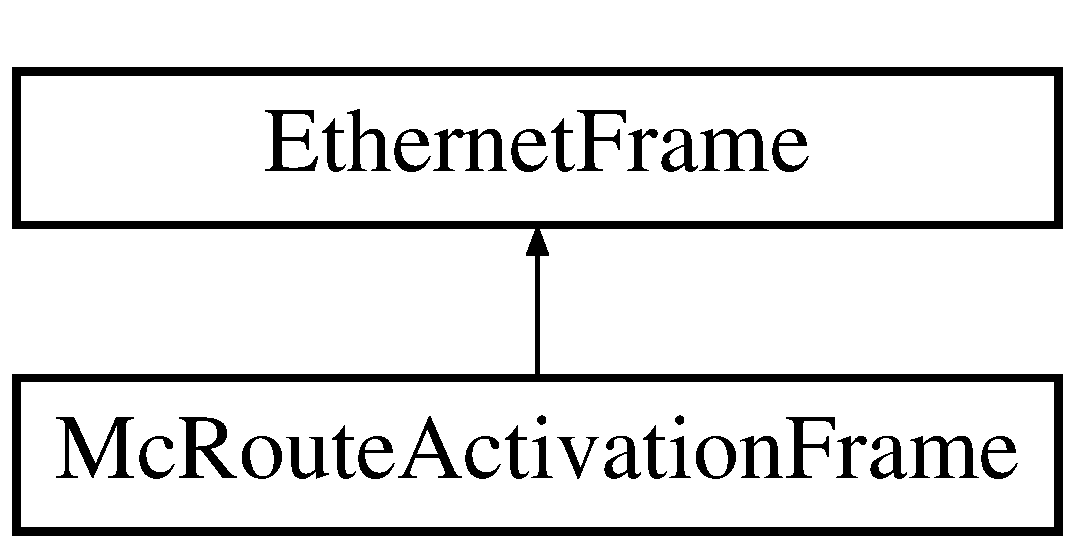
\includegraphics[height=2.000000cm]{classMcRouteActivationFrame}
\end{center}
\end{figure}
\subsection*{Public Member Functions}
\begin{DoxyCompactItemize}
\item 
\hyperlink{classMcRouteActivationFrame_a2a6ad3848eb8318aa6eb332552cc4f9a}{Mc\-Route\-Activation\-Frame} (unsigned char $\ast$next\-\_\-hop, std\-::string mc\-\_\-g, uint32\-\_\-t route\-\_\-id, std\-::string source)
\begin{DoxyCompactList}\small\item\em Constructs the Mc\-Maintenance\-Frame on the sender side. \end{DoxyCompactList}\item 
\hyperlink{classMcRouteActivationFrame_af5a50874d6ad2a5c28546fff47b5f35b}{Mc\-Route\-Activation\-Frame} (unsigned char $\ast$buffer)
\begin{DoxyCompactList}\small\item\em Constructs the Mc\-Maintenance\-Frame on the receiver side. \end{DoxyCompactList}\item 
std\-::string \hyperlink{classMcRouteActivationFrame_ad06e4b44308c0bdc6af1709665ecf4bf}{get\-Frame\-As\-Network\-String} (unsigned char source\mbox{[}6\mbox{]})
\begin{DoxyCompactList}\small\item\em Returns a Mc\-Maintenance\-Frame as a C++ string. \end{DoxyCompactList}\end{DoxyCompactItemize}
\subsection*{Data Fields}
\begin{DoxyCompactItemize}
\item 
\hypertarget{classMcRouteActivationFrame_a40acfccedd076c1be9f923a8f4dbee78}{struct \hyperlink{structmc__act__header}{mc\-\_\-act\-\_\-header} \hyperlink{classMcRouteActivationFrame_a40acfccedd076c1be9f923a8f4dbee78}{header\-\_\-}}\label{classMcRouteActivationFrame_a40acfccedd076c1be9f923a8f4dbee78}

\begin{DoxyCompactList}\small\item\em Struct which stores all fixed length header information of the Mc\-Maintenance\-Frame. \end{DoxyCompactList}\item 
\hypertarget{classMcRouteActivationFrame_a5e542ea32c6d081c567ecae45b5f1412}{std\-::string \hyperlink{classMcRouteActivationFrame_a5e542ea32c6d081c567ecae45b5f1412}{mc\-\_\-group\-\_\-}}\label{classMcRouteActivationFrame_a5e542ea32c6d081c567ecae45b5f1412}

\begin{DoxyCompactList}\small\item\em Name of the multicast group. \end{DoxyCompactList}\item 
\hypertarget{classMcRouteActivationFrame_a81d1b380baec0e1f99972fadc1850643}{std\-::string \hyperlink{classMcRouteActivationFrame_a81d1b380baec0e1f99972fadc1850643}{hostname\-\_\-source\-\_\-}}\label{classMcRouteActivationFrame_a81d1b380baec0e1f99972fadc1850643}

\begin{DoxyCompactList}\small\item\em Name of the multicast group. \end{DoxyCompactList}\item 
\hypertarget{classMcRouteActivationFrame_aedadc5847e3cfa92f24aef02b019c5f1}{uint16\-\_\-t {\bfseries buffer\-\_\-str\-\_\-len\-\_\-}}\label{classMcRouteActivationFrame_aedadc5847e3cfa92f24aef02b019c5f1}

\end{DoxyCompactItemize}
\subsection*{Static Public Attributes}
\begin{DoxyCompactItemize}
\item 
\hypertarget{classMcRouteActivationFrame_a73efc6b0a072676334b1a1336bf121b2}{static uint32\-\_\-t \hyperlink{classMcRouteActivationFrame_a73efc6b0a072676334b1a1336bf121b2}{H\-E\-A\-D\-E\-R\-\_\-\-F\-I\-X\-E\-D\-\_\-\-L\-E\-N} = sizeof (\hyperlink{structeh__header}{eh\-\_\-header}) + sizeof (\hyperlink{structmc__act__header}{mc\-\_\-act\-\_\-header})}\label{classMcRouteActivationFrame_a73efc6b0a072676334b1a1336bf121b2}

\begin{DoxyCompactList}\small\item\em The length of the beacon header (34 bytes) \end{DoxyCompactList}\item 
\hypertarget{classMcRouteActivationFrame_a768920bc0f5d945068dc85ab3d3c8747}{static uint32\-\_\-t {\bfseries stat\-\_\-id\-\_\-count} = 0}\label{classMcRouteActivationFrame_a768920bc0f5d945068dc85ab3d3c8747}

\end{DoxyCompactItemize}


\subsection{Constructor \& Destructor Documentation}
\hypertarget{classMcRouteActivationFrame_a2a6ad3848eb8318aa6eb332552cc4f9a}{\index{Mc\-Route\-Activation\-Frame@{Mc\-Route\-Activation\-Frame}!Mc\-Route\-Activation\-Frame@{Mc\-Route\-Activation\-Frame}}
\index{Mc\-Route\-Activation\-Frame@{Mc\-Route\-Activation\-Frame}!McRouteActivationFrame@{Mc\-Route\-Activation\-Frame}}
\subsubsection[{Mc\-Route\-Activation\-Frame}]{\setlength{\rightskip}{0pt plus 5cm}Mc\-Route\-Activation\-Frame\-::\-Mc\-Route\-Activation\-Frame (
\begin{DoxyParamCaption}
\item[{unsigned char $\ast$}]{next\-\_\-hop, }
\item[{std\-::string}]{mc\-\_\-g, }
\item[{uint32\-\_\-t}]{route\-\_\-id, }
\item[{std\-::string}]{source}
\end{DoxyParamCaption}
)}}\label{classMcRouteActivationFrame_a2a6ad3848eb8318aa6eb332552cc4f9a}


Constructs the Mc\-Maintenance\-Frame on the sender side. 


\begin{DoxyParams}{Parameters}
{\em route} & The route the frame will take \\
\hline
{\em activate\textbackslash{}xrefitem} & todo 1. \\
\hline
\end{DoxyParams}
\hypertarget{classMcRouteActivationFrame_af5a50874d6ad2a5c28546fff47b5f35b}{\index{Mc\-Route\-Activation\-Frame@{Mc\-Route\-Activation\-Frame}!Mc\-Route\-Activation\-Frame@{Mc\-Route\-Activation\-Frame}}
\index{Mc\-Route\-Activation\-Frame@{Mc\-Route\-Activation\-Frame}!McRouteActivationFrame@{Mc\-Route\-Activation\-Frame}}
\subsubsection[{Mc\-Route\-Activation\-Frame}]{\setlength{\rightskip}{0pt plus 5cm}Mc\-Route\-Activation\-Frame\-::\-Mc\-Route\-Activation\-Frame (
\begin{DoxyParamCaption}
\item[{unsigned char $\ast$}]{buffer}
\end{DoxyParamCaption}
)}}\label{classMcRouteActivationFrame_af5a50874d6ad2a5c28546fff47b5f35b}


Constructs the Mc\-Maintenance\-Frame on the receiver side. 


\begin{DoxyParams}{Parameters}
{\em buffer} & The received network buffer \\
\hline
\end{DoxyParams}


\subsection{Member Function Documentation}
\hypertarget{classMcRouteActivationFrame_ad06e4b44308c0bdc6af1709665ecf4bf}{\index{Mc\-Route\-Activation\-Frame@{Mc\-Route\-Activation\-Frame}!get\-Frame\-As\-Network\-String@{get\-Frame\-As\-Network\-String}}
\index{get\-Frame\-As\-Network\-String@{get\-Frame\-As\-Network\-String}!McRouteActivationFrame@{Mc\-Route\-Activation\-Frame}}
\subsubsection[{get\-Frame\-As\-Network\-String}]{\setlength{\rightskip}{0pt plus 5cm}std\-::string Mc\-Route\-Activation\-Frame\-::get\-Frame\-As\-Network\-String (
\begin{DoxyParamCaption}
\item[{unsigned char}]{source\mbox{[}6\mbox{]}}
\end{DoxyParamCaption}
)}}\label{classMcRouteActivationFrame_ad06e4b44308c0bdc6af1709665ecf4bf}


Returns a Mc\-Maintenance\-Frame as a C++ string. 

Converts the Maintenence\-Frame into a C++ string to be written to the socket. \begin{DoxyReturn}{Returns}
Mc\-Maintenance\-Frame as C++ string. 
\end{DoxyReturn}


The documentation for this class was generated from the following files\-:\begin{DoxyCompactItemize}
\item 
src/Mc\-Route\-Activation\-Frame.\-h\item 
src/Mc\-Route\-Activation\-Frame.\-cpp\end{DoxyCompactItemize}

\hypertarget{classMcTree}{\section{Mc\-Tree Class Reference}
\label{classMcTree}\index{Mc\-Tree@{Mc\-Tree}}
}
\subsection*{Public Member Functions}
\begin{DoxyCompactItemize}
\item 
\hypertarget{classMcTree_ae6e7ec5f80ed5cabcfe6383dfd77fdcd}{{\bfseries Mc\-Tree} (const \hyperlink{classMcTree}{Mc\-Tree} \&orig)}\label{classMcTree_ae6e7ec5f80ed5cabcfe6383dfd77fdcd}

\item 
\hypertarget{classMcTree_a44a8bca5229a33b3956f02b698d8d4e4}{bool {\bfseries activate\-Best\-Route} (\hyperlink{structroute__request}{route\-\_\-request} $\ast$rreq\-\_\-logging)}\label{classMcTree_a44a8bca5229a33b3956f02b698d8d4e4}

\item 
\hypertarget{classMcTree_ae90b832fbebc0acf66556f2d0e2adb84}{bool {\bfseries activate\-Route} (std\-::string $\ast$hostname\-\_\-source, uint32\-\_\-t $\ast$id, unsigned char $\ast$mac\-\_\-adr)}\label{classMcTree_ae90b832fbebc0acf66556f2d0e2adb84}

\item 
\hypertarget{classMcTree_a609138636cf6f77d902d571e28c07d88}{bool {\bfseries route\-Is\-New} (\hyperlink{structrouting__entry}{routing\-\_\-entry} $\ast$r)}\label{classMcTree_a609138636cf6f77d902d571e28c07d88}

\item 
\hypertarget{classMcTree_a74b698d094e8c2965f39bbf02d417329}{bool {\bfseries process\-Frame} (unsigned char $\ast$src)}\label{classMcTree_a74b698d094e8c2965f39bbf02d417329}

\item 
\hypertarget{classMcTree_ab374ea31c27bb6441ffd24650d52542f}{bool {\bfseries add\-Downlink\-As\-Member} (\hyperlink{structmac}{mac} $\ast$m)}\label{classMcTree_ab374ea31c27bb6441ffd24650d52542f}

\item 
\hypertarget{classMcTree_ab1203d62a3530db8d38cbcf83cdaff7f}{bool {\bfseries add\-Downlink\-As\-Connector} (\hyperlink{structmac}{mac} $\ast$m)}\label{classMcTree_ab1203d62a3530db8d38cbcf83cdaff7f}

\item 
\hypertarget{classMcTree_a2a683aa8a1cdab2f3d28046608f49694}{bool {\bfseries add\-Waiting\-Request} (\hyperlink{classRouteRequest}{Route\-Request} $\ast$req, unsigned char $\ast$source\-\_\-mac)}\label{classMcTree_a2a683aa8a1cdab2f3d28046608f49694}

\item 
\hypertarget{classMcTree_acee7fd958591ea6a7bb1cfed4a166812}{bool {\bfseries propagate\-Frame} (unsigned char $\ast$sender\-\_\-mac)}\label{classMcTree_acee7fd958591ea6a7bb1cfed4a166812}

\item 
\hypertarget{classMcTree_a68de6f320a8900bee7cd1a17ba608778}{void {\bfseries safe\-Outgoing\-Request} (\hyperlink{classRouteRequest}{Route\-Request} $\ast$req)}\label{classMcTree_a68de6f320a8900bee7cd1a17ba608778}

\item 
\hypertarget{classMcTree_ac7a21fd806fa9c0c825d0c9e2f6037cc}{void {\bfseries reset\-Tmp\-Fields} ()}\label{classMcTree_ac7a21fd806fa9c0c825d0c9e2f6037cc}

\item 
\hypertarget{classMcTree_a4e627637f66a8a2768036245e8fe7a1b}{bool {\bfseries downlink\-Exsists} (unsigned char $\ast$m)}\label{classMcTree_a4e627637f66a8a2768036245e8fe7a1b}

\item 
\hypertarget{classMcTree_ae4596d618fba858d96441701b95286dc}{bool {\bfseries remove\-Mac\-If\-Exsists} (unsigned char $\ast$m)}\label{classMcTree_ae4596d618fba858d96441701b95286dc}

\item 
\hypertarget{classMcTree_a5fcf06613c9e3b5e3d007750d85d957d}{void {\bfseries print\-Tree} ()}\label{classMcTree_a5fcf06613c9e3b5e3d007750d85d957d}

\item 
\hypertarget{classMcTree_ac81005763adb448558d664e36e512ecf}{bool {\bfseries operator=} (const \hyperlink{classMcTree}{Mc\-Tree} $\ast$other)}\label{classMcTree_ac81005763adb448558d664e36e512ecf}

\end{DoxyCompactItemize}
\subsection*{Data Fields}
\begin{DoxyCompactItemize}
\item 
\hypertarget{classMcTree_a0c1d0f05e3e15a1e2f34da89af60b7b6}{std\-::string {\bfseries group\-\_\-name\-\_\-}}\label{classMcTree_a0c1d0f05e3e15a1e2f34da89af60b7b6}

\item 
\hypertarget{classMcTree_a9981a01e6a0dba10df1410180185f68f}{\hyperlink{structrouting__entry}{routing\-\_\-entry} $\ast$ {\bfseries route\-\_\-uplink\-\_\-}}\label{classMcTree_a9981a01e6a0dba10df1410180185f68f}

\item 
\hypertarget{classMcTree_a30035023d97348916ee6e96bff2dfeec}{\hyperlink{classRouteRequest}{Route\-Request} $\ast$ {\bfseries outgoing\-\_\-request\-\_\-}}\label{classMcTree_a30035023d97348916ee6e96bff2dfeec}

\item 
\hypertarget{classMcTree_a42b5e7daf64fab9087f3583e342da5be}{std\-::list$<$ \hyperlink{structmac}{mac} $\ast$ $>$ {\bfseries downlinks\-\_\-l\-\_\-}}\label{classMcTree_a42b5e7daf64fab9087f3583e342da5be}

\item 
\hypertarget{classMcTree_ad8608e35630eb3039d30c237943f06e1}{unsigned long {\bfseries time\-\_\-stamp\-\_\-}}\label{classMcTree_ad8608e35630eb3039d30c237943f06e1}

\item 
\hypertarget{classMcTree_a429e63decbf8d5392120645a4a32a407}{std\-::list$<$ \hyperlink{classRouteRequest}{Route\-Request} $\ast$ $>$ {\bfseries waiting\-\_\-requests\-\_\-l\-\_\-}}\label{classMcTree_a429e63decbf8d5392120645a4a32a407}

\item 
\hypertarget{classMcTree_ae15d457bf08d64befaaaefd70eac31fb}{std\-::list$<$ \hyperlink{structrouting__entry}{routing\-\_\-entry} $\ast$ $>$ {\bfseries routing\-\_\-entries\-\_\-l\-\_\-}}\label{classMcTree_ae15d457bf08d64befaaaefd70eac31fb}

\item 
\hypertarget{classMcTree_a525e7fa1646f961a5f07f22e9316e537}{std\-::list$<$ \hyperlink{structrouting__entry}{routing\-\_\-entry} $\ast$ $>$ {\bfseries routing\-\_\-entries\-\_\-downlinks\-\_\-l\-\_\-}}\label{classMcTree_a525e7fa1646f961a5f07f22e9316e537}

\item 
\hypertarget{classMcTree_a0ac20f71cbb9a85d56ee3224baaa828c}{bool {\bfseries member}}\label{classMcTree_a0ac20f71cbb9a85d56ee3224baaa828c}

\item 
\hypertarget{classMcTree_ae71202567a76e8f7c5090e6d88b9f7bb}{bool {\bfseries activated}}\label{classMcTree_ae71202567a76e8f7c5090e6d88b9f7bb}

\item 
\hypertarget{classMcTree_a95aed3d5f4b4462d9eefe395aae682f6}{bool {\bfseries connected}}\label{classMcTree_a95aed3d5f4b4462d9eefe395aae682f6}

\item 
\hypertarget{classMcTree_aca22645aa04356858acb0a8c7aae5b8c}{bool {\bfseries root}}\label{classMcTree_aca22645aa04356858acb0a8c7aae5b8c}

\end{DoxyCompactItemize}


The documentation for this class was generated from the following files\-:\begin{DoxyCompactItemize}
\item 
src/Mc\-Tree.\-h\item 
src/Mc\-Tree.\-cpp\end{DoxyCompactItemize}

\hypertarget{structmh__bcast__header}{\section{mh\-\_\-bcast\-\_\-header Struct Reference}
\label{structmh__bcast__header}\index{mh\-\_\-bcast\-\_\-header@{mh\-\_\-bcast\-\_\-header}}
}
\subsection*{Data Fields}
\begin{DoxyCompactItemize}
\item 
\hypertarget{structmh__bcast__header_a645bc6e0f599ba87f09b808c7d132d68}{uint8\-\_\-t {\bfseries frame\-\_\-type}}\label{structmh__bcast__header_a645bc6e0f599ba87f09b808c7d132d68}

\item 
\hypertarget{structmh__bcast__header_aae2a3d39f8f9fa5b357e9689bc4d170c}{uint32\-\_\-t {\bfseries id}}\label{structmh__bcast__header_aae2a3d39f8f9fa5b357e9689bc4d170c}

\item 
\hypertarget{structmh__bcast__header_af389a933a7cd120045ff9241258b9eb6}{uint8\-\_\-t {\bfseries payload\-\_\-type}}\label{structmh__bcast__header_af389a933a7cd120045ff9241258b9eb6}

\item 
\hypertarget{structmh__bcast__header_aa6a1428ebcbe730f935205bdbbb3ed63}{uint16\-\_\-t {\bfseries current\-\_\-hop}}\label{structmh__bcast__header_aa6a1428ebcbe730f935205bdbbb3ed63}

\item 
\hypertarget{structmh__bcast__header_a7554ca13a6890da26c5fb5d1f31550ea}{uint16\-\_\-t {\bfseries hop\-\_\-limit}}\label{structmh__bcast__header_a7554ca13a6890da26c5fb5d1f31550ea}

\item 
\hypertarget{structmh__bcast__header_ad9b04518fb7586258e0e9bb73a5f0275}{uint32\-\_\-t {\bfseries hostname\-\_\-source\-\_\-len}}\label{structmh__bcast__header_ad9b04518fb7586258e0e9bb73a5f0275}

\item 
\hypertarget{structmh__bcast__header_a7999a82698db4ab8b7da051d5546427e}{uint32\-\_\-t {\bfseries topic\-\_\-len}}\label{structmh__bcast__header_a7999a82698db4ab8b7da051d5546427e}

\item 
\hypertarget{structmh__bcast__header_a2afe2d8d8e3616e060718af5743b3dc7}{uint32\-\_\-t {\bfseries payload\-\_\-len}}\label{structmh__bcast__header_a2afe2d8d8e3616e060718af5743b3dc7}

\end{DoxyCompactItemize}


The documentation for this struct was generated from the following file\-:\begin{DoxyCompactItemize}
\item 
src/Multi\-Hop\-Broadcast\-Frame.\-h\end{DoxyCompactItemize}

\hypertarget{classMultiHopBroadcastFrame}{\section{Multi\-Hop\-Broadcast\-Frame Class Reference}
\label{classMultiHopBroadcastFrame}\index{Multi\-Hop\-Broadcast\-Frame@{Multi\-Hop\-Broadcast\-Frame}}
}
Inheritance diagram for Multi\-Hop\-Broadcast\-Frame\-:\begin{figure}[H]
\begin{center}
\leavevmode
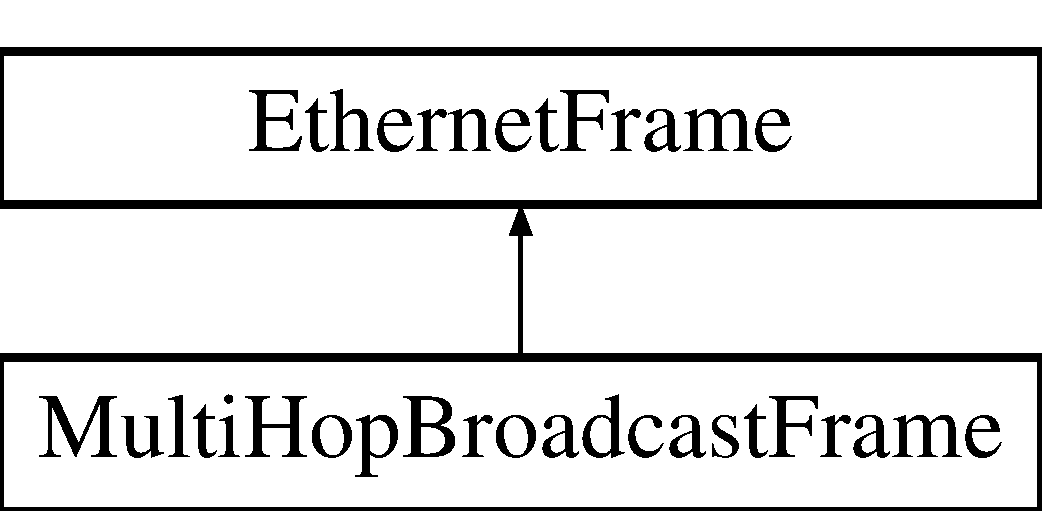
\includegraphics[height=2.000000cm]{classMultiHopBroadcastFrame}
\end{center}
\end{figure}
\subsection*{Public Member Functions}
\begin{DoxyCompactItemize}
\item 
\hypertarget{classMultiHopBroadcastFrame_a0d3aaa1aff406a09aba58d5a3de3d24e}{{\bfseries Multi\-Hop\-Broadcast\-Frame} (std\-::string topic\-\_\-to\-\_\-publish, std\-::string data, string source\-\_\-host, uint8\-\_\-t payload\-\_\-type\-\_\-field, uint16\-\_\-t hop\-\_\-range)}\label{classMultiHopBroadcastFrame_a0d3aaa1aff406a09aba58d5a3de3d24e}

\item 
\hypertarget{classMultiHopBroadcastFrame_a44124c28205fae156e4107763cd6a0a8}{{\bfseries Multi\-Hop\-Broadcast\-Frame} (unsigned char $\ast$buffer)}\label{classMultiHopBroadcastFrame_a44124c28205fae156e4107763cd6a0a8}

\item 
\hypertarget{classMultiHopBroadcastFrame_a4dad86835ff3d79ba9462e030ae019c9}{std\-::string {\bfseries get\-Frame\-As\-Network\-String} (unsigned char $\ast$source)}\label{classMultiHopBroadcastFrame_a4dad86835ff3d79ba9462e030ae019c9}

\end{DoxyCompactItemize}
\subsection*{Data Fields}
\begin{DoxyCompactItemize}
\item 
\hypertarget{classMultiHopBroadcastFrame_af3386512fd14333945a2880d56a49050}{bool {\bfseries rebroadcast}}\label{classMultiHopBroadcastFrame_af3386512fd14333945a2880d56a49050}

\item 
\hypertarget{classMultiHopBroadcastFrame_aa0908ec720cf4b166d8241bbeda3ef72}{struct \hyperlink{structmh__bcast__header}{mh\-\_\-bcast\-\_\-header} {\bfseries header\-\_\-}}\label{classMultiHopBroadcastFrame_aa0908ec720cf4b166d8241bbeda3ef72}

\item 
\hypertarget{classMultiHopBroadcastFrame_a74ca707efb4010d99e5fedc2c0139b7e}{uint16\-\_\-t {\bfseries buffer\-\_\-str\-\_\-len\-\_\-}}\label{classMultiHopBroadcastFrame_a74ca707efb4010d99e5fedc2c0139b7e}

\item 
\hypertarget{classMultiHopBroadcastFrame_ac02d0f6c484c46b61306308a37a24ea2}{std\-::string {\bfseries hostname\-\_\-source\-\_\-}}\label{classMultiHopBroadcastFrame_ac02d0f6c484c46b61306308a37a24ea2}

\item 
\hypertarget{classMultiHopBroadcastFrame_aab544fda0811d4003524c23299390ecf}{std\-::string {\bfseries topic\-\_\-}}\label{classMultiHopBroadcastFrame_aab544fda0811d4003524c23299390ecf}

\item 
\hypertarget{classMultiHopBroadcastFrame_a52f9b2799c52d49cf8ee0cea737de234}{std\-::string {\bfseries payload\-\_\-}}\label{classMultiHopBroadcastFrame_a52f9b2799c52d49cf8ee0cea737de234}

\end{DoxyCompactItemize}
\subsection*{Static Public Attributes}
\begin{DoxyCompactItemize}
\item 
\hypertarget{classMultiHopBroadcastFrame_a4db937c772e736c50aca80727128310a}{static uint32\-\_\-t {\bfseries frame\-\_\-count\-\_\-stat} = 0}\label{classMultiHopBroadcastFrame_a4db937c772e736c50aca80727128310a}

\item 
\hypertarget{classMultiHopBroadcastFrame_a502ee128ede8ca2bcb30c18243daee8f}{static uint32\-\_\-t {\bfseries H\-E\-A\-D\-E\-R\-\_\-\-F\-I\-X\-E\-D\-\_\-\-L\-E\-N} = sizeof (\hyperlink{structeh__header}{eh\-\_\-header}) + sizeof (\hyperlink{structmh__bcast__header}{mh\-\_\-bcast\-\_\-header})}\label{classMultiHopBroadcastFrame_a502ee128ede8ca2bcb30c18243daee8f}

\end{DoxyCompactItemize}


The documentation for this class was generated from the following files\-:\begin{DoxyCompactItemize}
\item 
src/Multi\-Hop\-Broadcast\-Frame.\-h\item 
src/Multi\-Hop\-Broadcast\-Frame.\-cpp\end{DoxyCompactItemize}

\hypertarget{classPacket}{\section{Packet Class Reference}
\label{classPacket}\index{Packet@{Packet}}
}


The packet class for network layer packets.  




{\ttfamily \#include $<$Packet.\-h$>$}

\subsection*{Public Member Functions}
\begin{DoxyCompactItemize}
\item 
\hyperlink{classPacket_ac9c69d1e86e52f896ba5392b57baa7f6}{Packet} (\hyperlink{classRoutedFrame}{Routed\-Frame} frame)
\begin{DoxyCompactList}\small\item\em \hyperlink{classPacket}{Packet} constructor. \end{DoxyCompactList}\item 
\hypertarget{classPacket_ad70f0a6e94787200b33a651f559aeaab}{bool {\bfseries frame\-Already\-Exsits} (\hyperlink{classRoutedFrame}{Routed\-Frame} f)}\label{classPacket_ad70f0a6e94787200b33a651f559aeaab}

\item 
\hypertarget{classPacket_acc003fd8ca771e7c76689871138f4d51}{void {\bfseries refresh\-Lists} ()}\label{classPacket_acc003fd8ca771e7c76689871138f4d51}

\item 
\hypertarget{classPacket_a44ae78eb4f5acef68fdbe61d357d1956}{void {\bfseries sort\-Frame\-List} ()}\label{classPacket_a44ae78eb4f5acef68fdbe61d357d1956}

\item 
\hypertarget{classPacket_a94ff1e02094fcf7c4227610415b60352}{unsigned long {\bfseries get\-Size} ()}\label{classPacket_a94ff1e02094fcf7c4227610415b60352}

\item 
\hypertarget{classPacket_acb764ed00dc608bf08e0b6fa1e1406fa}{void {\bfseries request\-Missing\-Frames} ()}\label{classPacket_acb764ed00dc608bf08e0b6fa1e1406fa}

\item 
\hypertarget{classPacket_a8d2267ee0e2e29c14a474e11b0f504c4}{void {\bfseries refresh\-Missing\-Frames\-List} ()}\label{classPacket_a8d2267ee0e2e29c14a474e11b0f504c4}

\item 
bool \hyperlink{classPacket_a0abfc59341b18a0b3830522fd344579c}{add\-Frame} (\hyperlink{classRoutedFrame}{Routed\-Frame} frame)
\begin{DoxyCompactList}\small\item\em Add the frame to the frame list of the packet, if the frame belongs to the packet. \end{DoxyCompactList}\item 
\hypertarget{classPacket_a365c5a9500b374b8fb3f2c8806523647}{bool {\bfseries is\-Mc\-Frame} ()}\label{classPacket_a365c5a9500b374b8fb3f2c8806523647}

\item 
\hypertarget{classPacket_ae1349ae330ed8943436e24ed7d6d2f02}{bool {\bfseries is\-Nack} ()}\label{classPacket_ae1349ae330ed8943436e24ed7d6d2f02}

\item 
std\-::string \hyperlink{classPacket_aeff54aea0863db044a2948d38895e8aa}{get\-Payload} ()
\begin{DoxyCompactList}\small\item\em Returns the packet's payload. \end{DoxyCompactList}\end{DoxyCompactItemize}
\subsection*{Data Fields}
\begin{DoxyCompactItemize}
\item 
\hypertarget{classPacket_a037d2ae2061811448165d1e414f9c5ed}{uint32\-\_\-t \hyperlink{classPacket_a037d2ae2061811448165d1e414f9c5ed}{id\-\_\-}}\label{classPacket_a037d2ae2061811448165d1e414f9c5ed}

\begin{DoxyCompactList}\small\item\em \hyperlink{classPacket}{Packet} I\-D. \end{DoxyCompactList}\item 
\hypertarget{classPacket_a20475a5c401177fa680e35d9c7d75379}{uint32\-\_\-t {\bfseries highest\-\_\-seq}}\label{classPacket_a20475a5c401177fa680e35d9c7d75379}

\item 
\hypertarget{classPacket_a8dad90df4b1877a240d2b8397a703665}{uint32\-\_\-t \hyperlink{classPacket_a8dad90df4b1877a240d2b8397a703665}{size\-\_\-}}\label{classPacket_a8dad90df4b1877a240d2b8397a703665}

\begin{DoxyCompactList}\small\item\em Size of packet in bytes. \end{DoxyCompactList}\item 
uint8\-\_\-t \hyperlink{classPacket_a6eee220fed8f687022dde8c2a162080e}{data\-\_\-type\-\_\-}
\item 
\hypertarget{classPacket_ad7cf180de7010296b3fe562cf2f407b6}{bool {\bfseries wrong\-\_\-sequence\-\_\-}}\label{classPacket_ad7cf180de7010296b3fe562cf2f407b6}

\item 
\hypertarget{classPacket_ab4ff4a240a31a7c14621651e66a760b7}{std\-::string \hyperlink{classPacket_ab4ff4a240a31a7c14621651e66a760b7}{hostname\-\_\-source\-\_\-}}\label{classPacket_ab4ff4a240a31a7c14621651e66a760b7}

\begin{DoxyCompactList}\small\item\em hostname of the source \end{DoxyCompactList}\item 
\hypertarget{classPacket_aee88f59c3815270859141bd3a0d6e1b2}{std\-::string \hyperlink{classPacket_aee88f59c3815270859141bd3a0d6e1b2}{mc\-\_\-group\-\_\-}}\label{classPacket_aee88f59c3815270859141bd3a0d6e1b2}

\begin{DoxyCompactList}\small\item\em name of the mc group \end{DoxyCompactList}\item 
\hypertarget{classPacket_ae7e1f61be22aa9b212c7346145cc45c2}{std\-::string \hyperlink{classPacket_ae7e1f61be22aa9b212c7346145cc45c2}{topic\-\_\-}}\label{classPacket_ae7e1f61be22aa9b212c7346145cc45c2}

\begin{DoxyCompactList}\small\item\em R\-O\-S topic on which to publish. \end{DoxyCompactList}\item 
std\-::list$<$ \hyperlink{classRoutedFrame}{Routed\-Frame} $>$ \hyperlink{classPacket_af17876338c2f107655106432b5a6c2fd}{frames\-\_\-l\-\_\-}
\item 
\hypertarget{classPacket_ade11cd10d3b6b93268342de3af92944f}{std\-::list$<$ uint32\-\_\-t $>$ \hyperlink{classPacket_ade11cd10d3b6b93268342de3af92944f}{missed\-\_\-sequences\-\_\-l\-\_\-}}\label{classPacket_ade11cd10d3b6b93268342de3af92944f}

\begin{DoxyCompactList}\small\item\em A list with all lost pending frames. \end{DoxyCompactList}\item 
\hypertarget{classPacket_a338cd0d50a59c8714433f88ffc42e01b}{unsigned long {\bfseries ts\-\_\-}}\label{classPacket_a338cd0d50a59c8714433f88ffc42e01b}

\item 
\hypertarget{classPacket_ac6f05e12f7bba000bf2bdd9acab2349e}{unsigned long {\bfseries ts\-\_\-last\-\_\-frame\-\_\-request}}\label{classPacket_ac6f05e12f7bba000bf2bdd9acab2349e}

\end{DoxyCompactItemize}
\subsection*{Static Public Attributes}
\begin{DoxyCompactItemize}
\item 
\hypertarget{classPacket_a0bed9346a7b5b37e3f510e0b6c351605}{static int {\bfseries N\-A\-C\-K\-\_\-\-T\-H\-R\-E\-S\-H\-O\-L\-D} = 10}\label{classPacket_a0bed9346a7b5b37e3f510e0b6c351605}

\end{DoxyCompactItemize}


\subsection{Detailed Description}
The packet class for network layer packets. 

The packet class implements all functions required to build a network layer packet. 

\subsection{Constructor \& Destructor Documentation}
\hypertarget{classPacket_ac9c69d1e86e52f896ba5392b57baa7f6}{\index{Packet@{Packet}!Packet@{Packet}}
\index{Packet@{Packet}!Packet@{Packet}}
\subsubsection[{Packet}]{\setlength{\rightskip}{0pt plus 5cm}Packet\-::\-Packet (
\begin{DoxyParamCaption}
\item[{{\bf Routed\-Frame}}]{frame}
\end{DoxyParamCaption}
)}}\label{classPacket_ac9c69d1e86e52f896ba5392b57baa7f6}


\hyperlink{classPacket}{Packet} constructor. 

Constructor initializes basic members. 
\begin{DoxyParams}{Parameters}
{\em packet\-\_\-id} & The I\-D of the packet. \\
\hline
{\em packet\-\_\-size} & The size of the packet in bytes. \\
\hline
{\em payload\-\_\-data\-\_\-type} & Defines which type the payload is \\
\hline
{\em source} & The host name of the source \\
\hline
{\em topic} & The R\-O\-S topic name on which to publish \\
\hline
\end{DoxyParams}


\subsection{Member Function Documentation}
\hypertarget{classPacket_a0abfc59341b18a0b3830522fd344579c}{\index{Packet@{Packet}!add\-Frame@{add\-Frame}}
\index{add\-Frame@{add\-Frame}!Packet@{Packet}}
\subsubsection[{add\-Frame}]{\setlength{\rightskip}{0pt plus 5cm}bool Packet\-::add\-Frame (
\begin{DoxyParamCaption}
\item[{{\bf Routed\-Frame}}]{frame}
\end{DoxyParamCaption}
)}}\label{classPacket_a0abfc59341b18a0b3830522fd344579c}


Add the frame to the frame list of the packet, if the frame belongs to the packet. 

This method is needed to build up the packet on the receiver side. This method also checks if all frames are received and the packet is complete. 
\begin{DoxyParams}{Parameters}
{\em frame} & The frame that should be added \\
\hline
\end{DoxyParams}
\begin{DoxyReturn}{Returns}
True, if packet is complete and ready to publish. False, in every other case 
\end{DoxyReturn}
\hypertarget{classPacket_aeff54aea0863db044a2948d38895e8aa}{\index{Packet@{Packet}!get\-Payload@{get\-Payload}}
\index{get\-Payload@{get\-Payload}!Packet@{Packet}}
\subsubsection[{get\-Payload}]{\setlength{\rightskip}{0pt plus 5cm}std\-::string Packet\-::get\-Payload (
\begin{DoxyParamCaption}
{}
\end{DoxyParamCaption}
)}}\label{classPacket_aeff54aea0863db044a2948d38895e8aa}


Returns the packet's payload. 

\begin{DoxyReturn}{Returns}
True if
\end{DoxyReturn}
\begin{DoxyRefDesc}{Todo}
\item[\hyperlink{todo__todo000002}{Todo}]what?, false otherwise. \end{DoxyRefDesc}


\subsection{Field Documentation}
\hypertarget{classPacket_a6eee220fed8f687022dde8c2a162080e}{\index{Packet@{Packet}!data\-\_\-type\-\_\-@{data\-\_\-type\-\_\-}}
\index{data\-\_\-type\-\_\-@{data\-\_\-type\-\_\-}!Packet@{Packet}}
\subsubsection[{data\-\_\-type\-\_\-}]{\setlength{\rightskip}{0pt plus 5cm}uint8\-\_\-t Packet\-::data\-\_\-type\-\_\-}}\label{classPacket_a6eee220fed8f687022dde8c2a162080e}
\begin{DoxyRefDesc}{Todo}
\item[\hyperlink{todo__todo000003}{Todo}]What is this? \end{DoxyRefDesc}
\hypertarget{classPacket_af17876338c2f107655106432b5a6c2fd}{\index{Packet@{Packet}!frames\-\_\-l\-\_\-@{frames\-\_\-l\-\_\-}}
\index{frames\-\_\-l\-\_\-@{frames\-\_\-l\-\_\-}!Packet@{Packet}}
\subsubsection[{frames\-\_\-l\-\_\-}]{\setlength{\rightskip}{0pt plus 5cm}std\-::list$<${\bf Routed\-Frame}$>$ Packet\-::frames\-\_\-l\-\_\-}}\label{classPacket_af17876338c2f107655106432b5a6c2fd}
\begin{DoxyRefDesc}{Todo}
\item[\hyperlink{todo__todo000004}{Todo}]What is this? \end{DoxyRefDesc}


The documentation for this class was generated from the following files\-:\begin{DoxyCompactItemize}
\item 
src/\hyperlink{Packet_8h}{Packet.\-h}\item 
src/Packet.\-cpp\end{DoxyCompactItemize}

\hypertarget{classPositionSubscriber}{\section{Position\-Subscriber Class Reference}
\label{classPositionSubscriber}\index{Position\-Subscriber@{Position\-Subscriber}}
}


Subscripes to the position of the stage simulation.  




{\ttfamily \#include $<$Position\-Subscriber.\-h$>$}

\subsection*{Public Member Functions}
\begin{DoxyCompactItemize}
\item 
\hyperlink{classPositionSubscriber_acf731b94616fdc07d628d1a3da1c6e32}{Position\-Subscriber} ()
\begin{DoxyCompactList}\small\item\em \hyperlink{classPacket}{Packet} constructor. \end{DoxyCompactList}\item 
double \hyperlink{classPositionSubscriber_ad73f603c8e788b80f118621508371c79}{get\-Y\-Pos} ()
\item 
double \hyperlink{classPositionSubscriber_a60befd06f8e484b908062bef88826f24}{get\-X\-Pos} ()
\item 
double \hyperlink{classPositionSubscriber_af5a5c86914ccb4142d311e6af6eaa984}{calc\-Distance} (\hyperlink{classPositionSubscriber}{Position\-Subscriber} $\ast$other)
\begin{DoxyCompactList}\small\item\em Calculates the distance between a other robot and this instance in stage. \end{DoxyCompactList}\item 
void \hyperlink{classPositionSubscriber_a33e393de2b4a646a75898d0b84758ff9}{Subscribe} (const nav\-\_\-msgs\-::\-Odometry\-::\-Const\-Ptr \&\hyperlink{classPositionSubscriber_a6294488a471fddf065020e42d0671a23}{position})
\begin{DoxyCompactList}\small\item\em callback method of the subscribed topic. \end{DoxyCompactList}\end{DoxyCompactItemize}
\subsection*{Data Fields}
\begin{DoxyCompactItemize}
\item 
\hypertarget{classPositionSubscriber_ae81bd51f15be89dab69a1c08f78d75de}{bool \hyperlink{classPositionSubscriber_ae81bd51f15be89dab69a1c08f78d75de}{initialized}}\label{classPositionSubscriber_ae81bd51f15be89dab69a1c08f78d75de}

\begin{DoxyCompactList}\small\item\em Defines if the robot position has been initialized. \end{DoxyCompactList}\item 
\hypertarget{classPositionSubscriber_a7c455ff17b92a26ca0e9d68067d5a96c}{std\-::string \hyperlink{classPositionSubscriber_a7c455ff17b92a26ca0e9d68067d5a96c}{robot\-\_\-name\-\_\-}}\label{classPositionSubscriber_a7c455ff17b92a26ca0e9d68067d5a96c}

\begin{DoxyCompactList}\small\item\em Name of the robot in stage. e.\-g\-: \char`\"{}robot\-\_\-0\char`\"{}. \end{DoxyCompactList}\item 
\hypertarget{classPositionSubscriber_a265369dc434d3fc7133eee13058db036}{uint32\-\_\-t \hyperlink{classPositionSubscriber_a265369dc434d3fc7133eee13058db036}{robot\-\_\-number\-\_\-}}\label{classPositionSubscriber_a265369dc434d3fc7133eee13058db036}

\begin{DoxyCompactList}\small\item\em Number of the robot in stage. e.\-g\-: number of \char`\"{}robot\-\_\-0\char`\"{} would be \char`\"{}0\char`\"{}. \end{DoxyCompactList}\item 
\hypertarget{classPositionSubscriber_a6294488a471fddf065020e42d0671a23}{nav\-\_\-msgs\-::\-Odometry \hyperlink{classPositionSubscriber_a6294488a471fddf065020e42d0671a23}{position}}\label{classPositionSubscriber_a6294488a471fddf065020e42d0671a23}

\begin{DoxyCompactList}\small\item\em Latest position of the specific robot. \end{DoxyCompactList}\end{DoxyCompactItemize}


\subsection{Detailed Description}
Subscripes to the position of the stage simulation. 

The Position\-Subscripe class implements all function to build up a channel model in the stage simulation 

\subsection{Constructor \& Destructor Documentation}
\hypertarget{classPositionSubscriber_acf731b94616fdc07d628d1a3da1c6e32}{\index{Position\-Subscriber@{Position\-Subscriber}!Position\-Subscriber@{Position\-Subscriber}}
\index{Position\-Subscriber@{Position\-Subscriber}!PositionSubscriber@{Position\-Subscriber}}
\subsubsection[{Position\-Subscriber}]{\setlength{\rightskip}{0pt plus 5cm}Position\-Subscriber\-::\-Position\-Subscriber (
\begin{DoxyParamCaption}
{}
\end{DoxyParamCaption}
)}}\label{classPositionSubscriber_acf731b94616fdc07d628d1a3da1c6e32}


\hyperlink{classPacket}{Packet} constructor. 

Constructor without parametes. 

\subsection{Member Function Documentation}
\hypertarget{classPositionSubscriber_af5a5c86914ccb4142d311e6af6eaa984}{\index{Position\-Subscriber@{Position\-Subscriber}!calc\-Distance@{calc\-Distance}}
\index{calc\-Distance@{calc\-Distance}!PositionSubscriber@{Position\-Subscriber}}
\subsubsection[{calc\-Distance}]{\setlength{\rightskip}{0pt plus 5cm}double Position\-Subscriber\-::calc\-Distance (
\begin{DoxyParamCaption}
\item[{{\bf Position\-Subscriber} $\ast$}]{other}
\end{DoxyParamCaption}
)}}\label{classPositionSubscriber_af5a5c86914ccb4142d311e6af6eaa984}


Calculates the distance between a other robot and this instance in stage. 


\begin{DoxyParams}{Parameters}
{\em other} & Position\-Subscribe of the other robot \\
\hline
\end{DoxyParams}
\begin{DoxyReturn}{Returns}
the calculated distance 
\end{DoxyReturn}
\hypertarget{classPositionSubscriber_a60befd06f8e484b908062bef88826f24}{\index{Position\-Subscriber@{Position\-Subscriber}!get\-X\-Pos@{get\-X\-Pos}}
\index{get\-X\-Pos@{get\-X\-Pos}!PositionSubscriber@{Position\-Subscriber}}
\subsubsection[{get\-X\-Pos}]{\setlength{\rightskip}{0pt plus 5cm}double Position\-Subscriber\-::get\-X\-Pos (
\begin{DoxyParamCaption}
{}
\end{DoxyParamCaption}
)}}\label{classPositionSubscriber_a60befd06f8e484b908062bef88826f24}
\begin{DoxyReturn}{Returns}
the X coordinate of the specific robot in stage 
\end{DoxyReturn}
\hypertarget{classPositionSubscriber_ad73f603c8e788b80f118621508371c79}{\index{Position\-Subscriber@{Position\-Subscriber}!get\-Y\-Pos@{get\-Y\-Pos}}
\index{get\-Y\-Pos@{get\-Y\-Pos}!PositionSubscriber@{Position\-Subscriber}}
\subsubsection[{get\-Y\-Pos}]{\setlength{\rightskip}{0pt plus 5cm}double Position\-Subscriber\-::get\-Y\-Pos (
\begin{DoxyParamCaption}
{}
\end{DoxyParamCaption}
)}}\label{classPositionSubscriber_ad73f603c8e788b80f118621508371c79}
\begin{DoxyReturn}{Returns}
the Y coordinate of the specific robot in stage 
\end{DoxyReturn}
\hypertarget{classPositionSubscriber_a33e393de2b4a646a75898d0b84758ff9}{\index{Position\-Subscriber@{Position\-Subscriber}!Subscribe@{Subscribe}}
\index{Subscribe@{Subscribe}!PositionSubscriber@{Position\-Subscriber}}
\subsubsection[{Subscribe}]{\setlength{\rightskip}{0pt plus 5cm}void Position\-Subscriber\-::\-Subscribe (
\begin{DoxyParamCaption}
\item[{const nav\-\_\-msgs\-::\-Odometry\-::\-Const\-Ptr \&}]{position}
\end{DoxyParamCaption}
)}}\label{classPositionSubscriber_a33e393de2b4a646a75898d0b84758ff9}


callback method of the subscribed topic. 

Refreshes the robot position of the instance.


\begin{DoxyParams}{Parameters}
{\em position} & Current robot position \\
\hline
\end{DoxyParams}


The documentation for this class was generated from the following files\-:\begin{DoxyCompactItemize}
\item 
src/\hyperlink{PositionSubscriber_8h}{Position\-Subscriber.\-h}\item 
src/Position\-Subscriber.\-cpp\end{DoxyCompactItemize}

\hypertarget{structrelay__infos}{\section{relay\-\_\-infos Struct Reference}
\label{structrelay__infos}\index{relay\-\_\-infos@{relay\-\_\-infos}}
}
\subsection*{Public Member Functions}
\begin{DoxyCompactItemize}
\item 
\hypertarget{structrelay__infos_a33500579063dc8797704e09e7a402ae4}{{\bfseries relay\-\_\-infos} (unsigned char $\ast$dst\-\_\-mac, unsigned char $\ast$relay\-\_\-mac)}\label{structrelay__infos_a33500579063dc8797704e09e7a402ae4}

\item 
\hypertarget{structrelay__infos_a19c521440efcd14ddb2fb91244679312}{uint8\-\_\-t {\bfseries get\-Index} (unsigned char $\ast$m)}\label{structrelay__infos_a19c521440efcd14ddb2fb91244679312}

\item 
\hypertarget{structrelay__infos_aa8763c29eaff9b5c3dbb39598ae7bc33}{unsigned char $\ast$ {\bfseries get\-Relay} (uint8\-\_\-t index)}\label{structrelay__infos_aa8763c29eaff9b5c3dbb39598ae7bc33}

\item 
\hypertarget{structrelay__infos_ae9dbf123ee48d44156c4fb26ab5c051d}{bool {\bfseries remove\-Relay} (unsigned char $\ast$\hyperlink{structmac}{mac})}\label{structrelay__infos_ae9dbf123ee48d44156c4fb26ab5c051d}

\item 
\hypertarget{structrelay__infos_ac5f8436c908584796d7355e2ca977c10}{bool {\bfseries add\-Relay} (unsigned char $\ast$relay\-\_\-mac)}\label{structrelay__infos_ac5f8436c908584796d7355e2ca977c10}

\item 
\hypertarget{structrelay__infos_acd0eb315eb579c0f518d149523bdad8d}{bool {\bfseries operator==} (const \hyperlink{structrelay__infos}{relay\-\_\-infos} \&p)}\label{structrelay__infos_acd0eb315eb579c0f518d149523bdad8d}

\end{DoxyCompactItemize}
\subsection*{Data Fields}
\begin{DoxyCompactItemize}
\item 
\hypertarget{structrelay__infos_a1d699cb5c8f7253a36545792a9c2b571}{unsigned char {\bfseries dst\-\_\-mac} \mbox{[}6\mbox{]}}\label{structrelay__infos_a1d699cb5c8f7253a36545792a9c2b571}

\item 
\hypertarget{structrelay__infos_acb982996b57e0112c1a7a8a6b248c75a}{std\-::list$<$ unsigned char $\ast$ $>$ {\bfseries relay\-\_\-macs}}\label{structrelay__infos_acb982996b57e0112c1a7a8a6b248c75a}

\end{DoxyCompactItemize}


The documentation for this struct was generated from the following file\-:\begin{DoxyCompactItemize}
\item 
src/structs.\-h\end{DoxyCompactItemize}

\hypertarget{structrf__header}{\section{rf\-\_\-header Struct Reference}
\label{structrf__header}\index{rf\-\_\-header@{rf\-\_\-header}}
}
\subsection*{Data Fields}
\begin{DoxyCompactItemize}
\item 
\hypertarget{structrf__header_af42eeb1ad8596ecaf7a5cbaa7f82555f}{uint8\-\_\-t {\bfseries frame\-\_\-type}}\label{structrf__header_af42eeb1ad8596ecaf7a5cbaa7f82555f}

\item 
\hypertarget{structrf__header_ac28de24fcf65a38c3eed5453e8ceec66}{unsigned char {\bfseries mac\-\_\-destination\-\_\-} \mbox{[}6\mbox{]}}\label{structrf__header_ac28de24fcf65a38c3eed5453e8ceec66}

\item 
\hypertarget{structrf__header_af349be5e90479b38c9add47fc4aaa3c7}{uint32\-\_\-t {\bfseries frame\-\_\-id}}\label{structrf__header_af349be5e90479b38c9add47fc4aaa3c7}

\item 
\hypertarget{structrf__header_a04f824a98cc8678cfef449f4649a3e9b}{uint32\-\_\-t {\bfseries route\-\_\-id}}\label{structrf__header_a04f824a98cc8678cfef449f4649a3e9b}

\item 
\hypertarget{structrf__header_a0d692a62873a0f28dfcb2779ac754327}{uint32\-\_\-t {\bfseries packet\-\_\-id}}\label{structrf__header_a0d692a62873a0f28dfcb2779ac754327}

\item 
\hypertarget{structrf__header_aae7aa81cd19da8cb4e8ea70f40c36a0f}{uint32\-\_\-t {\bfseries packet\-\_\-sequence\-\_\-num}}\label{structrf__header_aae7aa81cd19da8cb4e8ea70f40c36a0f}

\item 
\hypertarget{structrf__header_a4cd1acb3fbf2cb1c0f11f2407dfe7c1f}{uint32\-\_\-t {\bfseries packet\-\_\-size}}\label{structrf__header_a4cd1acb3fbf2cb1c0f11f2407dfe7c1f}

\item 
\hypertarget{structrf__header_ae3fc20e6a12b2c16dfd6f23067783979}{uint8\-\_\-t {\bfseries flag\-\_\-field}}\label{structrf__header_ae3fc20e6a12b2c16dfd6f23067783979}

\item 
\hypertarget{structrf__header_a4abae9073db60a7ab4b80e7778658ba1}{uint8\-\_\-t {\bfseries payload\-\_\-type}}\label{structrf__header_a4abae9073db60a7ab4b80e7778658ba1}

\item 
\hypertarget{structrf__header_a8956b3eddbdda31b6c2bf59d371f1760}{uint32\-\_\-t {\bfseries hostname\-\_\-source\-\_\-len}}\label{structrf__header_a8956b3eddbdda31b6c2bf59d371f1760}

\item 
\hypertarget{structrf__header_a65b9384e0243f7f003ba70dd271ba939}{uint32\-\_\-t {\bfseries mc\-\_\-group\-\_\-len}}\label{structrf__header_a65b9384e0243f7f003ba70dd271ba939}

\item 
\hypertarget{structrf__header_ab3a3bdae2910df20b49ec7bcd2150b6d}{uint32\-\_\-t {\bfseries topic\-\_\-len}}\label{structrf__header_ab3a3bdae2910df20b49ec7bcd2150b6d}

\item 
\hypertarget{structrf__header_a0ba5e67a02ae9ca32be96cebc272d40f}{uint32\-\_\-t {\bfseries payload\-\_\-len}}\label{structrf__header_a0ba5e67a02ae9ca32be96cebc272d40f}

\end{DoxyCompactItemize}


The documentation for this struct was generated from the following file\-:\begin{DoxyCompactItemize}
\item 
src/Routed\-Frame.\-h\end{DoxyCompactItemize}

\hypertarget{structroute__request}{\section{route\-\_\-request Struct Reference}
\label{structroute__request}\index{route\-\_\-request@{route\-\_\-request}}
}
\subsection*{Public Member Functions}
\begin{DoxyCompactItemize}
\item 
\hypertarget{structroute__request_af3c0e7ba67755f6ad56f9e5b425f36c8}{bool {\bfseries operator==} (const \hyperlink{structroute__request}{route\-\_\-request} \&st)}\label{structroute__request_af3c0e7ba67755f6ad56f9e5b425f36c8}

\end{DoxyCompactItemize}
\subsection*{Data Fields}
\begin{DoxyCompactItemize}
\item 
\hypertarget{structroute__request_ab8764096c5b2c5ac548c15b8e7dfca47}{std\-::string {\bfseries hostname\-\_\-source}}\label{structroute__request_ab8764096c5b2c5ac548c15b8e7dfca47}

\item 
\hypertarget{structroute__request_a099d050d48ad73c4103da292a9d54417}{std\-::string {\bfseries hostname\-\_\-destination}}\label{structroute__request_a099d050d48ad73c4103da292a9d54417}

\item 
\hypertarget{structroute__request_af8b4310475fa3aa088763216ee56d74b}{uint32\-\_\-t {\bfseries id}}\label{structroute__request_af8b4310475fa3aa088763216ee56d74b}

\item 
\hypertarget{structroute__request_ac095996499d316bf90013b43e0dce983}{uint8\-\_\-t {\bfseries response\-\_\-sent}}\label{structroute__request_ac095996499d316bf90013b43e0dce983}

\item 
\hypertarget{structroute__request_ad97432c9cb10b7786707d7997595d163}{uint8\-\_\-t {\bfseries retransmitted}}\label{structroute__request_ad97432c9cb10b7786707d7997595d163}

\item 
\hypertarget{structroute__request_acc39e89cc315066056546ff45b105c39}{uint32\-\_\-t {\bfseries hop\-\_\-limit}}\label{structroute__request_acc39e89cc315066056546ff45b105c39}

\item 
\hypertarget{structroute__request_a16c80fb782fa8f4b51b37fe985f4eb33}{uint16\-\_\-t {\bfseries counter}}\label{structroute__request_a16c80fb782fa8f4b51b37fe985f4eb33}

\item 
\hypertarget{structroute__request_a6d8b04dc7f9a752ff95a07a719b3081e}{unsigned char {\bfseries receiver\-\_\-mac} \mbox{[}6\mbox{]}}\label{structroute__request_a6d8b04dc7f9a752ff95a07a719b3081e}

\item 
\hypertarget{structroute__request_a695e027c314a5aab1d126ef648e2b28b}{uint8\-\_\-t {\bfseries is\-\_\-mc}}\label{structroute__request_a695e027c314a5aab1d126ef648e2b28b}

\item 
\hypertarget{structroute__request_a09cc4f667c391c037670cc9230022f9d}{long int {\bfseries ts}}\label{structroute__request_a09cc4f667c391c037670cc9230022f9d}

\end{DoxyCompactItemize}


The documentation for this struct was generated from the following file\-:\begin{DoxyCompactItemize}
\item 
src/structs.\-h\end{DoxyCompactItemize}

\hypertarget{classRoutedFrame}{\section{Routed\-Frame Class Reference}
\label{classRoutedFrame}\index{Routed\-Frame@{Routed\-Frame}}
}


The class of a routed frame.  




{\ttfamily \#include $<$Routed\-Frame.\-h$>$}

Inheritance diagram for Routed\-Frame\-:\begin{figure}[H]
\begin{center}
\leavevmode
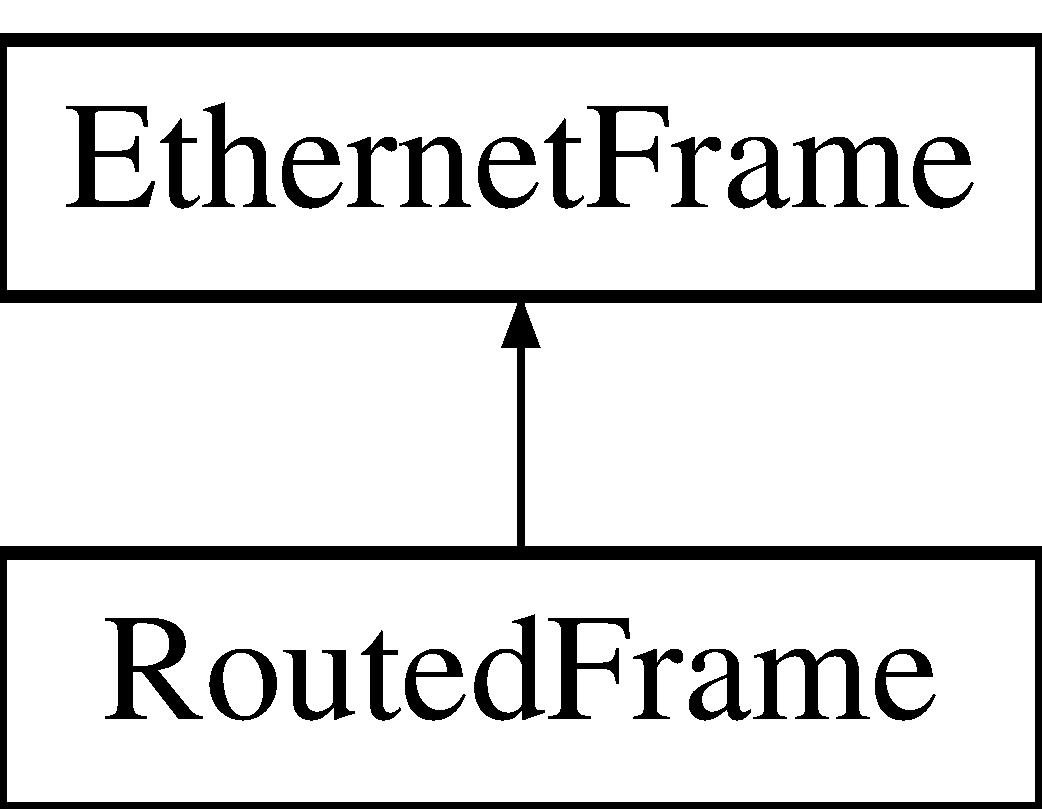
\includegraphics[height=2.000000cm]{classRoutedFrame}
\end{center}
\end{figure}
\subsection*{Public Member Functions}
\begin{DoxyCompactItemize}
\item 
\hypertarget{classRoutedFrame_acce70d6e6faba3c7552a0047310134a7}{{\bfseries Routed\-Frame} (std\-::string topic\-\_\-to\-\_\-publish, std\-::string data, uint8\-\_\-t payload\-\_\-type\-\_\-field, uint32\-\_\-t pack\-\_\-id, uint32\-\_\-t pack\-\_\-sequence\-\_\-num, uint32\-\_\-t frames\-\_\-in\-\_\-pack)}\label{classRoutedFrame_acce70d6e6faba3c7552a0047310134a7}

\item 
\hypertarget{classRoutedFrame_ab19fd22358ff2285bdb1ed30b6f82046}{{\bfseries Routed\-Frame} (unsigned char $\ast$buffer)}\label{classRoutedFrame_ab19fd22358ff2285bdb1ed30b6f82046}

\item 
\hypertarget{classRoutedFrame_a28ff8e7e3ef99fe147cacaa6344ec022}{unsigned long {\bfseries get\-Size} ()}\label{classRoutedFrame_a28ff8e7e3ef99fe147cacaa6344ec022}

\item 
\hypertarget{classRoutedFrame_aac21d89fb44e75b0b875919ae45a24af}{\hyperlink{structstc__frame}{stc\-\_\-frame} {\bfseries get\-Frame\-Struct} ()}\label{classRoutedFrame_aac21d89fb44e75b0b875919ae45a24af}

\item 
\hypertarget{classRoutedFrame_a2d6d1b1017c34be2064151646bd07ce8}{std\-::string {\bfseries get\-Frame\-As\-Network\-String} (\hyperlink{structrouting__entry}{routing\-\_\-entry} rou, unsigned char source\mbox{[}6\mbox{]})}\label{classRoutedFrame_a2d6d1b1017c34be2064151646bd07ce8}

\item 
\hypertarget{classRoutedFrame_a37a8fa4df09a1d3768278b10d0734a5a}{std\-::string {\bfseries get\-Frame\-As\-Network\-String} (uint32\-\_\-t route\-\_\-id, unsigned char next\-\_\-hop\mbox{[}6\mbox{]}, string source\-\_\-host, unsigned char source\mbox{[}6\mbox{]})}\label{classRoutedFrame_a37a8fa4df09a1d3768278b10d0734a5a}

\end{DoxyCompactItemize}
\subsection*{Data Fields}
\begin{DoxyCompactItemize}
\item 
\hypertarget{classRoutedFrame_a95ca682910f52356b264f9ff7ac542db}{struct \hyperlink{structrf__header}{rf\-\_\-header} {\bfseries header\-\_\-}}\label{classRoutedFrame_a95ca682910f52356b264f9ff7ac542db}

\item 
\hypertarget{classRoutedFrame_a8554376bea5ec4b29717348344d4df1a}{std\-::string {\bfseries hostname\-\_\-source\-\_\-}}\label{classRoutedFrame_a8554376bea5ec4b29717348344d4df1a}

\item 
\hypertarget{classRoutedFrame_af73e229c3b7e475d0effb1270a6d9ef9}{std\-::string {\bfseries mc\-\_\-g\-\_\-name\-\_\-}}\label{classRoutedFrame_af73e229c3b7e475d0effb1270a6d9ef9}

\item 
\hypertarget{classRoutedFrame_a126d112f3df60e22a1ad9a61b76eb0e5}{std\-::string {\bfseries topic\-\_\-}}\label{classRoutedFrame_a126d112f3df60e22a1ad9a61b76eb0e5}

\item 
\hypertarget{classRoutedFrame_a929f9207203948d08292aefa95fa09f9}{std\-::string {\bfseries payload\-\_\-}}\label{classRoutedFrame_a929f9207203948d08292aefa95fa09f9}

\item 
\hypertarget{classRoutedFrame_a68abd0cc5671fde03b6bb9b9113fbd95}{bool {\bfseries cr\-\_\-flag}}\label{classRoutedFrame_a68abd0cc5671fde03b6bb9b9113fbd95}

\item 
\hypertarget{classRoutedFrame_abfcf2b1dbebfaf3d6078b9dde576aa59}{bool {\bfseries mc\-\_\-flag}}\label{classRoutedFrame_abfcf2b1dbebfaf3d6078b9dde576aa59}

\item 
\hypertarget{classRoutedFrame_aee77780fb428b97d4c7f99ae901ad635}{bool {\bfseries negative\-\_\-ack\-\_\-type}}\label{classRoutedFrame_aee77780fb428b97d4c7f99ae901ad635}

\item 
\hypertarget{classRoutedFrame_a18469d151e4f4f84a17dfa723cc98f8f}{bool {\bfseries resend\-\_\-flag}}\label{classRoutedFrame_a18469d151e4f4f84a17dfa723cc98f8f}

\item 
\hypertarget{classRoutedFrame_a0ef7137e83b66d78ca77dfb96db47023}{uint16\-\_\-t {\bfseries buffer\-\_\-str\-\_\-len\-\_\-}}\label{classRoutedFrame_a0ef7137e83b66d78ca77dfb96db47023}

\end{DoxyCompactItemize}
\subsection*{Static Public Attributes}
\begin{DoxyCompactItemize}
\item 
\hypertarget{classRoutedFrame_ae502201806de8392281f4d7f216efb6f}{static uint32\-\_\-t {\bfseries frame\-\_\-count\-\_\-stat} = 0}\label{classRoutedFrame_ae502201806de8392281f4d7f216efb6f}

\item 
\hypertarget{classRoutedFrame_ae3db0ff9b4f6fdbe4ca404527f92b5f7}{static uint32\-\_\-t {\bfseries H\-E\-A\-D\-E\-R\-\_\-\-F\-I\-X\-E\-D\-\_\-\-L\-E\-N} = sizeof(\hyperlink{structeh__header}{eh\-\_\-header}) + sizeof(\hyperlink{structrf__header}{rf\-\_\-header})}\label{classRoutedFrame_ae3db0ff9b4f6fdbe4ca404527f92b5f7}

\item 
\hypertarget{classRoutedFrame_a2c12e04a49a8565ac0777c9d185cd876}{static bool {\bfseries enable\-\_\-cooperative\-\_\-relaying} = false}\label{classRoutedFrame_a2c12e04a49a8565ac0777c9d185cd876}

\end{DoxyCompactItemize}


\subsection{Detailed Description}
The class of a routed frame. 

The class contains all needed frame fields and the functions to serialize a frame or desizalied it from a buffer

H\-E\-A\-D\-E\-R O\-F A R\-O\-U\-T\-E\-D F\-R\-A\-M\-E\-: H\-E\-A\-D\-E\-R F\-I\-E\-L\-D\-S\-:
\begin{DoxyItemize}
\item D\-E\-S\-T\-I\-N\-A\-T\-I\-O\-N M\-A\-C
\begin{DoxyItemize}
\item S\-I\-Z\-E\-: 6 Byte
\end{DoxyItemize}
\item S\-O\-U\-R\-C\-E M\-A\-C
\begin{DoxyItemize}
\item S\-I\-Z\-E\-: 6 Byte
\end{DoxyItemize}
\item E\-T\-H\-\_\-\-T\-Y\-P\-E\-\_\-\-F\-I\-E\-L\-D
\begin{DoxyItemize}
\item S\-I\-Z\-E\-: 2 Byte
\end{DoxyItemize}
\item F\-R\-A\-M\-E\-\_\-\-T\-Y\-P\-E
\begin{DoxyItemize}
\item S\-I\-Z\-E\-: 1 Byte
\end{DoxyItemize}
\item D\-E\-S\-T\-I\-N\-A\-T\-I\-O\-N
\begin{DoxyItemize}
\item S\-I\-Z\-E\-: 6 Byte
\end{DoxyItemize}
\item F\-R\-A\-M\-E I\-D
\begin{DoxyItemize}
\item S\-I\-Z\-E\-: 4 Byte
\end{DoxyItemize}
\item R\-O\-U\-T\-E I\-D
\begin{DoxyItemize}
\item S\-I\-Z\-E\-: 4 Byte
\end{DoxyItemize}
\item P\-A\-C\-K\-E\-T I\-D
\begin{DoxyItemize}
\item S\-I\-Z\-E\-: 4 Byte
\end{DoxyItemize}
\item S\-E\-Q\-U\-E\-N\-C\-E N\-U\-M\-B\-E\-R
\begin{DoxyItemize}
\item S\-I\-Z\-E\-: 4 Byte
\end{DoxyItemize}
\item P\-A\-C\-K\-E\-T S\-I\-Z\-E
\begin{DoxyItemize}
\item S\-I\-Z\-E\-: 4 Byte
\end{DoxyItemize}
\item S\-O\-U\-R\-C\-E H\-O\-S\-T Length
\begin{DoxyItemize}
\item S\-I\-Z\-E\-: 4 Byte
\end{DoxyItemize}
\item S\-O\-U\-R\-C\-E H\-O\-S\-T
\begin{DoxyItemize}
\item S\-I\-Z\-E\-: V\-A\-R\-I\-A\-B\-L\-E
\end{DoxyItemize}
\item M\-C G\-R\-O\-U\-P L\-E\-N\-G\-T\-H
\begin{DoxyItemize}
\item S\-I\-Z\-E\-: 4 Byte
\end{DoxyItemize}
\item M\-C G\-R\-O\-U\-P N\-A\-M\-E
\begin{DoxyItemize}
\item S\-I\-Z\-E\-: V\-A\-R\-I\-A\-B\-L\-E
\end{DoxyItemize}
\item T\-O\-P\-I\-C\-\_\-\-L\-E\-N\-G\-T\-H
\begin{DoxyItemize}
\item S\-I\-Z\-E\-: 4 Byte
\end{DoxyItemize}
\item T\-O\-P\-I\-C
\begin{DoxyItemize}
\item S\-I\-Z\-E\-: V\-A\-R\-I\-A\-B\-L\-E
\end{DoxyItemize}
\item P\-A\-Y\-L\-O\-A\-D T\-Y\-P\-E
\begin{DoxyItemize}
\item S\-I\-Z\-E\-: 1 Byte
\end{DoxyItemize}
\item P\-A\-Y\-L\-O\-A\-D\-\_\-\-L\-E\-N\-G\-T\-H
\begin{DoxyItemize}
\item S\-I\-Z\-E\-: 4 Byte
\end{DoxyItemize}
\item P\-A\-Y\-L\-O\-A\-D
\begin{DoxyItemize}
\item S\-I\-Z\-E\-: V\-A\-R\-I\-A\-B\-L\-E
\end{DoxyItemize}
\item F\-L\-A\-G F\-I\-E\-L\-D
\begin{DoxyItemize}
\item S\-I\-Z\-E\-: 1 Byte
\end{DoxyItemize}
\item C\-R\-C32 C\-H\-E\-C\-K\-S\-U\-M
\begin{DoxyItemize}
\item S\-I\-Z\-E\-: 4 Byte 
\end{DoxyItemize}
\end{DoxyItemize}

The documentation for this class was generated from the following files\-:\begin{DoxyCompactItemize}
\item 
src/Routed\-Frame.\-h\item 
src/\hyperlink{RoutedFrame_8cpp}{Routed\-Frame.\-cpp}\end{DoxyCompactItemize}

\hypertarget{classRouteRequest}{\section{Route\-Request Class Reference}
\label{classRouteRequest}\index{Route\-Request@{Route\-Request}}
}
Inheritance diagram for Route\-Request\-:\begin{figure}[H]
\begin{center}
\leavevmode
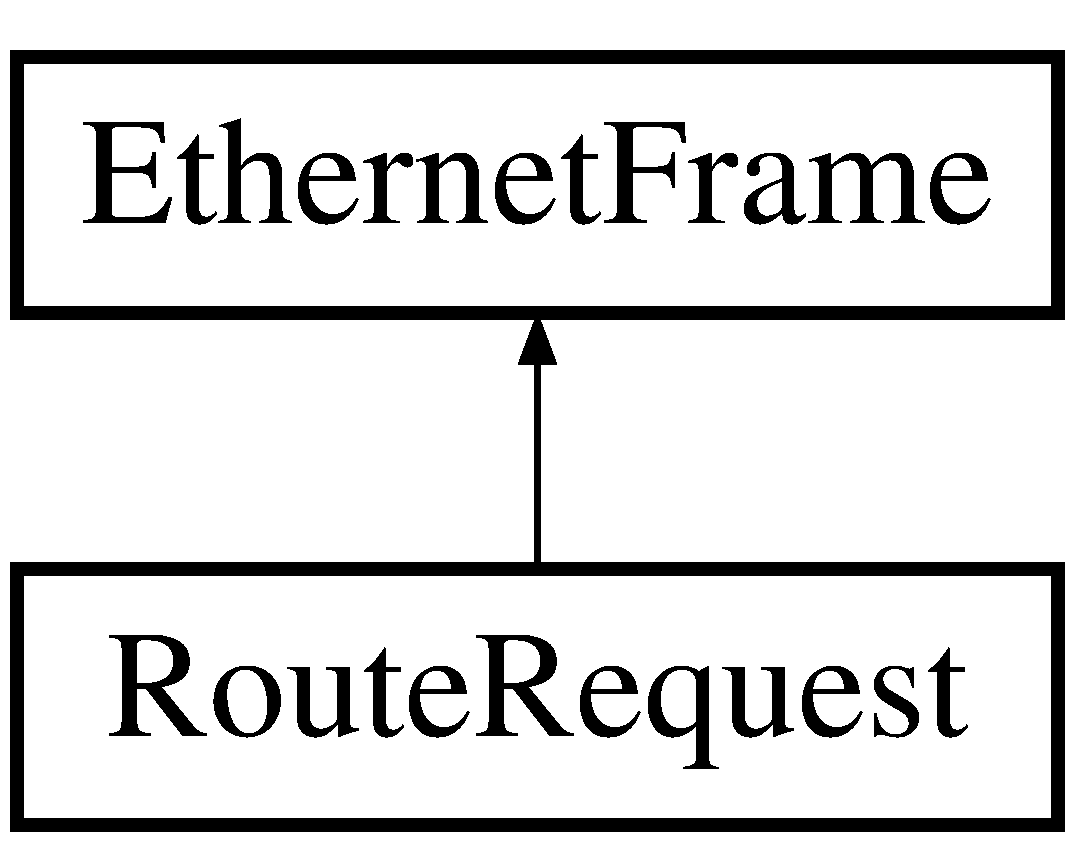
\includegraphics[height=2.000000cm]{classRouteRequest}
\end{center}
\end{figure}
\subsection*{Public Member Functions}
\begin{DoxyCompactItemize}
\item 
\hypertarget{classRouteRequest_a69e3830a1c98ff890d1b0363410ef324}{{\bfseries Route\-Request} (std\-::string my\-\_\-hostname, std\-::string destination, uint16\-\_\-t max\-\_\-hops, bool is\-\_\-multicast)}\label{classRouteRequest_a69e3830a1c98ff890d1b0363410ef324}

\item 
\hypertarget{classRouteRequest_a523ea5e1698dfa54e63ec833054b3bf5}{{\bfseries Route\-Request} (\hyperlink{structroute__request}{route\-\_\-request} req)}\label{classRouteRequest_a523ea5e1698dfa54e63ec833054b3bf5}

\item 
\hypertarget{classRouteRequest_a6841472de2ea7b9059dc95ddda875ec5}{{\bfseries Route\-Request} (unsigned char $\ast$buffer)}\label{classRouteRequest_a6841472de2ea7b9059dc95ddda875ec5}

\item 
\hypertarget{classRouteRequest_a524f45788b485bfaf71b4fd6547d8843}{std\-::string {\bfseries get\-Request\-As\-Network\-String} (unsigned char source\-\_\-mac\mbox{[}6\mbox{]})}\label{classRouteRequest_a524f45788b485bfaf71b4fd6547d8843}

\item 
\hypertarget{classRouteRequest_abf39fb926d81d1070db943578f704c2b}{bool {\bfseries is\-Mac\-In\-Path} (unsigned char \hyperlink{structmac}{mac}\mbox{[}$\,$\mbox{]})}\label{classRouteRequest_abf39fb926d81d1070db943578f704c2b}

\end{DoxyCompactItemize}
\subsection*{Data Fields}
\begin{DoxyCompactItemize}
\item 
\hypertarget{classRouteRequest_a5325f0e37ac4e6098ee927c7a1db944e}{struct \hyperlink{structrreq__header}{rreq\-\_\-header} {\bfseries header\-\_\-}}\label{classRouteRequest_a5325f0e37ac4e6098ee927c7a1db944e}

\item 
\hypertarget{classRouteRequest_a3c7155a0b285f8d2d39b77f76ec3994b}{std\-::string {\bfseries hostname\-\_\-destination\-\_\-}}\label{classRouteRequest_a3c7155a0b285f8d2d39b77f76ec3994b}

\item 
\hypertarget{classRouteRequest_aadb0eeab91313d8bef7b79c847536a03}{std\-::string {\bfseries hostname\-\_\-source\-\_\-}}\label{classRouteRequest_aadb0eeab91313d8bef7b79c847536a03}

\item 
\hypertarget{classRouteRequest_a341660de5ede7819f90ddbeb846a8cd0}{std\-::list$<$ \hyperlink{structmac}{mac} $>$ {\bfseries path\-\_\-l\-\_\-}}\label{classRouteRequest_a341660de5ede7819f90ddbeb846a8cd0}

\item 
\hypertarget{classRouteRequest_a767c5db1ea47707a51ddd74ffed3a6d5}{uint16\-\_\-t {\bfseries buffer\-\_\-str\-\_\-len\-\_\-}}\label{classRouteRequest_a767c5db1ea47707a51ddd74ffed3a6d5}

\item 
\hypertarget{classRouteRequest_ad62235536e529c13904144dc7f9316d2}{bool {\bfseries correct\-\_\-crc\-\_\-}}\label{classRouteRequest_ad62235536e529c13904144dc7f9316d2}

\item 
\hypertarget{classRouteRequest_a76b50927e13bde35727f9bc1ecdd43d6}{bool {\bfseries mc\-\_\-flag\-\_\-}}\label{classRouteRequest_a76b50927e13bde35727f9bc1ecdd43d6}

\end{DoxyCompactItemize}
\subsection*{Static Public Attributes}
\begin{DoxyCompactItemize}
\item 
\hypertarget{classRouteRequest_a7bde218383ec21dac94325fb38ccfc63}{static uint32\-\_\-t {\bfseries req\-\_\-count\-\_\-stat} = 0}\label{classRouteRequest_a7bde218383ec21dac94325fb38ccfc63}

\item 
\hypertarget{classRouteRequest_a974eb2a919005fb4e76ebd0697f77740}{static uint32\-\_\-t {\bfseries H\-E\-A\-D\-E\-R\-\_\-\-F\-I\-X\-E\-D\-\_\-\-L\-E\-N} = sizeof(\hyperlink{structeh__header}{eh\-\_\-header}) + sizeof(\hyperlink{structrreq__header}{rreq\-\_\-header})}\label{classRouteRequest_a974eb2a919005fb4e76ebd0697f77740}

\end{DoxyCompactItemize}


The documentation for this class was generated from the following files\-:\begin{DoxyCompactItemize}
\item 
src/Route\-Request.\-h\item 
src/Route\-Request.\-cpp\end{DoxyCompactItemize}

\hypertarget{classRouteResponse}{\section{Route\-Response Class Reference}
\label{classRouteResponse}\index{Route\-Response@{Route\-Response}}
}
\subsection*{Public Member Functions}
\begin{DoxyCompactItemize}
\item 
\hypertarget{classRouteResponse_a897437599b52149a64d005407b778fdd}{{\bfseries Route\-Response} (\hyperlink{classRouteRequest}{Route\-Request} req, unsigned char \hyperlink{structmac}{mac}\mbox{[}6\mbox{]}, uint8\-\_\-t root\-\_\-distance)}\label{classRouteResponse_a897437599b52149a64d005407b778fdd}

\item 
\hypertarget{classRouteResponse_a47e56d193254e70eccd7be64d80180c6}{{\bfseries Route\-Response} (unsigned char $\ast$buffer)}\label{classRouteResponse_a47e56d193254e70eccd7be64d80180c6}

\item 
\hypertarget{classRouteResponse_a69a843212ab6c0dfc1fa6354e124399b}{int {\bfseries Get\-Crc32} (const std\-::string \&my\-\_\-string)}\label{classRouteResponse_a69a843212ab6c0dfc1fa6354e124399b}

\item 
\hypertarget{classRouteResponse_ab45b7284ad65c5c88613b048af038f12}{std\-::string {\bfseries get\-Response\-As\-Network\-String} (unsigned char source\-\_\-mac\mbox{[}6\mbox{]})}\label{classRouteResponse_ab45b7284ad65c5c88613b048af038f12}

\end{DoxyCompactItemize}
\subsection*{Data Fields}
\begin{DoxyCompactItemize}
\item 
\hypertarget{classRouteResponse_a094f4f46526b2efca6cba02d02d2b5a1}{struct ethhdr {\bfseries eh\-\_\-}}\label{classRouteResponse_a094f4f46526b2efca6cba02d02d2b5a1}

\item 
\hypertarget{classRouteResponse_a9c4ac4d3e69ade05d76debd85b31f9aa}{unsigned char {\bfseries mac\-\_\-current\-\_\-hop\-\_\-} \mbox{[}6\mbox{]}}\label{classRouteResponse_a9c4ac4d3e69ade05d76debd85b31f9aa}

\item 
\hypertarget{classRouteResponse_af4b40eb0ae85e1c7bf6c92adac9183fd}{unsigned char {\bfseries mac\-\_\-next\-\_\-hop\-\_\-} \mbox{[}6\mbox{]}}\label{classRouteResponse_af4b40eb0ae85e1c7bf6c92adac9183fd}

\item 
\hypertarget{classRouteResponse_a43362637d4898bd5e9b907970243e85a}{unsigned char {\bfseries mac\-\_\-previous\-\_\-hop\-\_\-} \mbox{[}6\mbox{]}}\label{classRouteResponse_a43362637d4898bd5e9b907970243e85a}

\item 
\hypertarget{classRouteResponse_aee9346caf4415e846614655426e7dcd0}{uint32\-\_\-t {\bfseries request\-\_\-id\-\_\-}}\label{classRouteResponse_aee9346caf4415e846614655426e7dcd0}

\item 
\hypertarget{classRouteResponse_a0bb239b2ce9e40b4b0187e379d7fa732}{std\-::string {\bfseries hostname\-\_\-source\-\_\-}}\label{classRouteResponse_a0bb239b2ce9e40b4b0187e379d7fa732}

\item 
\hypertarget{classRouteResponse_ada7f69348aaa0f1eadb5f2b84a06b812}{uint32\-\_\-t {\bfseries hop\-\_\-count\-\_\-}}\label{classRouteResponse_ada7f69348aaa0f1eadb5f2b84a06b812}

\item 
\hypertarget{classRouteResponse_a3b0c2b5dffbbbd2a1a6364e68d5ea318}{uint32\-\_\-t {\bfseries current\-\_\-hop\-\_\-}}\label{classRouteResponse_a3b0c2b5dffbbbd2a1a6364e68d5ea318}

\item 
\hypertarget{classRouteResponse_a65445b7f0ce2cdcc77c4aa3cc985a4d7}{std\-::list$<$ \hyperlink{structmac}{mac} $>$ {\bfseries path\-\_\-l\-\_\-}}\label{classRouteResponse_a65445b7f0ce2cdcc77c4aa3cc985a4d7}

\item 
\hypertarget{classRouteResponse_a85021e9523087b3ba0c6f9777393dd8b}{bool {\bfseries correct\-\_\-crc\-\_\-}}\label{classRouteResponse_a85021e9523087b3ba0c6f9777393dd8b}

\item 
\hypertarget{classRouteResponse_a4cdc1ebbb5a8e1e733a8b9434ce10be8}{uint8\-\_\-t {\bfseries mc\-\_\-flag\-\_\-}}\label{classRouteResponse_a4cdc1ebbb5a8e1e733a8b9434ce10be8}

\item 
\hypertarget{classRouteResponse_a4f2c9629843e8ec7cbdc5c4c8893add3}{uint8\-\_\-t {\bfseries root\-\_\-distance}}\label{classRouteResponse_a4f2c9629843e8ec7cbdc5c4c8893add3}

\end{DoxyCompactItemize}
\subsection*{Static Public Attributes}
\begin{DoxyCompactItemize}
\item 
\hypertarget{classRouteResponse_aa16bbeb6d1013a671756a131c9d8dd7a}{static uint32\-\_\-t {\bfseries H\-E\-A\-D\-E\-R\-\_\-\-F\-I\-X\-E\-D\-\_\-\-L\-E\-N} = 37}\label{classRouteResponse_aa16bbeb6d1013a671756a131c9d8dd7a}

\end{DoxyCompactItemize}


The documentation for this class was generated from the following files\-:\begin{DoxyCompactItemize}
\item 
src/Route\-Response.\-h\item 
src/Route\-Response.\-cpp\end{DoxyCompactItemize}

\hypertarget{structrouting__entry}{\section{routing\-\_\-entry Struct Reference}
\label{structrouting__entry}\index{routing\-\_\-entry@{routing\-\_\-entry}}
}
\subsection*{Public Member Functions}
\begin{DoxyCompactItemize}
\item 
\hypertarget{structrouting__entry_a3b336fc641f1e1676c50291e00c91803}{{\bfseries routing\-\_\-entry} (string hname\-\_\-src, uint32\-\_\-t id)}\label{structrouting__entry_a3b336fc641f1e1676c50291e00c91803}

\item 
\hypertarget{structrouting__entry_a761b7e9e6dcfb91df4332b4deda24345}{bool {\bfseries same\-Path} (\hyperlink{structrouting__entry}{routing\-\_\-entry} r)}\label{structrouting__entry_a761b7e9e6dcfb91df4332b4deda24345}

\item 
\hypertarget{structrouting__entry_a769cebc3f8735380c7f3bda9a3de8395}{bool {\bfseries operator==} (const \hyperlink{structrouting__entry}{routing\-\_\-entry} \&st)}\label{structrouting__entry_a769cebc3f8735380c7f3bda9a3de8395}

\end{DoxyCompactItemize}
\subsection*{Data Fields}
\begin{DoxyCompactItemize}
\item 
\hypertarget{structrouting__entry_a241406739cb6984e59f12ab1b523506a}{std\-::string {\bfseries hostname\-\_\-destination}}\label{structrouting__entry_a241406739cb6984e59f12ab1b523506a}

\item 
\hypertarget{structrouting__entry_a131cfb32c1d84f883b79730048597588}{std\-::string {\bfseries hostname\-\_\-source}}\label{structrouting__entry_a131cfb32c1d84f883b79730048597588}

\item 
\hypertarget{structrouting__entry_aa2eeddbcf5fadaacfe71e71b04d69a2c}{std\-::list$<$ \hyperlink{structmac}{mac} $>$ {\bfseries mac\-\_\-path\-\_\-l}}\label{structrouting__entry_aa2eeddbcf5fadaacfe71e71b04d69a2c}

\item 
\hypertarget{structrouting__entry_a87aed279f56da4bb9eb6b84933a9fc77}{uint32\-\_\-t {\bfseries id}}\label{structrouting__entry_a87aed279f56da4bb9eb6b84933a9fc77}

\item 
\hypertarget{structrouting__entry_aa4864549a92479aa74753f1acbbef88d}{unsigned long {\bfseries ts}}\label{structrouting__entry_aa4864549a92479aa74753f1acbbef88d}

\item 
\hypertarget{structrouting__entry_aad5e2cc7e2110927f27d44d9cc41372f}{unsigned char {\bfseries next\-\_\-hop} \mbox{[}6\mbox{]}}\label{structrouting__entry_aad5e2cc7e2110927f27d44d9cc41372f}

\item 
\hypertarget{structrouting__entry_a08d92725236e702d30b11279c1569cc6}{unsigned char {\bfseries previous\-\_\-hop} \mbox{[}6\mbox{]}}\label{structrouting__entry_a08d92725236e702d30b11279c1569cc6}

\item 
\hypertarget{structrouting__entry_a3d36bae4fbf7192dbdd4ced2a4eef634}{uint16\-\_\-t {\bfseries hobs}}\label{structrouting__entry_a3d36bae4fbf7192dbdd4ced2a4eef634}

\item 
\hypertarget{structrouting__entry_aae9850b8704f7a184be5a21335125c99}{uint16\-\_\-t {\bfseries current\-\_\-hop}}\label{structrouting__entry_aae9850b8704f7a184be5a21335125c99}

\item 
\hypertarget{structrouting__entry_a6ad77f5398f8fe97485b72f5f947e319}{uint8\-\_\-t {\bfseries root\-\_\-distance}}\label{structrouting__entry_a6ad77f5398f8fe97485b72f5f947e319}

\item 
\hypertarget{structrouting__entry_a56af04dbe25b1ad2f4f209582911eaec}{bool {\bfseries cr\-\_\-entry}}\label{structrouting__entry_a56af04dbe25b1ad2f4f209582911eaec}

\end{DoxyCompactItemize}


The documentation for this struct was generated from the following file\-:\begin{DoxyCompactItemize}
\item 
src/structs.\-h\end{DoxyCompactItemize}

\hypertarget{structrreq__header}{\section{rreq\-\_\-header Struct Reference}
\label{structrreq__header}\index{rreq\-\_\-header@{rreq\-\_\-header}}
}
\subsection*{Data Fields}
\begin{DoxyCompactItemize}
\item 
\hypertarget{structrreq__header_a463a2c2d5a33a4efc9b9f4fe281c0f54}{uint8\-\_\-t {\bfseries frame\-\_\-type}}\label{structrreq__header_a463a2c2d5a33a4efc9b9f4fe281c0f54}

\item 
\hypertarget{structrreq__header_a715128ca69f8609891a5ba02936ec1e7}{uint32\-\_\-t {\bfseries id}}\label{structrreq__header_a715128ca69f8609891a5ba02936ec1e7}

\item 
\hypertarget{structrreq__header_a0bd7facab67ef6b092415d7e9d541a67}{uint32\-\_\-t {\bfseries hop\-\_\-count}}\label{structrreq__header_a0bd7facab67ef6b092415d7e9d541a67}

\item 
\hypertarget{structrreq__header_ab93ee70a23ce9881a8ce98082c0ca277}{uint32\-\_\-t {\bfseries hop\-\_\-limit}}\label{structrreq__header_ab93ee70a23ce9881a8ce98082c0ca277}

\item 
\hypertarget{structrreq__header_a02a72c2114308d8207377fcdb1e921ea}{uint8\-\_\-t {\bfseries flag\-\_\-field}}\label{structrreq__header_a02a72c2114308d8207377fcdb1e921ea}

\item 
\hypertarget{structrreq__header_a4b483117981c20b91ae391fa46de1b3c}{uint32\-\_\-t {\bfseries hostname\-\_\-source\-\_\-len}}\label{structrreq__header_a4b483117981c20b91ae391fa46de1b3c}

\item 
\hypertarget{structrreq__header_ac359770edf9b683681c83b82e3d5d3bf}{uint32\-\_\-t {\bfseries hostname\-\_\-destination\-\_\-len}}\label{structrreq__header_ac359770edf9b683681c83b82e3d5d3bf}

\end{DoxyCompactItemize}


The documentation for this struct was generated from the following file\-:\begin{DoxyCompactItemize}
\item 
src/Route\-Request.\-h\end{DoxyCompactItemize}

\hypertarget{structstc__ack}{\section{stc\-\_\-ack Struct Reference}
\label{structstc__ack}\index{stc\-\_\-ack@{stc\-\_\-ack}}
}
\subsection*{Public Member Functions}
\begin{DoxyCompactItemize}
\item 
\hypertarget{structstc__ack_a990edbb8d4cf9f9ac729ddc8cf6cb71d}{bool {\bfseries operator==} (const \hyperlink{structstc__ack}{stc\-\_\-ack} \&st)}\label{structstc__ack_a990edbb8d4cf9f9ac729ddc8cf6cb71d}

\end{DoxyCompactItemize}
\subsection*{Data Fields}
\begin{DoxyCompactItemize}
\item 
\hypertarget{structstc__ack_aa3ef3373865a4937672e1e221d72cf9c}{std\-::string {\bfseries network\-\_\-string}}\label{structstc__ack_aa3ef3373865a4937672e1e221d72cf9c}

\item 
\hypertarget{structstc__ack_a14df6fc61b91a0161fd0573bfa6f210d}{uint32\-\_\-t {\bfseries frame\-\_\-id}}\label{structstc__ack_a14df6fc61b91a0161fd0573bfa6f210d}

\item 
\hypertarget{structstc__ack_aaeadf5c169f34b762e5f64dc22872cac}{uint8\-\_\-t {\bfseries retransmitted}}\label{structstc__ack_aaeadf5c169f34b762e5f64dc22872cac}

\item 
\hypertarget{structstc__ack_a42b6c5b7677399ac1d4293ac7fc13b96}{unsigned char {\bfseries mac} \mbox{[}6\mbox{]}}\label{structstc__ack_a42b6c5b7677399ac1d4293ac7fc13b96}

\end{DoxyCompactItemize}


The documentation for this struct was generated from the following file\-:\begin{DoxyCompactItemize}
\item 
src/structs.\-h\end{DoxyCompactItemize}

\hypertarget{structstc__frame}{\section{stc\-\_\-frame Struct Reference}
\label{structstc__frame}\index{stc\-\_\-frame@{stc\-\_\-frame}}
}
\subsection*{Public Member Functions}
\begin{DoxyCompactItemize}
\item 
\hypertarget{structstc__frame_aca7549c3afce65dadb2364be17e057cf}{void {\bfseries print\-\_\-frame} ()}\label{structstc__frame_aca7549c3afce65dadb2364be17e057cf}

\item 
\hypertarget{structstc__frame_a8c9f585c3f8dadaf0c4e3d0d06e84297}{bool {\bfseries operator==} (const \hyperlink{structstc__frame}{stc\-\_\-frame} \&st)}\label{structstc__frame_a8c9f585c3f8dadaf0c4e3d0d06e84297}

\end{DoxyCompactItemize}
\subsection*{Data Fields}
\begin{DoxyCompactItemize}
\item 
\hypertarget{structstc__frame_a3a8da73a7a618941115ab6853de30a01}{std\-::string {\bfseries network\-\_\-string}}\label{structstc__frame_a3a8da73a7a618941115ab6853de30a01}

\item 
\hypertarget{structstc__frame_a5b38e52bcffb8057430e290594b15232}{uint32\-\_\-t {\bfseries frame\-\_\-id}}\label{structstc__frame_a5b38e52bcffb8057430e290594b15232}

\item 
\hypertarget{structstc__frame_a8735d03fa5449af5e31f2111ee4381b5}{uint8\-\_\-t {\bfseries retransmitted}}\label{structstc__frame_a8735d03fa5449af5e31f2111ee4381b5}

\item 
\hypertarget{structstc__frame_a7f3b7f11f950ae16689e72f213d1cc73}{bool {\bfseries cr}}\label{structstc__frame_a7f3b7f11f950ae16689e72f213d1cc73}

\item 
\hypertarget{structstc__frame_a16e5e51a2b2abf7e3ea96e27dde70527}{unsigned char {\bfseries mac} \mbox{[}6\mbox{]}}\label{structstc__frame_a16e5e51a2b2abf7e3ea96e27dde70527}

\item 
\hypertarget{structstc__frame_a6fe26bc08e6b1a94d02b1ad9b07b9714}{uint8\-\_\-t {\bfseries type}}\label{structstc__frame_a6fe26bc08e6b1a94d02b1ad9b07b9714}

\item 
\hypertarget{structstc__frame_a297a8359a1279b4647324cd9db100d4b}{std\-::string {\bfseries hostname\-\_\-source}}\label{structstc__frame_a297a8359a1279b4647324cd9db100d4b}

\item 
\hypertarget{structstc__frame_a91ad7ccd8878306de0b47791000be524}{std\-::string {\bfseries mc\-\_\-group}}\label{structstc__frame_a91ad7ccd8878306de0b47791000be524}

\item 
\hypertarget{structstc__frame_a1ce6c3532b0d8d835a5c5b3f28cec2c7}{unsigned long {\bfseries ts}}\label{structstc__frame_a1ce6c3532b0d8d835a5c5b3f28cec2c7}

\end{DoxyCompactItemize}


The documentation for this struct was generated from the following file\-:\begin{DoxyCompactItemize}
\item 
src/Ethernet\-Frame.\-h\end{DoxyCompactItemize}

\hypertarget{structstc__packet}{\section{stc\-\_\-packet Struct Reference}
\label{structstc__packet}\index{stc\-\_\-packet@{stc\-\_\-packet}}
}
\subsection*{Public Member Functions}
\begin{DoxyCompactItemize}
\item 
\hypertarget{structstc__packet_a797f8f9c8d35e9a99b7afa4185109bee}{{\bfseries stc\-\_\-packet} (string source, string mc\-\_\-g, uint32\-\_\-t p\-\_\-id)}\label{structstc__packet_a797f8f9c8d35e9a99b7afa4185109bee}

\item 
\hypertarget{structstc__packet_a57afe0090b0d85952b3e1b7d2b6aced1}{bool {\bfseries operator==} (const \hyperlink{structstc__packet}{stc\-\_\-packet} \&p)}\label{structstc__packet_a57afe0090b0d85952b3e1b7d2b6aced1}

\end{DoxyCompactItemize}
\subsection*{Data Fields}
\begin{DoxyCompactItemize}
\item 
\hypertarget{structstc__packet_ad9a994b0dae353114552760e5a7e2669}{string {\bfseries src}}\label{structstc__packet_ad9a994b0dae353114552760e5a7e2669}

\item 
\hypertarget{structstc__packet_aa568f4dbc7e2889b4749abfa75c0bd0e}{string {\bfseries mc\-\_\-group}}\label{structstc__packet_aa568f4dbc7e2889b4749abfa75c0bd0e}

\item 
\hypertarget{structstc__packet_aa68a7faca167465473001a68aa673df6}{uint32\-\_\-t {\bfseries id}}\label{structstc__packet_aa68a7faca167465473001a68aa673df6}

\item 
\hypertarget{structstc__packet_a9afbe85ef7a2a91b8332ea1022fec75e}{unsigned long {\bfseries ts}}\label{structstc__packet_a9afbe85ef7a2a91b8332ea1022fec75e}

\end{DoxyCompactItemize}


The documentation for this struct was generated from the following file\-:\begin{DoxyCompactItemize}
\item 
src/structs.\-h\end{DoxyCompactItemize}

\hypertarget{structstc__RoutedFrame}{\section{stc\-\_\-\-Routed\-Frame Struct Reference}
\label{structstc__RoutedFrame}\index{stc\-\_\-\-Routed\-Frame@{stc\-\_\-\-Routed\-Frame}}
}
\subsection*{Public Member Functions}
\begin{DoxyCompactItemize}
\item 
\hypertarget{structstc__RoutedFrame_af57a16889993984ff900d612aa8cd426}{bool {\bfseries operator==} (const \hyperlink{structstc__RoutedFrame}{stc\-\_\-\-Routed\-Frame} \&st)}\label{structstc__RoutedFrame_af57a16889993984ff900d612aa8cd426}

\end{DoxyCompactItemize}
\subsection*{Data Fields}
\begin{DoxyCompactItemize}
\item 
\hypertarget{structstc__RoutedFrame_a7f85a4397b4d537344e2305553320234}{\hyperlink{classRoutedFrame}{Routed\-Frame} {\bfseries frame}}\label{structstc__RoutedFrame_a7f85a4397b4d537344e2305553320234}

\item 
\hypertarget{structstc__RoutedFrame_a09259ebbd351886987d3265bbb067ac8}{uint8\-\_\-t {\bfseries retransmitted}}\label{structstc__RoutedFrame_a09259ebbd351886987d3265bbb067ac8}

\item 
\hypertarget{structstc__RoutedFrame_a5cdfc743edd1d9d07cdb438bc5d16448}{bool {\bfseries frame\-\_\-is\-\_\-ack}}\label{structstc__RoutedFrame_a5cdfc743edd1d9d07cdb438bc5d16448}

\item 
\hypertarget{structstc__RoutedFrame_a74ab7f94fa4d89a4d57f1cc0daa6c677}{string {\bfseries hostname\-\_\-destination}}\label{structstc__RoutedFrame_a74ab7f94fa4d89a4d57f1cc0daa6c677}

\item 
\hypertarget{structstc__RoutedFrame_ac983ef308aa19abcc8bb34aa67026a2c}{unsigned char {\bfseries mac} \mbox{[}6\mbox{]}}\label{structstc__RoutedFrame_ac983ef308aa19abcc8bb34aa67026a2c}

\item 
\hypertarget{structstc__RoutedFrame_a371a0406c0644354132e9303463ba0bc}{unsigned long {\bfseries time\-\_\-stamp}}\label{structstc__RoutedFrame_a371a0406c0644354132e9303463ba0bc}

\end{DoxyCompactItemize}


The documentation for this struct was generated from the following file\-:\begin{DoxyCompactItemize}
\item 
src/structs.\-h\end{DoxyCompactItemize}

\chapter{File Documentation}
\hypertarget{Packet_8h}{\section{src/\-Packet.h File Reference}
\label{Packet_8h}\index{src/\-Packet.\-h@{src/\-Packet.\-h}}
}


Network layer packet definition.  


\subsection*{Data Structures}
\begin{DoxyCompactItemize}
\item 
class \hyperlink{classPacket}{Packet}
\begin{DoxyCompactList}\small\item\em The packet class for network layer packets. \end{DoxyCompactList}\end{DoxyCompactItemize}


\subsection{Detailed Description}
Network layer packet definition. \begin{DoxyDate}{Date}
21.\-08.\-2013 
\end{DoxyDate}
\begin{DoxyAuthor}{Author}
Günther Cwioro, Torsten Andre 
\end{DoxyAuthor}

\hypertarget{PositionSubscriber_8h}{\section{src/\-Position\-Subscriber.h File Reference}
\label{PositionSubscriber_8h}\index{src/\-Position\-Subscriber.\-h@{src/\-Position\-Subscriber.\-h}}
}
\subsection*{Data Structures}
\begin{DoxyCompactItemize}
\item 
class \hyperlink{classPositionSubscriber}{Position\-Subscriber}
\begin{DoxyCompactList}\small\item\em Subscripes to the position of the stage simulation. \end{DoxyCompactList}\end{DoxyCompactItemize}


\subsection{Detailed Description}
\begin{DoxyDate}{Date}
11.\-11.\-2013 
\end{DoxyDate}
\begin{DoxyAuthor}{Author}
\-: Günther Cwioro, Torsten Andre 
\end{DoxyAuthor}

\hypertarget{RoutedFrame_8cpp}{\section{src/\-Routed\-Frame.cpp File Reference}
\label{RoutedFrame_8cpp}\index{src/\-Routed\-Frame.\-cpp@{src/\-Routed\-Frame.\-cpp}}
}


Network layer packet definition.  


{\ttfamily \#include $<$string$>$}\\*
{\ttfamily \#include \char`\"{}Routed\-Frame.\-h\char`\"{}}\\*
{\ttfamily \#include \char`\"{}Ethernet\-Frame.\-h\char`\"{}}\\*


\subsection{Detailed Description}
Network layer packet definition. \begin{DoxyDate}{Date}
29.\-07.\-2013 
\end{DoxyDate}
\begin{DoxyAuthor}{Author}
Günther Cwioro, Torsten Andre 
\end{DoxyAuthor}

%--- End generated contents ---

% Index
\newpage
\phantomsection
\addcontentsline{toc}{chapter}{Index}
\printindex

\end{document}
